\documentclass [11pt]{article}
%Two colums
%\documentclass[twocolumn]{article}
% \usepackage[colorlinks,bookmarksopen,bookmarksnumbered,citecolor=blue,urlcolor=blue]{hyperref}
% \newcommand\BibTeX{{\rmfamily B\kern-.05em \textsc{i\kern-.025em b}\kern-.08emT\kern-.1667em\lower.7ex\hbox{E}\kern-.125emX}}
\usepackage{amsmath}
\usepackage[top=25.4truemm,bottom=25.4truemm,left=25.4truemm,right=25.4truemm]{geometry}
\usepackage{mathrsfs}
\usepackage{amsfonts}
\usepackage[table]{xcolor} % For color
\usepackage{graphicx}
\usepackage{caption}   
\usepackage{subcaption}          
\usepackage{breqn}                      
\usepackage{booktabs}    
\usepackage{tabularx}
\usepackage{array} % Add this in your preamble
\usepackage{float} % For table placement
\usepackage[toc,page]{appendix}     
\usepackage{enumitem}  
\usepackage{lscape} 
%\usepackage{ascmac}     
\usepackage{rotating}   
% \usepackage[natbibapa]{apacite}    
\usepackage{url}
\usepackage{setspace}  
\usepackage{adjustbox} 
\usepackage{pdfpages}
\usepackage{hyperref} 
\usepackage{tikz}
\usepackage{pdflscape}
\usepackage{amsmath, amssymb, amsthm, mathtools}

%============================
% Theorems
%============================

\theoremstyle{plain}
\newtheorem{theorem}{Theorem}[section]
\newtheorem{proposition}[theorem]{Proposition}
\newtheorem{lemma}[theorem]{Lema}
\newtheorem{corollary}[theorem]{Corollary}

\theoremstyle{definition}
\newtheorem{definition}[theorem]{Definition}
\newtheorem{example}[theorem]{Examples}
\newtheorem{exercise}[theorem]{Exercises}

\theoremstyle{remark}
\newtheorem{remark}[theorem]{Remark}

%============================
% Operators & macros
%============================

\DeclareMathOperator{\spec}{spec}
\DeclareMathOperator{\diag}{diag}
\newcommand{\R}{\mathbb{R}}
\newcommand{\N}{\mathbb{N}}
\newcommand{\1}{\bm{1}}
\newcommand{\Prob}{\mathbb{P}}
\newcommand{\E}{\mathbb{E}}
\newcommand{\ip}[2]{\left\langle #1,#2\right\rangle}
\newcommand{\sym}[1]{\ifmmode^{#1}\else\(^{#1}\)\fi}

\hypersetup{colorlinks=true, citecolor=blue, urlcolor  = blue, linkcolor = black} 

\usepackage[natbibapa]{apacite}
\AtBeginDocument{%
   \renewcommand{\BRetrievedFrom}{}  % <=== This addresses your main request (no "Retrieved from")
}
 
\graphicspath{{Figure}}
 
\begin{document}

\title{Water Treatment, E. coli in Drinking Water, and Diarrhea:\\
Causal Inference Using Double/Debiased Machine Learning%\footnote{I am grateful to ...Any errors are my own.}
}

\author{Juan Alvaro Diaz Raimond Kedilhac\footnote{Universidad Panamericana, School of Government and Economics, Augusto Rodin No. 498, Col. Insurgentes Mixcoac, Benito Juárez, Ciudad de México 03920, E-mail: 0251520@up.edu.mx}\\
\textit{Universidad Panamericana}\\
~\\
Akito Kamei\footnote{Universidad Panamericana, School of Government and Economics, Augusto Rodin No. 498, Col. Insurgentes Mixcoac, Benito Juárez, Ciudad de México 03920, E-mail: akamei@up.edu.mx}\\
\textit{Universidad Panamericana}\\
}
\date{\today}
\maketitle  

%%Key numbers used in the paper
\newcommand{\ToTSample}{59,633}
\newcommand{\ToTSelected}{64,420}

%%%%%%%%%%%%%%%%%%%%%%%%%%%%%%%%%%%%%%%%%%%%
\begin{center}
\textbf{Abstract}
\end{center}  
\begin{singlespace}
Household decisions to treat drinking water are endogenous to a wide range of socioeconomic, environmental, and behavioral factors, making causal inference challenging in observational settings. This paper estimates the causal effects of household water treatment on E. coli contamination and child diarrhea using Double/Debiased Machine Learning (DDML), a framework designed to address high-dimensional confounding. The analysis draws on MICS data from \ToTSample{} households across 25 countries in Sub-Saharan Africa, Latin America, and Asia and incorporates objective measures of water quality based on E. coli testing. The DDML estimates indicate that conventional OLS models slightly overstate the effectiveness of household water treatment in reducing E. coli contamination, while still confirming a statistically significant causal effect. Among treatment methods, boiling produces the largest reductions in E. coli contamination, whereas chlorination also yields statistically significant but smaller effects. The DDML estimates further suggest that household water treatment reduces the incidence of child diarrhea. However, predictive performance for diarrhea remains limited, with substantial residual variation reflecting the inherently complex and difficult-to-predict nature of diarrheal disease transmission. Overall, the findings provide robust cross-country evidence that household water treatment improves drinking water quality.
\\(187 words)
\end{singlespace}

\doublespacing 

\noindent
\textbf{Funding:}
No funding was received for this research.

\noindent 
JEL Classification: I12, I15 \\
% I12 – Health Behavior
% I15	Health and Economic Development
% Q54: Weather; Natural Disasters and their Management; Global Warming
\noindent
Keywords: Water Treatment, Water Quality, WASH, E. coli; Child diarrhea, Causal Inference

\iffalse
\begin{itemize}
\item \href{https://docs.google.com/document/d/1VpyidSOLfcp7vShdWENKIl0B17a6ory5JjOUVZ8X8vY/edit?tab=t.0}{Google Docs}
\item \href{https://www.dropbox.com/scl/fo/vn55vxpshgnggq5omz1fe/AFpfqHtUH1Q1MqyJ8SoMAQ8?rlkey=h3qh2m9d6pxrxe7q7e071ljeo&dl=0}{Dropbox}
\item \href{https://docs.doubleml.org/stable/guide/guide.html}{Double ML}
\end{itemize}
\fi

\clearpage

\section*{Journal}
\begin{itemize}
	\item High: The Lancet Global Health
	\item High: Journal of Human Resources\\
	Bennett, D. (2008). Does clean water make you dirty? Water supply and sanitation in the rural Philippines.
	\item Journal of Health Economics (High and not good match?)
	\item Mid-high: Economic Development and Cultural Change
	\item Mid-high: \textbf{World Development}
	\item Mid-high: World Bank Research Observer\\
	\url{https://academic.oup.com/wbro/article-abstract/22/1/1/1655339}
	\item Mid-high: World Bank Economic Review
	\item Mid-high: Oxford
	\item World Development Perspectives
	\item Oxford Development Studies
	\item	BMC Public Health
	\item Environmental Health Perspectives – 10.1 (Robert Bain)
	\item BMC Public Health
	\item BMJ\\
Clasen, T., Schmidt, W.-P., Rabie, T., Roberts, I., \& Cairncross, S. (2007). Interventions to improve water quality for preventing diarrhoea: systematic review and meta-analysis. BMJ, 334(7597), 782. https://doi.org/10.1136/bmj.39118.489931.BE.
\end{itemize}

\iffalse
\clearpage
\section*{LANCET Specific}  
\subsection{Research in context}  
Evidence before this study This section should include a description of all the evidence that the authors considered before undertaking this study. Authors should briefly state: the sources (databases, journal or
book reference lists, etc) searched; the criteria used to include or exclude studies (including the exact start and end dates of the search), which should not be limited to English language publications; the search terms used; the quality (risk of bias) of that evidence; and the pooled estimate derived from meta-analysis of the evidence, if appropriate.

\subsection{Added value of this study}  
Authors should describe here how their findings add value to the existing evidence.

\subsection{Implications of all the available evidence}  
Authors should state the implications for practice or policy and future research of their study combined with existing evidence. Research in context panels should not contain references; key studies mentioned here should be referenced in the main text.
\fi

\clearpage
\section{Introduction} 
Despite substantial progress in global health, an estimated 4.4 billion people across 135 low- and middle-income countries still lack access to safe drinking water \cite{greenwood2024mapping}. Enteric infectious diseases continue to pose a major public health challenge, claiming more than 1 million lives worldwide in 2023 and remaining among the ten leading causes of death among children under five \citep{GBD2023Diarrhoeal2026}.

Although laboratory studies demonstrate that household water treatment can effectively reduce E. coli contamination under controlled conditions \citep{rice1999chlorine}, its effectiveness under naturally occurring household behavior remains uncertain. Because households endogenously choose whether to treat their water, which treatment method to adopt, and how consistently to apply it, estimating the causal effects of household water treatment using observational data is challenging. As a result, while experimental evidence is abundant \citep{arnold2007treating,pickering2019wash,luby2018effects}, credible evidence on the causal effects of household water treatment in non-experimental settings remains limited.

Using MICS data from a non-experimental setting, this paper estimates the causal impact of household water treatment on E. coli contamination and child diarrhea using Double/Debiased Machine Learning (DDML), a framework designed for settings with high-dimensional confounding. The analysis draws on 59,633 households across 25 countries in Sub-Saharan Africa, Latin America, and Asia and incorporates objective measures of water quality. By combining flexible machine-learning methods with robust causal inference techniques, the study addresses key identification challenges common in observational WASH data.

The results suggest that standard OLS specifications modestly exaggerate the impact of household water treatment on E. coli contamination. After accounting for high-dimensional confounding using Double/Debiased Machine Learning (DDML), the estimated effects become smaller but remain statistically significant. Boiling emerges as the most effective treatment method for reducing E. coli, while chlorination also yields statistically significant, though smaller, reductions. The DDML estimates further suggest that household water treatment lowers the likelihood of childhood diarrhea, but predictive performance for diarrhea remains limited, highlighting the substantial residual variation and the multifactorial nature of diarrheal disease transmission.

The estimated effects of household water treatment on child diarrhea are considerably less robust than those for E. coli contamination. The robustness values are close to zero, indicating that relatively weak unobserved confounding could explain away the estimated effects. This likely reflects the multifactorial nature of diarrheal disease, which depends on numerous environmental, behavioral, and biological factors beyond drinking water quality. Consistent with this interpretation, the diarrhea models exhibit limited predictive performance, suggesting that while household water treatment may contribute to reducing diarrhea, the estimated effects are more sensitive to residual confounding and should therefore be interpreted with caution.

The study contributes to the WASH and broader public health literature by advancing causal analysis in a non-experimental setting drawn from multiple countries.

First, this study applies Double/Debiased Machine Learning (DDML) to estimate the causal effects of household water treatment, addressing the complex and potentially endogenous nature of households’ treatment decisions. Previous observational studies have documented strong associations between household water treatment practices and drinking water quality \citep{cohen2017effects}. For example, \cite{fagerli2017comparison} measured both household water treatment practices and E. coli contamination, finding that households using chlorination had lower levels of E. coli in stored drinking water than those relying on boiling. However, these findings are based on observational comparisons, and households self-select not only whether to treat their water but also which treatment method to use. As a result, observed differences in water quality may reflect underlying household characteristics rather than the treatment methods themselves. Estimating the causal effects of household water treatment using observational data therefore remains challenging because treatment decisions are inherently endogenous.

The direction of omitted variable bias in estimating the effects of household water treatment is ambiguous and depends on the context. On one hand, wealthier households may be more likely to treat their water because they have better access to treatment products, greater health awareness, and stronger preferences for preventive health behaviors. In this case, observational estimates may overstate the benefits of water treatment if these households also have better hygiene or sanitation practices. On the other hand, households relying on highly contaminated water sources may have stronger incentives to treat their water, while those with relatively clean source water may perceive little need for treatment. Similarly, when chlorine products are unaffordable, poorer households may rely on boiling, whereas the most resource-constrained households may not treat their water at all. These contrasting selection mechanisms imply that observational estimates may either overestimate or underestimate the true causal effect of household water treatment, depending on how socioeconomic characteristics, environmental conditions, and baseline water quality jointly influence treatment decisions. The complex and potentially endogenous nature of household water treatment decisions makes DDML particularly well suited to this setting. By flexibly accounting for high-dimensional confounding and nonlinear relationships, DDML provides a more credible framework for estimating the causal effects of household water treatment than conventional regression approaches.

Second, this study contributes by estimating the effects of household water treatment in a non-experimental setting. Because treatment decisions are inherently endogenous, most existing studies estimating the causal effects of household water treatment have relied on randomized controlled trials or other experimental designs \citep{arnold2007treating,pickering2019wash,luby2018effects}. While these studies provide valuable estimates of the intention-to-treat (ITT) effects of water treatment interventions, their findings may not reflect the effectiveness of water treatment behaviors as they occur under routine, real-world conditions \citep{athey2017state}. In practice, households choose whether to treat their water, which treatment method to adopt, and how consistently to apply it, all of which can differ substantially from behavior observed in experimental settings. By leveraging DDML in an observational setting, this study provides evidence on the effects of naturally occurring household water treatment practices on E. coli contamination, thereby complementing the existing experimental literature.

Third, the study exploits a unique feature of the data: direct microbiological measurements of source-water contamination. In addition to controlling for a rich set of observable household characteristics, the analysis incorporates source-water E. coli contamination as a key control variable. This is particularly important because source-water quality is likely to influence both households’ decisions to treat their water and the microbial quality of stored drinking water. Moreover, source-water contamination reflects a broad range of otherwise unobserved environmental factors related to water and sanitation conditions, including watershed characteristics, sanitation infrastructure, and local contamination pathways. By conditioning on objectively measured baseline contamination, the analysis compares households facing similar underlying microbial exposure and reduces confounding from environmental differences that are difficult to capture using conventional socioeconomic or geographic controls.

Furthermore, the availability of source-water contamination measurements enables an assessment of treatment-effect heterogeneity based on objective environmental risk rather than household socioeconomic characteristics. This allows the study to examine whether the effectiveness of household water treatment varies across baseline contamination levels, providing new evidence on where water treatment is most effective and offering insights for targeting interventions in high-risk environments.

While this study uses a causal machine-learning estimation approach, the results should not be interpreted as definitive estimates. As with any observational study, identification ultimately relies on the assumption that observed covariates adequately account for confounding. To strengthen the credibility of the estimates, the analysis employs multiple machine-learning algorithms and a stacked ensemble approach, allowing the nuisance functions to be flexibly estimated while reducing the risk of relying on a single model specification. By comparing results across alternative learners and their stacked combination, the study aims to approximate the underlying causal effect as closely as possible and to assess the robustness of the findings across different modeling approaches.

The remainder of this paper is organized as follows. Section 2 describes the data, sample construction, and empirical strategy, including the DDML framework, control variables, and the heterogeneity analysis by source-water contamination. Section 3 presents descriptive statistics on household characteristics, water treatment behavior, and microbiological water quality. Section 4 reports the main empirical results, comparing unadjusted estimates, OLS estimates, and DDML estimates, and examines heterogeneity in treatment effects across different contamination environments. Section 5 explores the relationship between water quality and child health outcomes, including diarrhea and fever. Section 6 concludes. Supporting materials, additional robustness checks, and the formal DDML framework are provided in the Appendix.

\section{Background} 

Estimating the causal impact of household water treatment is complicated by endogeneity. Households that treat their drinking water may differ systematically from those that do not along both observable and unobservable dimensions, including socioeconomic status, education, access to infrastructure, and health knowledge/awareness. For example, wealthier households may be more likely to treat their water because they have better access to treatment products, greater health awareness, or stronger preferences for preventive health behaviors. At the same time, households with cleaner source water may have weaker incentives to adopt treatment, while those exposed to highly contaminated sources may be more likely to treat despite facing greater health risks. These opposing patterns imply that naïve estimates of the relationship between water treatment and water quality may either overestimate or underestimate the true causal effect, depending on how household characteristics and baseline contamination jointly influence treatment decisions.

Effective use of chlorine requires correct dosing and consistent adherence to recommended procedures, which can be challenging for households. The appropriate dosage varies with water contamination and turbidity, and chlorine may lose potency when stored for extended periods. Even boiling does not fully ensure pathogen removal if treated water is later recontaminated during handling or storage \citep{wright2004household, clasen2008microbiological}. As a result, real-world effectiveness may fall short of laboratory efficacy estimates.

A meta-analysis combining 21 studies finds a substantial effect of household chlorination on water quality and child health outcomes \citep{arnold2007treating}. The results show that the probability of stored water containing any detectable E. coli contamination was reduced by 80 percent (pooled relative risk: 0.20), while the risk of child diarrhea declined by 29 percent (pooled relative risk: 0.71). However, two subsequent large-scale randomized controlled trials conducted in rural Bangladesh and Kenya found that chlorination tablet interventions did not significantly reduce diarrheal disease incidence or improve anthropometric outcomes \citep{pickering2019wash, luby2018effects}. These findings suggest that while water treatment can improve measured water quality, translating these improvements into sustained health gains remains challenging in practice.

Moreover, most causal evidence on household water treatment comes from experimental settings in which households are closely monitored or actively encouraged by the intervention. Participants often receive free treatment products, educational materials, and, in some cases, complementary behavior-change interventions. While these studies provide credible estimates of program impacts, the findings may not fully generalize to non-experimental settings, where households often use treatment methods inconsistently or incorrectly, and where compliance, monitoring, and supportive activities are more limited.

Various studies have documented an association between fecal contamination of drinking water and diarrhea. A meta-analysis by \cite{goddard2020faecal} finds that the risk of diarrhea increases with higher levels of fecal contamination. Similarly, \cite{usman2019impact} and \cite{hanif2024benefit} report that households with uncontaminated stored drinking water experience lower rates of diarrhea, with both studies aiming to identify causal effects using instrumental variable approaches. In the context of Nepal, \cite{rahman2021interconnection} employs a control function approach to address the potential endogeneity of microbial contamination and finds that the presence of E. coli in drinking water significantly increases diarrheal incidence.

%According to World Health Organization (WHO) estimates, 361,000 of those deaths are children under five, whose deaths could be prevented by addressing these risk factors. To combat these preventable deaths, governments from a lot of countries started increasing the availability of safe water sources by investing heavily in taps, tube wells, and hand pumps that reduce exposure to waterborne pathogens such as fecal coliform by accessing groundwater protected from surface contamination \cite{black2005water}. However, in some developing countries, improvements in source quality have yielded minimal reductions in diarrheal disease \cite{bennett2008does, jalan2003does}. This may be because improvements at the water source do not necessarily lead to significant quality gains at the point of consumption, as households may reduce private spending on in-home water treatment, offsetting the quality improvements achieved at the source \cite{jalan2003does}.

% E. coli to diarrhea prevalence is clear \citep{nataro1998diarrheagenic}, there is a lack of evidence on how much of this relationship is observed in real society.

% Recent studies suggest that passive chlorination at the point of water collection can be an effective intervention for reducing childhood diarrhoea in urban low-income settings \cite{pickering2019inline}. Automated chlorine dosers have been shown to disinfect drinking water without requiring electricity, leading to a significant reduction in diarrhoea prevalence as defined by WHO standards. Despite these technological advancements, other low-cost water treatment interventions, such as improved cookstoves and safe water devices, often fail to achieve their expected health benefits due to inconsistent adoption by low-income households \cite{ray2021towards}. This inconsistency hampers efforts to improve water quality, reduce E. coli contamination, and decrease the prevalence of waterborne diseases such as diarrhoea. Additionally, the paper argues that shifting from household-scale interventions to utility-scale service models could ensure more reliable access to clean water and sanitation, which are vital in preventing diarrhoeal diseases. Overall, the global impact of inadequate WASH services is substantial, with an estimated 1.4 million deaths and 74 million disability-adjusted life years (DALYs) that could have been averted in 2019 through safe WASH practices \cite{Wolf2023Burden}. These findings underscore the importance of WASH interventions in addressing the global burden of diarrhoeal diseases linked to poor water quality and sanitation.

\section{Data}
To examine the causal impact of household water treatment and contamination in stored drinking water on child diarrhea outcomes, we analyze data from the UNICEF Multiple Indicator Cluster Surveys (MICS) \citep{mics_ecoli}. The MICS are nationally representative household surveys conducted primarily in low- and middle-income countries using standardized sampling methods. In addition to detailed information on demographics, health, and water and sanitation, MICS began incorporating objectively measured water-quality testing in Round 6.

We use MICS 6 surveys collected between 2017 and 2021, in which a rapid water quality testing module is available. The surveys were implemented by UNICEF in collaboration with national ministries and statistics offices.\footnote{From an initial sample of 29 countries, we excluded Tuvalu, Kiribati, Tonga, and the Turks and Caicos Islands, where fewer than 1,000 households completed the water testing module, to ensure sufficient data for reliable country-level statistics.} In each MICS survey, a random subsample of households within each cluster was selected for water-quality testing (typically 5 households per cluster). Depending on the country, approximately 10–25\% of a random subsample of households were selected for the rapid water quality testing module. In households selected for water testing, interviewers requested permission to collect water samples from two locations: (1) the source from which the household collects water, and (2) the stored drinking water within the household. Interviewers first asked for a sample of drinking water by requesting a glass of drinking water, and then asked to be shown the water source location in order to collect a sample directly from the water source. These water samples were analyzed for the presence of E. coli, an indicator of fecal contamination.\footnote{The MICS survey and drinking water quality module are standardized across the countries. The protocol is developed collaboratively by the Joint Monitoring Program (JMP) and the global MICS program. An international water quality trainer, with support from national experts, led the training of field teams. National experts from regulatory agencies, research labs, or ministries of health provided technical input and oversight during fieldwork through a few field visits. Field teams obtained 100 mL samples and used portable E. coli enumeration tests consistent with UNICEF/JMP guidance; PoC taps were flushed for around 30 seconds before sampling. Water samples were analyzed for E. coli using portable membrane filtration. Field teams filtered 100mL of water through a 0.45-µm filter, placed it on CompactDry EC growth media plates, and rehydrated it with 1mL of sample water.}

Overall, 92.6\% of households completed water testing with non-missing data, and in most countries, E. coli data are available for over 80–90\% of the selected households (Table \ref{SurNum}). While non-consent was low (N= 653), water testing was occasionally not conducted due to the household’s inability to provide a water sample, partial completion, or errors in reading the test results. A comparison of household characteristics between those who completed the water testing and those who did not shows varying patterns across countries  (see online appendix in supporting document for further discussion). Thirteen additional observations were excluded from the final analytical sample because respondents reported that they did not know their household’s water treatment method.

Additionally, several observations were excluded due to missing information. Thirteen households were dropped because the reported water treatment method was “do not know,” and a further 5,280 households were excluded due to missing data on key covariates such as household education and wealth. The final analytical sample for the water-quality analysis covers 25 countries and includes 54,340 households. For the child diarrhea analysis, the sample was restricted to households with children under age five, resulting in a subsample of 25,202 households and 36,121 children.

We stratify households according to baseline source-water contamination (rather than point-of-use samples), following international microbiological water-quality guidelines \citep{who_water_guidelines}. Low-risk sources are defined as 0 CFU of E. coli, moderate-risk sources as 1–100 CFU, and high-risk sources as more than 100 CFU per 100 mL, reflecting the censoring threshold used in the MICS survey. For households drawing from low-risk sources, we expect little or no treatment effect, as there is essentially no contamination to remove. In contrast, for households exposed to moderate or high contamination, larger reductions in E. coli are expected unless treatment practices are ineffective due to incorrect or inconsistent application, or because environmental contamination is severe enough to offset treatment effectiveness. In the full sample of 54,340 households, 23,079 households rely on low-risk sources, 19,648 households are exposed to moderate contamination, and 11,613 households draw from highly contaminated sources. 

\section{Descriptive Statistics}\label{Descriptive}
Table \ref{Desc1} presents household characteristics and water treatment behavior based on the contamination level of the source water. The final sample consists of \ToTSample{} households across 25 countries, with 25,518 households (43 percent) classified as low risk, 21,844 households (37 percent) as moderate risk, and 12,271 households (21 percent) as high risk based on contamination levels at the water source.

%-------------------------------------------------------------%
{\renewcommand\normalsize{}\normalsize\singlespacing  
\begin{table}[htbp]\centering
\def\sym#1{\ifmmode^{#1}\else\(^{#1}\)\fi}
\caption{Household Characteristics by Water Source Contamination Level \label{Desc1}}
\begin{tabular}{l*{4}{c}}
\hline\hline
                    &\multicolumn{1}{c}{All}&\multicolumn{1}{c}{Low risk}&\multicolumn{1}{c}{Moderate risk}&\multicolumn{1}{c}{High risk}\\

\hline
\textbf{Household socioeconomic status} \\\hline Poorest quintile             &        0.20&        0.13&        0.23&        0.31\\
Poor                &        0.19&        0.16&        0.21&        0.24\\
Middle              &        0.20&        0.20&        0.20&        0.20\\
Rich                &        0.20&        0.23&        0.20&        0.15\\
Richest             &        0.20&        0.28&        0.17&        0.10\\
\textbf{HH Education} \\\hline No education        &        0.22&        0.15&        0.25&        0.35\\
Primary             &        0.29&        0.25&        0.32&        0.34\\
Secondary or higher &        0.44&        0.53&        0.41&        0.30\\
Missing             &        0.04&        0.07&        0.02&        0.01\\
\textbf{Primary water source} \\\hline Piped connection         &        0.32&        0.41&        0.30&        0.17\\
Tube/Well/Borehole  &        0.25&        0.27&        0.28&        0.12\\
Protected well or spring/spring&        0.07&        0.03&        0.09&        0.14\\
Unprotected well or spring/spring&        0.11&        0.02&        0.11&        0.30\\
Surface/Rain water  &        0.07&        0.02&        0.07&        0.18\\
Packaged/Bottled water&        0.16&        0.21&        0.14&        0.07\\
Others              &        0.02&        0.03&        0.01&        0.01\\
\textbf{Sanitation facility} \\\hline Flush toilet        &        0.44&        0.54&        0.41&        0.24\\
Pit latrine         &        0.38&        0.38&        0.40&        0.36\\
Open defecation     &        0.16&        0.06&        0.16&        0.36\\
Missing / not observed&        0.02&        0.01&        0.02&        0.04\\
\textbf{Household Demographic} \\\hline Have any children under age 5   &        0.40&        0.35&        0.42&        0.51\\
Girls younger than 15   &        0.04&        0.02&        0.04&        0.06\\
Boys younger than 15      &        0.02&        0.01&        0.02&        0.02\\
Urban               &        0.42&        0.54&        0.35&        0.24\\
\textbf{Water treatment for tested water} \\\hline Any treatment&        0.22&        0.23&        0.20&        0.22\\
~~~ Nothing      &        0.78&        0.77&        0.80&        0.78\\
~~~ Boil         &        0.10&        0.12&        0.08&        0.08\\
~~~ Chlorine/Aquatabs/PUR&        0.02&        0.01&        0.03&        0.03\\
~~~ Strain/Settle&        0.05&        0.03&        0.06&        0.08\\
~~~ Other        &        0.05&        0.05&        0.04&        0.03\\
\textbf{Water test results} \\\hline Source sample (CFU/100mL)&       26.83&        0&       21.10&      101\\
Household water test (100ml)&       40.22&       17.80&       44.27&       86.11\\
\hline
N                   &      59,620&      25,511&      21,841&      12,268\\
\hline\hline
\multicolumn{5}{p{0.96\linewidth}}{\footnotesize Notes: The table presents extended household characteristics across 25 countries. The number of CFUs per 100mL of E. coli is capped at 101 if the number is higher than 100. The mean of the blank water test is 0.67 CFUs per 100mL.}\\
\end{tabular}
\end{table}
}
%-------------------------------------------------------------% 

The results show that households exposed to higher levels of water contamination tend to be socioeconomically more disadvantaged. Among households in the high-risk category, 31 percent belong to the poorest quintile, compared to only 13 percent in the low-risk category. In contrast, the richest quintile represents 28 percent of households in the low-risk category but only 10 percent among high-risk households. Educational attainment also differs substantially across contamination levels. Households in the high-risk category are less likely to have secondary education or higher (30 percent) compared to households in the low-risk category (53 percent).

Water infrastructure and sanitation conditions also vary systematically with contamination risk. Households relying on piped connections are substantially more common in the low-risk category (41 percent) than in the high-risk category (17 percent), while unprotected wells, springs, and surface water sources are more prevalent among high-risk households. Similarly, households in high-risk areas are more likely to practice open defecation (36 percent compared to 6 percent in low-risk areas) and less likely to have flush toilets. 

High-risk households are also more likely to have children under the age of five, suggesting that vulnerable populations face greater exposure to unsafe drinking water. Water collection responsibilities also differ systematically across contamination levels. Overall, girls under the age of 15 are more likely than boys to be the primary water carrier (4 percent versus 2 percent of households). Moreover, among households relying on highly contaminated water sources, 6 percent report a girl under the age of 15 as the primary water carrier, compared with only 2 percent among households whose source water is free of E. coli. Finally, urban households account for 54 percent of the low-risk group but only 24 percent of the high-risk group, indicating that exposure to microbiologically contaminated water is substantially more common in rural areas.

Despite these differences in contamination levels, household water treatment practices do not vary substantially across categories. Approximately 22 percent of households report any type of water treatment overall, with boiling being the most common method. Chlorination remains relatively uncommon across all groups. This pattern suggests that even households facing high contamination levels may not fully adjust their water treatment behavior in response to objective water quality risks.

Among the full sample, approximately 40 percent of households have at least one child under the age of five, and for these households the survey collected information on whether children experienced diarrhea during the two weeks prior to the interview. Table \ref{Desc2} presents descriptive statistics using child-level data from 25,202 households, covering 36,121 children under age five. Overall, diarrhea prevalence is 13.9 percent in the sample and is slightly higher among households whose water source falls into the moderate and high risk contamination categories. The average number of children under five per household is 1.81, with larger household sizes observed among high-risk households. In contrast, the average age and gender composition of children are very similar across contamination risk categories.

%-------------------------------------------------------------%
{\renewcommand\normalsize{}\normalsize\singlespacing  
\begin{table}[htbp]\centering
\def\sym#1{\ifmmode^{#1}\else\(^{#1}\)\fi}
\caption{Child Characteristics by Water Source Contamination Level among Households with U5 children \label{Desc2}}
\begin{tabular}{l*{4}{c}}
\hline\hline
                    &\multicolumn{1}{c}{All}&\multicolumn{1}{c}{Low risk}&\multicolumn{1}{c}{Moderate risk}&\multicolumn{1}{c}{High risk}\\
                    
\hline
Diarrhea            &        0.14&        0.13&        0.14&        0.14\\
Number of U5 children&        1.81&        1.72&        1.82&        1.93\\
Age in years        &        2.02&        2.02&        2.02&        2.02\\
Male                &        0.51&        0.50&        0.51&        0.50\\
\hline
N                   &      36,121&      12,629&      13,893&       9,599\\
\hline\hline
\multicolumn{5}{p{0.96\linewidth}}{\footnotesize }\\
\end{tabular}
\end{table}
}
%-------------------------------------------------------------%

\section{Methods}

\subsection{Double/Debiased Machine Learning (DDML)}

This paper employs Double/Debiased Machine Learning (DDML), a framework that combines flexible machine learning with causal inference in settings with high-dimensional confounding. DDML estimates nuisance functions with machine-learning methods, then uses orthogonal scores and cross-fitting to reduce bias from overfitting and regularization. The approach allows nonlinear relationships and interactions among covariates without imposing restrictive functional-form assumptions. The identifying assumption remains selection on observables: conditional on the control vector, treatment assignment is assumed to be as good as random.

A naive application of machine learning to causal estimation faces three fundamental challenges. First, machine learning is not immune to omitted variable bias: even when flexible nonlinear relationships are captured, the model may still learn spurious associations driven by confounding factors, leading to biased estimates. Second, the bias–variance tradeoff that guides predictive models can be problematic for causal inference. Methods that improve prediction accuracy by fitting highly complex functions may overfit correlations induced by confounders rather than recover the true treatment effect. At the same time, naively plugging in machine learning predictions can introduce regularization bias: penalties such as L1 (lasso) or L2 (ridge) shrink nuisance parameter estimates to improve out-of-sample prediction, but this shrinkage can leak into the causal estimate and bias the treatment effect downward. While these choices may improve predictive performance, they can distort the parameter of interest and prevent consistent causal estimation. Third, standard ML algorithms are designed to minimize prediction error for the outcome variable, not to identify the causal effect of a specific treatment while properly controlling for confounders. As a result, their objective function does not distinguish between predictive correlations and true causal relationships.

The DDML framework addresses regularization bias and the mismatch between predictive objectives and causal estimation through orthogonalization and cross-fitting. The ``double'' in DDML refers to the orthogonalization of both the outcome and treatment variables with respect to high-dimensional controls, extending the Frisch--Waugh--Lovell theorem to flexible machine-learning settings. Cross-fitting further reduces overfitting bias by separating nuisance estimation from treatment-effect estimation.

\begin{enumerate}
\item \textbf{Neyman orthogonalization.} This provides a robust way to define scores ($\phi_i$) such that small errors in specification do not contaminate the causal estimate. These errors are primarily measurement errors, but the most important application concerns deviations from the true parameters caused by regularization. Formally, Neyman orthogonality requires:
\begin{equation}
\left. \frac{\partial}{\partial \eta} \E[\phi(Z; \theta_0, \eta)] \right|_{\eta = \eta_0} = 0,
\end{equation}
which implies that small estimation errors in the nuisance components do not directly translate into bias in the treatment effect estimate, making causal inference more robust to regularization and model selection mistakes.

\item \textbf{Cross-fitting.} This technique minimizes overfitting by passing different training and test sets to the model. We implement $K$-fold cross-fitting with $K=5$, which divides the full dataset into five disjoint subsamples. For each fold, the model trains on the remaining four subsamples and predicts on the held-out subsample to obtain score values. To reduce dependence on any single fold assignment, the entire cross-fitting procedure is repeated over three random partitions and the resulting estimates are averaged; $\hat{\theta}$ is estimated by aggregating all score results across folds.
\end{enumerate}

A commonly used moment condition is the AIPW (Augmented Inverse Probability Weighting) score function, which is doubly robust in the sense that the estimator remains consistent if either the outcome model or the propensity score model is correctly specified. This double robustness implies Neyman orthogonality, making the score robust to small estimation errors in the nuisance parameters and well-suited for DDML.

The IRM is designed for a binary treatment. Our treatment is multi-valued: households report no treatment or one of four mutually exclusive primary methods (boiling, chlorination, filtering, or other) recorded in a single categorical variable. In the main analysis, we therefore use IRM only for the any-treatment contrast, which collapses the four methods into a single treated indicator and estimates the effect of treating versus not treating on the full sample. This contrast is well defined and preserves the full sample, but it cannot distinguish boiling from chlorination, filtering, or other treatment methods.

We adopt the Average Potential Outcomes (APOS) framework for method-specific effects \citep{doubleml2022}. APOS treats treatment as multi-valued and estimates, on the full sample, the average potential outcome for each treatment level: the mean outcome that would prevail if every household used that method. It uses a multi-valued doubly robust AIPW score built from two machine-learned, cross-fitted nuisance functions, a level-specific outcome regression and a multinomial propensity for the treatment level (Appendix~\ref{sec:theory_aipw_bias}). The method-specific average treatment effect is the contrast between a method's potential-outcome mean and the no-treatment mean, with standard errors from the joint influence function of the fitted potential outcomes. APOS therefore gives the method-specific contrasts that the any-treatment IRM cannot provide, while keeping every household in the estimation sample.

Every AIPW-type estimator, including IRM and APOS, relies on overlap (or positivity): each household must have a non-degenerate probability of receiving each treatment level given its covariates. This condition keeps the inverse-probability component of the score well behaved. When the propensity for a treatment level approaches zero or one, a small number of near-deterministic observations receive large weights, which inflates variance and can make estimates unstable. Substantively, overlap requires comparable households within the covariate profiles used for identification. Because the specification includes country fixed effects and method choice is strongly patterned by country (Figure~\ref{ABC}), method-specific APOS identification depends on within-country variation in adoption and on sufficient support for each treatment level.

Figures~\ref{fig:overlap_irm} (IRM) and~\ref{fig:overlap_apos} (APOS) diagnose overlap by plotting the distribution of the cross-fitted propensity (top row) and the outcome-model prediction (bottom row) for every treatment. Mass near $0$ or $1$ in the top row would indicate weak positivity. Figures~\ref{fig:overlap_irm}--\ref{fig:overlap_apos_u5} report the same diagnostic for all three outcomes (some-risk and very-high-risk E.\,coli, and under-five diarrhea) under both estimators. The fitted propensities remain mostly interior, with the expected weaker support for rare method-country combinations. The AIPW score reduces first-order bias when either the outcome model or propensity model is correctly specified, but weak overlap can still increase variance and make estimates sensitive to a small number of observations (Appendix~\ref{sec:theory_aipw_bias}). As a robustness check, we therefore drop country cells in which a method is used by fewer than $5\%$ (or fewer than ten) of households. The restricted-sample estimates are close to the full-sample estimates, and the corresponding overlap diagnostics are reported in Appendix~\ref{app:overlap_rob1}.

% ---- IRM overlap diagnostics, all three outcomes ----
\begin{figure}[htbp]\centering
\caption{Overlap diagnostics (IRM) --- Some Risk Home E.\,coli}\label{fig:overlap_irm}
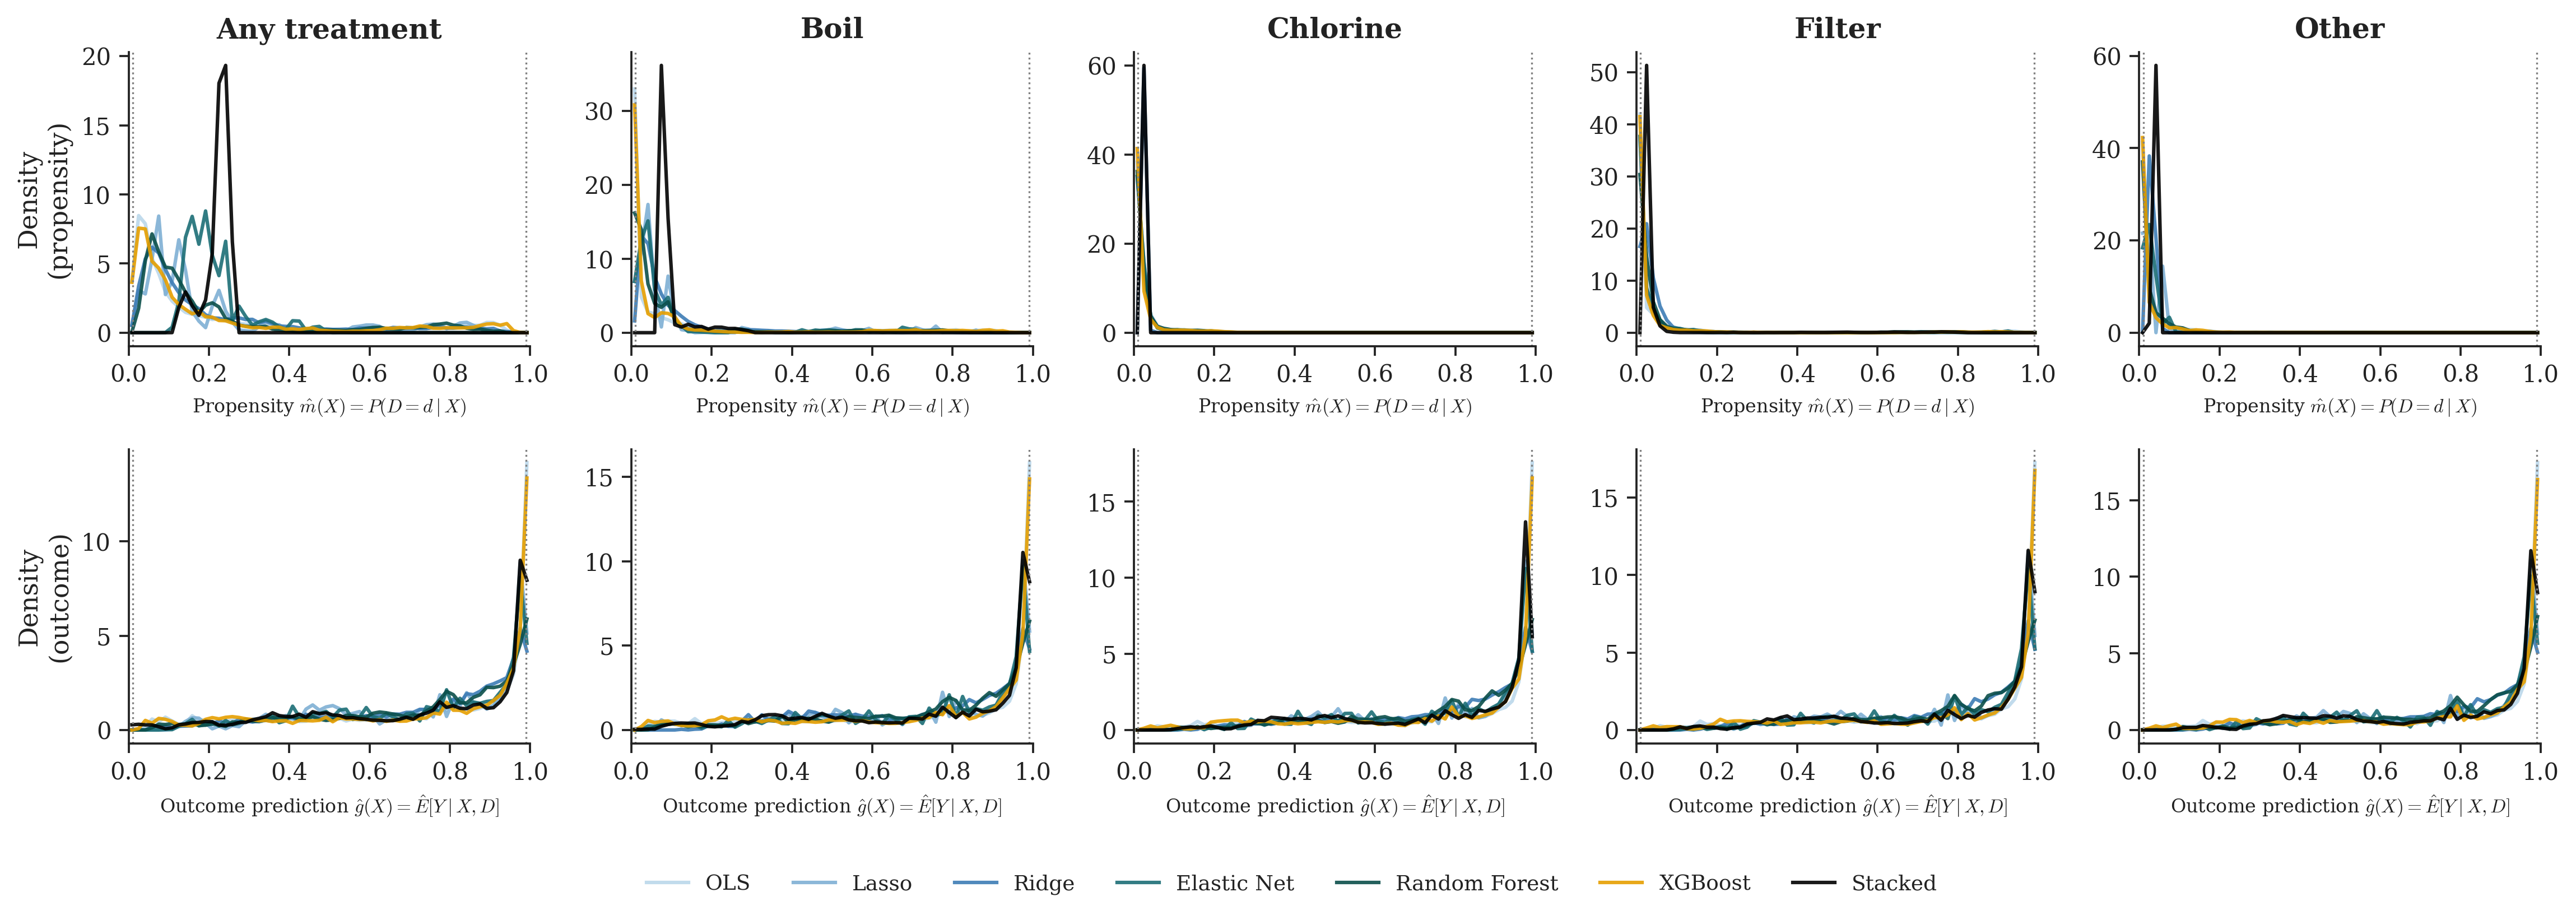
\includegraphics[width=\linewidth]{overlap_HH_SomeRiskHome.png}
{\footnotesize\begin{flushleft} \textit{Notes:} Cross-fitted IRM nuisances by treatment and learner. The any-treatment contrast is the IRM specification used in the main analysis; method-specific IRM diagnostics, where shown, are auxiliary checks only and are not used for the headline method-specific estimates. Top row: propensity $\hat m(X)=P(D{=}d\mid X)$; bottom row: outcome prediction $\hat g(X)=\hat\E[Y\mid X,D]$. Dotted lines mark the $[0.01,0.99]$ trimming bounds; mass at the boundary indicates weak overlap. \end{flushleft}}
\end{figure}

\begin{figure}[htbp]\centering
\caption{Overlap diagnostics (IRM) --- Very High Risk Home E.\,coli ($\geq 101$ CFU)}\label{fig:overlap_irm_vh}
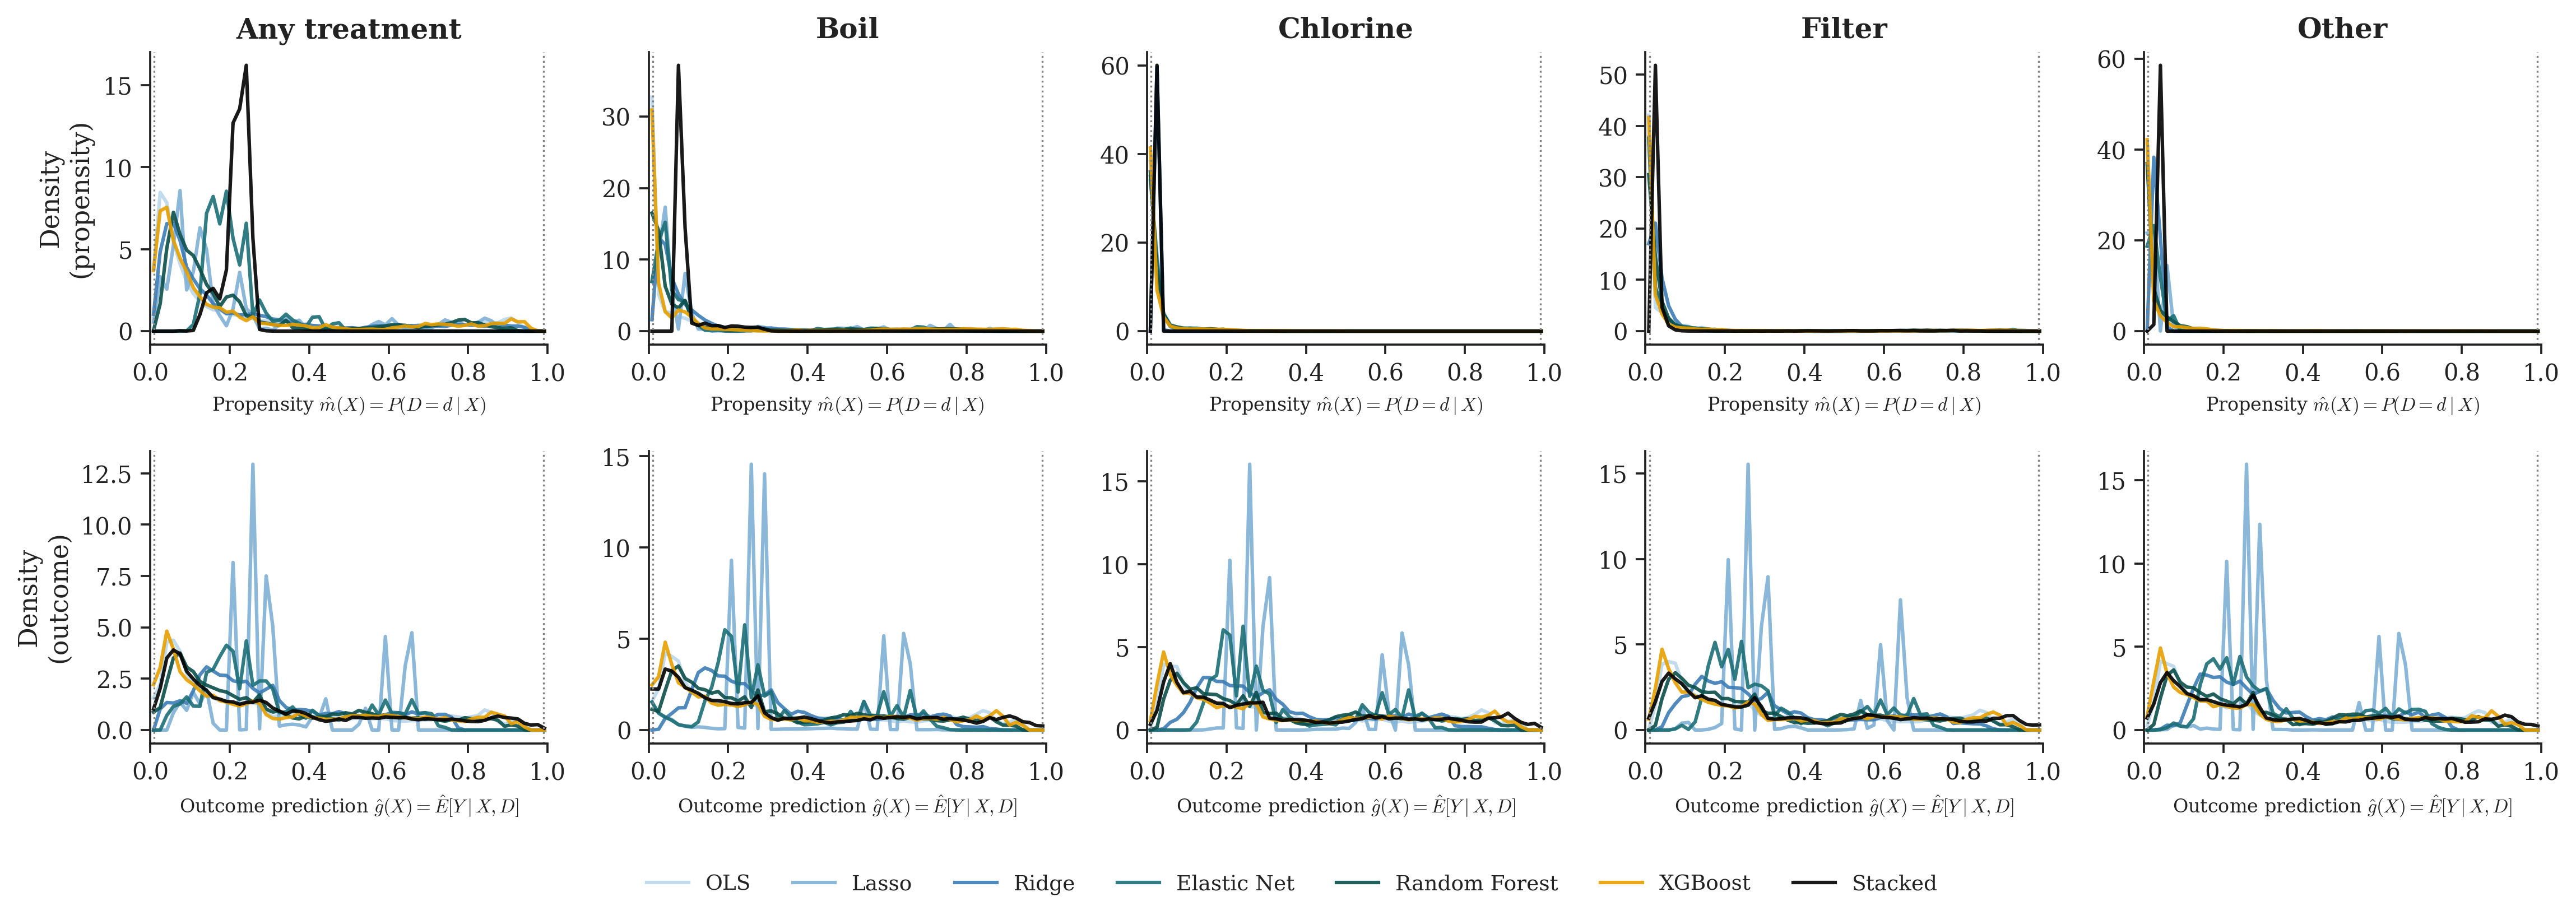
\includegraphics[width=\linewidth]{overlap_HH_VeryHighRiskHome.png}
{\footnotesize\begin{flushleft} \textit{Notes:} As Figure~\ref{fig:overlap_irm}, for the very-high-risk E.\,coli outcome. \end{flushleft}}
\end{figure}

\begin{figure}[htbp]\centering
\caption{Overlap diagnostics (IRM) --- under-five diarrhea}\label{fig:overlap_irm_u5}
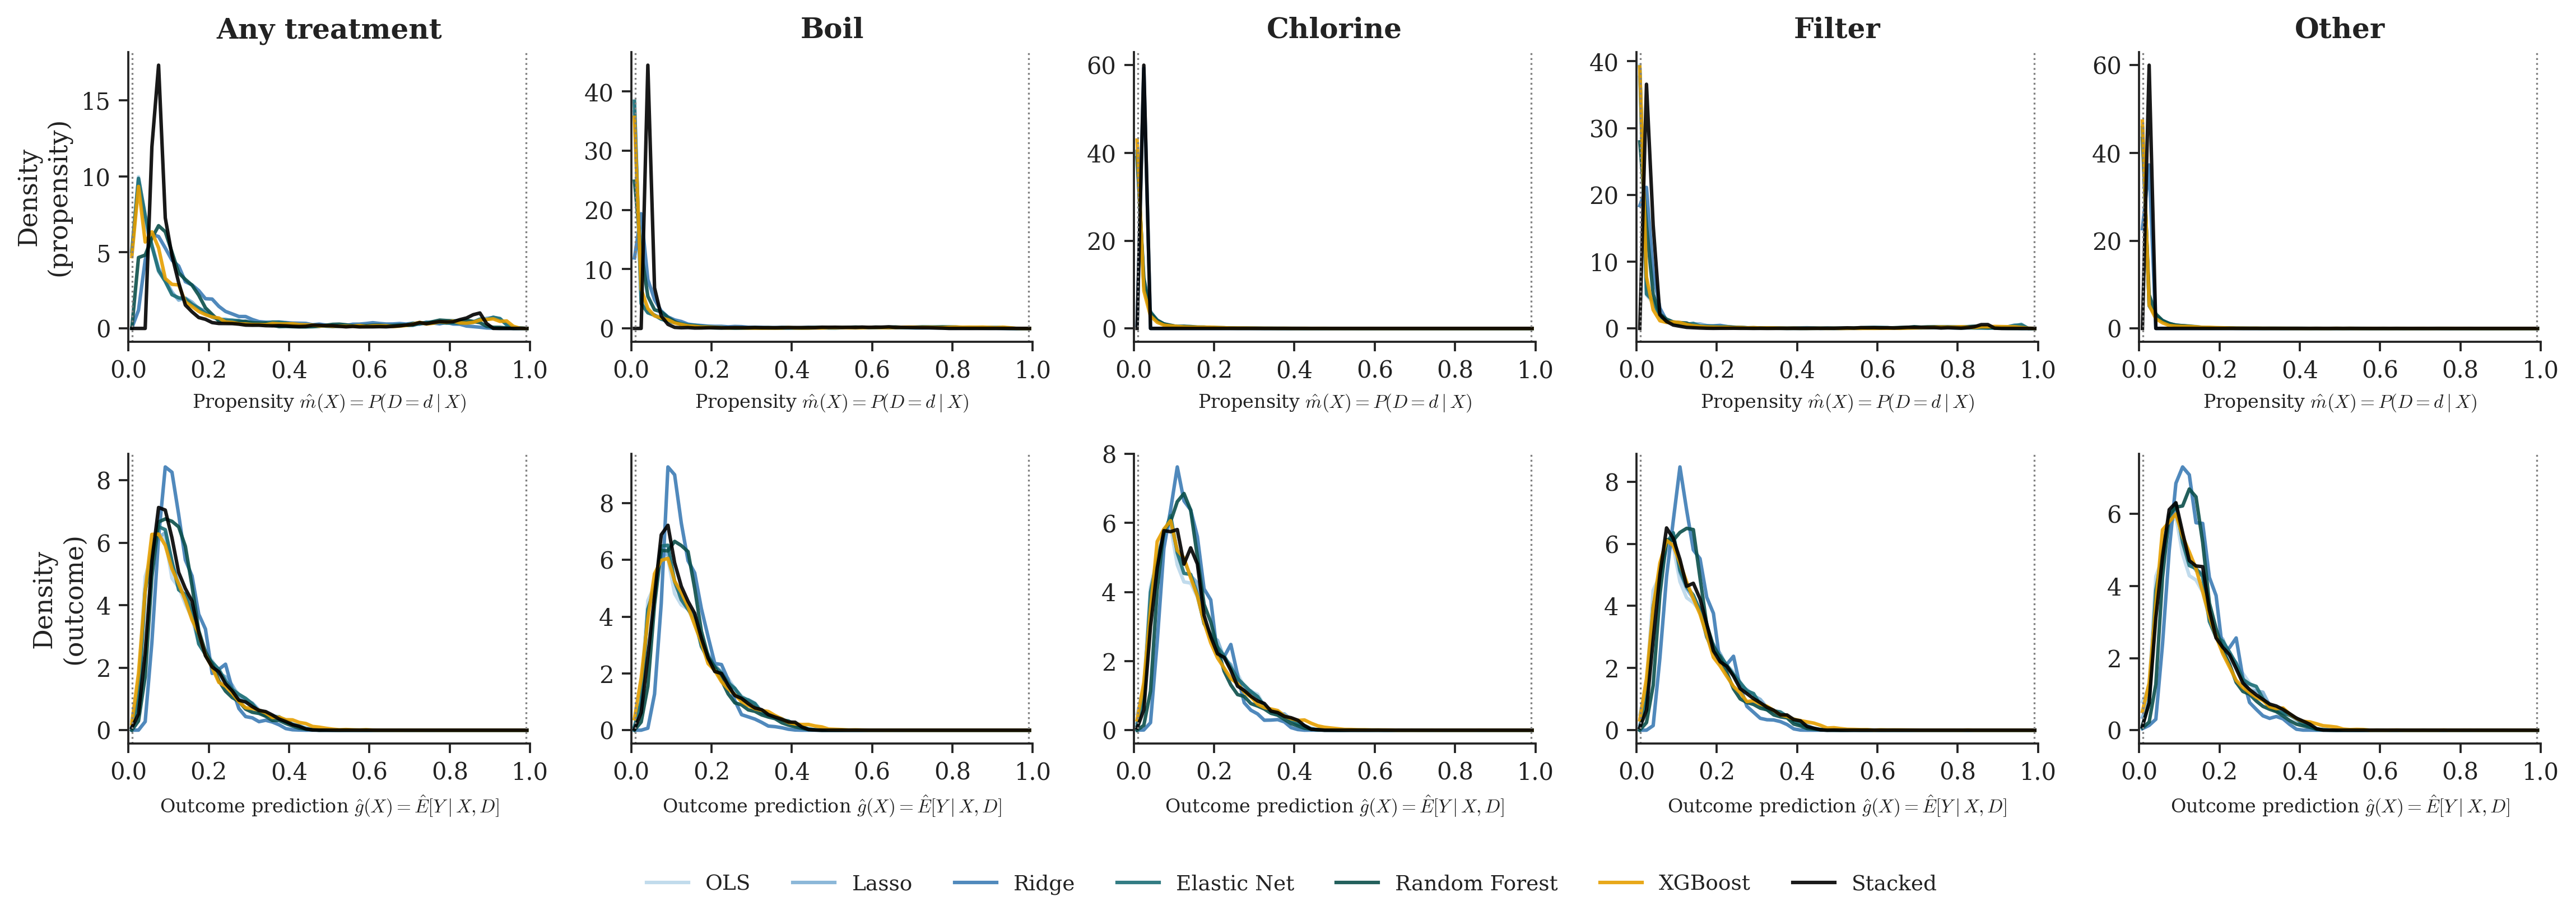
\includegraphics[width=\linewidth]{overlap_U5_diarrhea.png}
{\footnotesize\begin{flushleft} \textit{Notes:} As Figure~\ref{fig:overlap_irm}, for the under-five diarrhea outcome (U5 sample). \end{flushleft}}
\end{figure}

% ---- APOS overlap diagnostics, all three outcomes ----
\begin{figure}[htbp]\centering
\caption{Overlap diagnostics (APOS) --- Some Risk Home E.\,coli}\label{fig:overlap_apos}
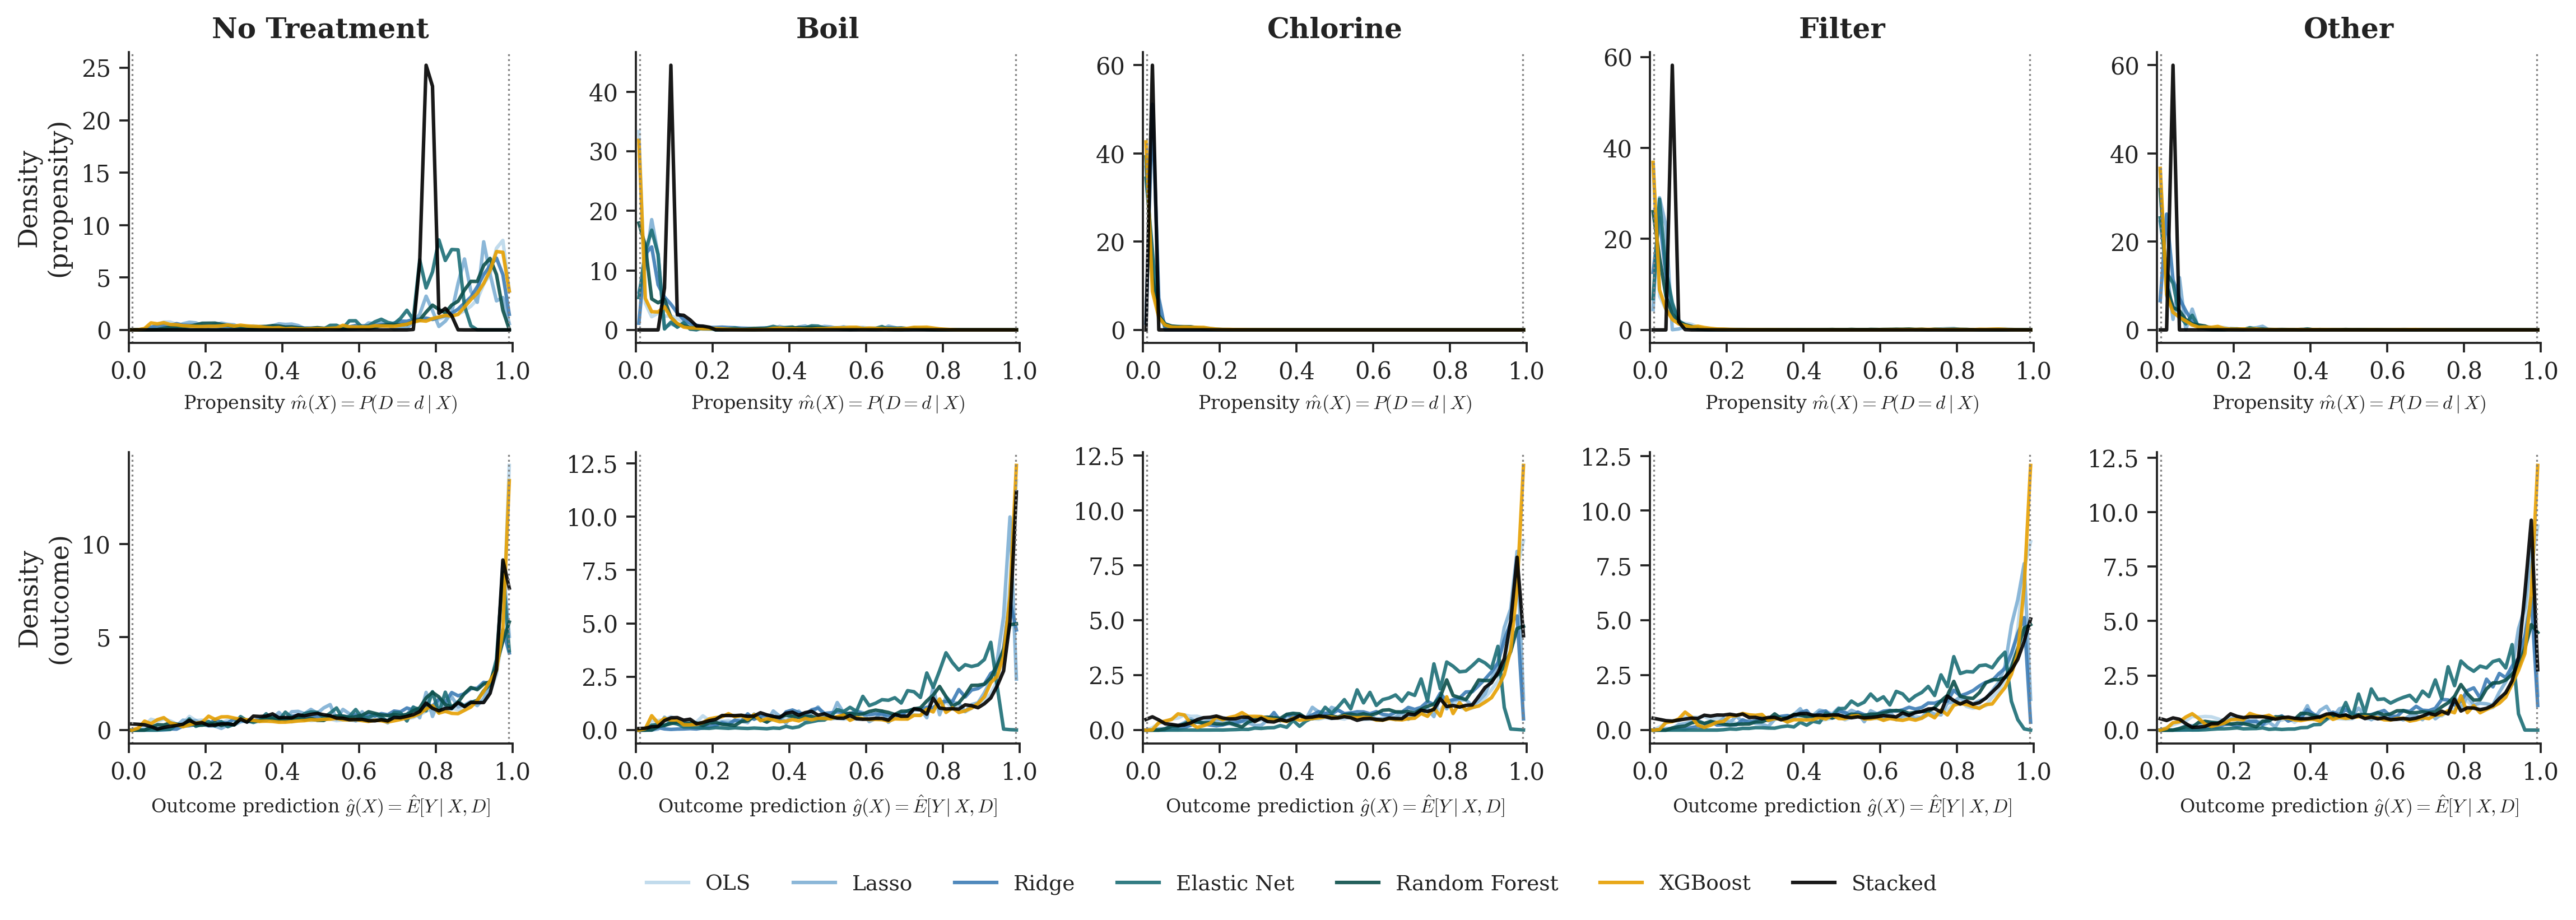
\includegraphics[width=\linewidth]{overlap_apos_HH_SomeRiskHome.png}
{\footnotesize\begin{flushleft} \textit{Notes:} Cross-fitted APOS nuisances by treatment \emph{level} (columns: no treatment and each method, estimated jointly on the full sample with a multinomial propensity) and learner. Top row: per-level propensity $\hat p_d(X)=P(D{=}d\mid X)$; bottom row: outcome prediction $\hat g(X)$. Dotted lines mark the $[0.01,0.99]$ trimming bounds. \end{flushleft}}
\end{figure}

\begin{figure}[htbp]\centering
\caption{Overlap diagnostics (APOS) --- Very High Risk Home E.\,coli ($\geq 101$ CFU)}\label{fig:overlap_apos_vh}
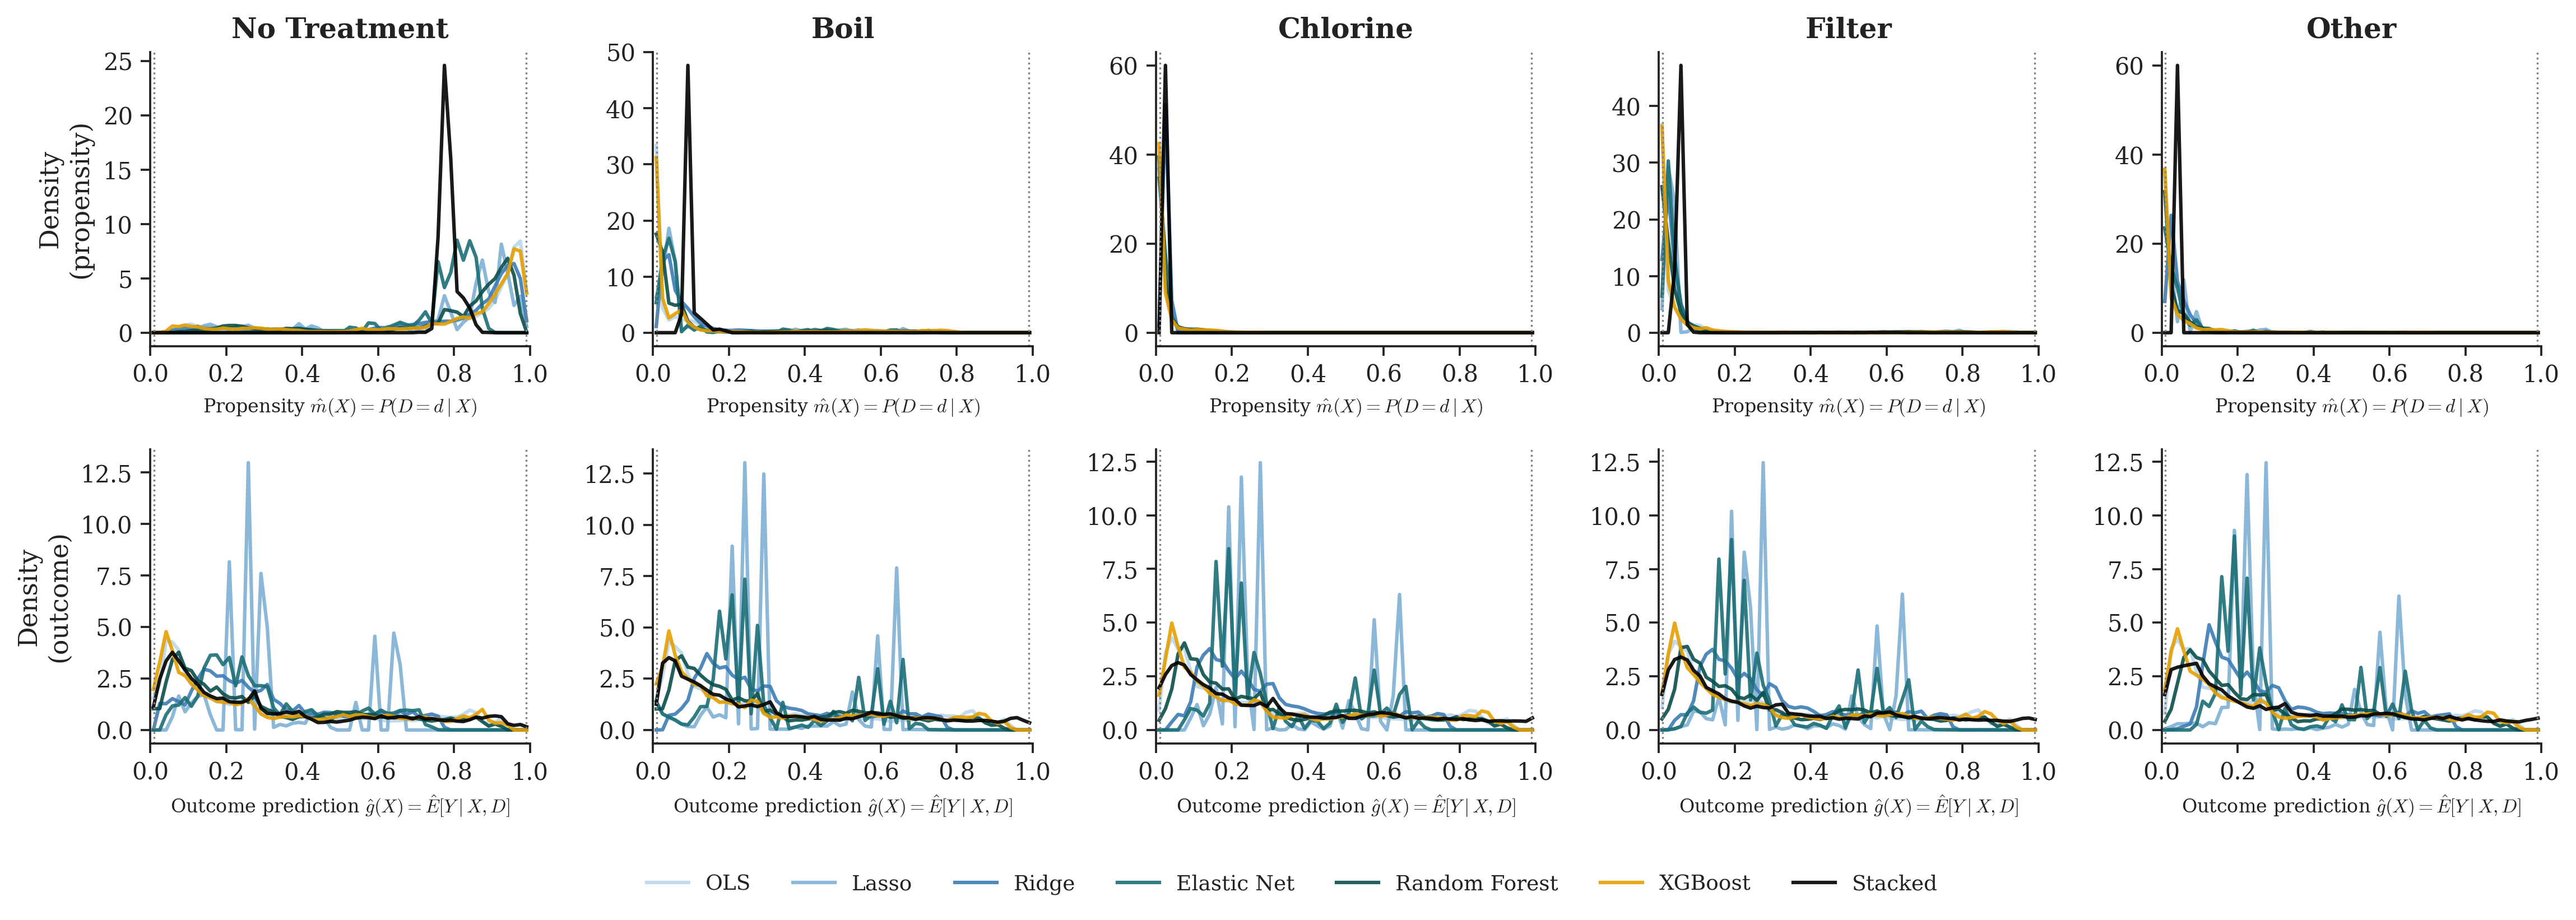
\includegraphics[width=\linewidth]{overlap_apos_HH_VeryHighRiskHome.png}
{\footnotesize\begin{flushleft} \textit{Notes:} As Figure~\ref{fig:overlap_apos}, for the very-high-risk E.\,coli outcome. \end{flushleft}}
\end{figure}

\begin{figure}[htbp]\centering
\caption{Overlap diagnostics (APOS) --- under-five diarrhea}\label{fig:overlap_apos_u5}
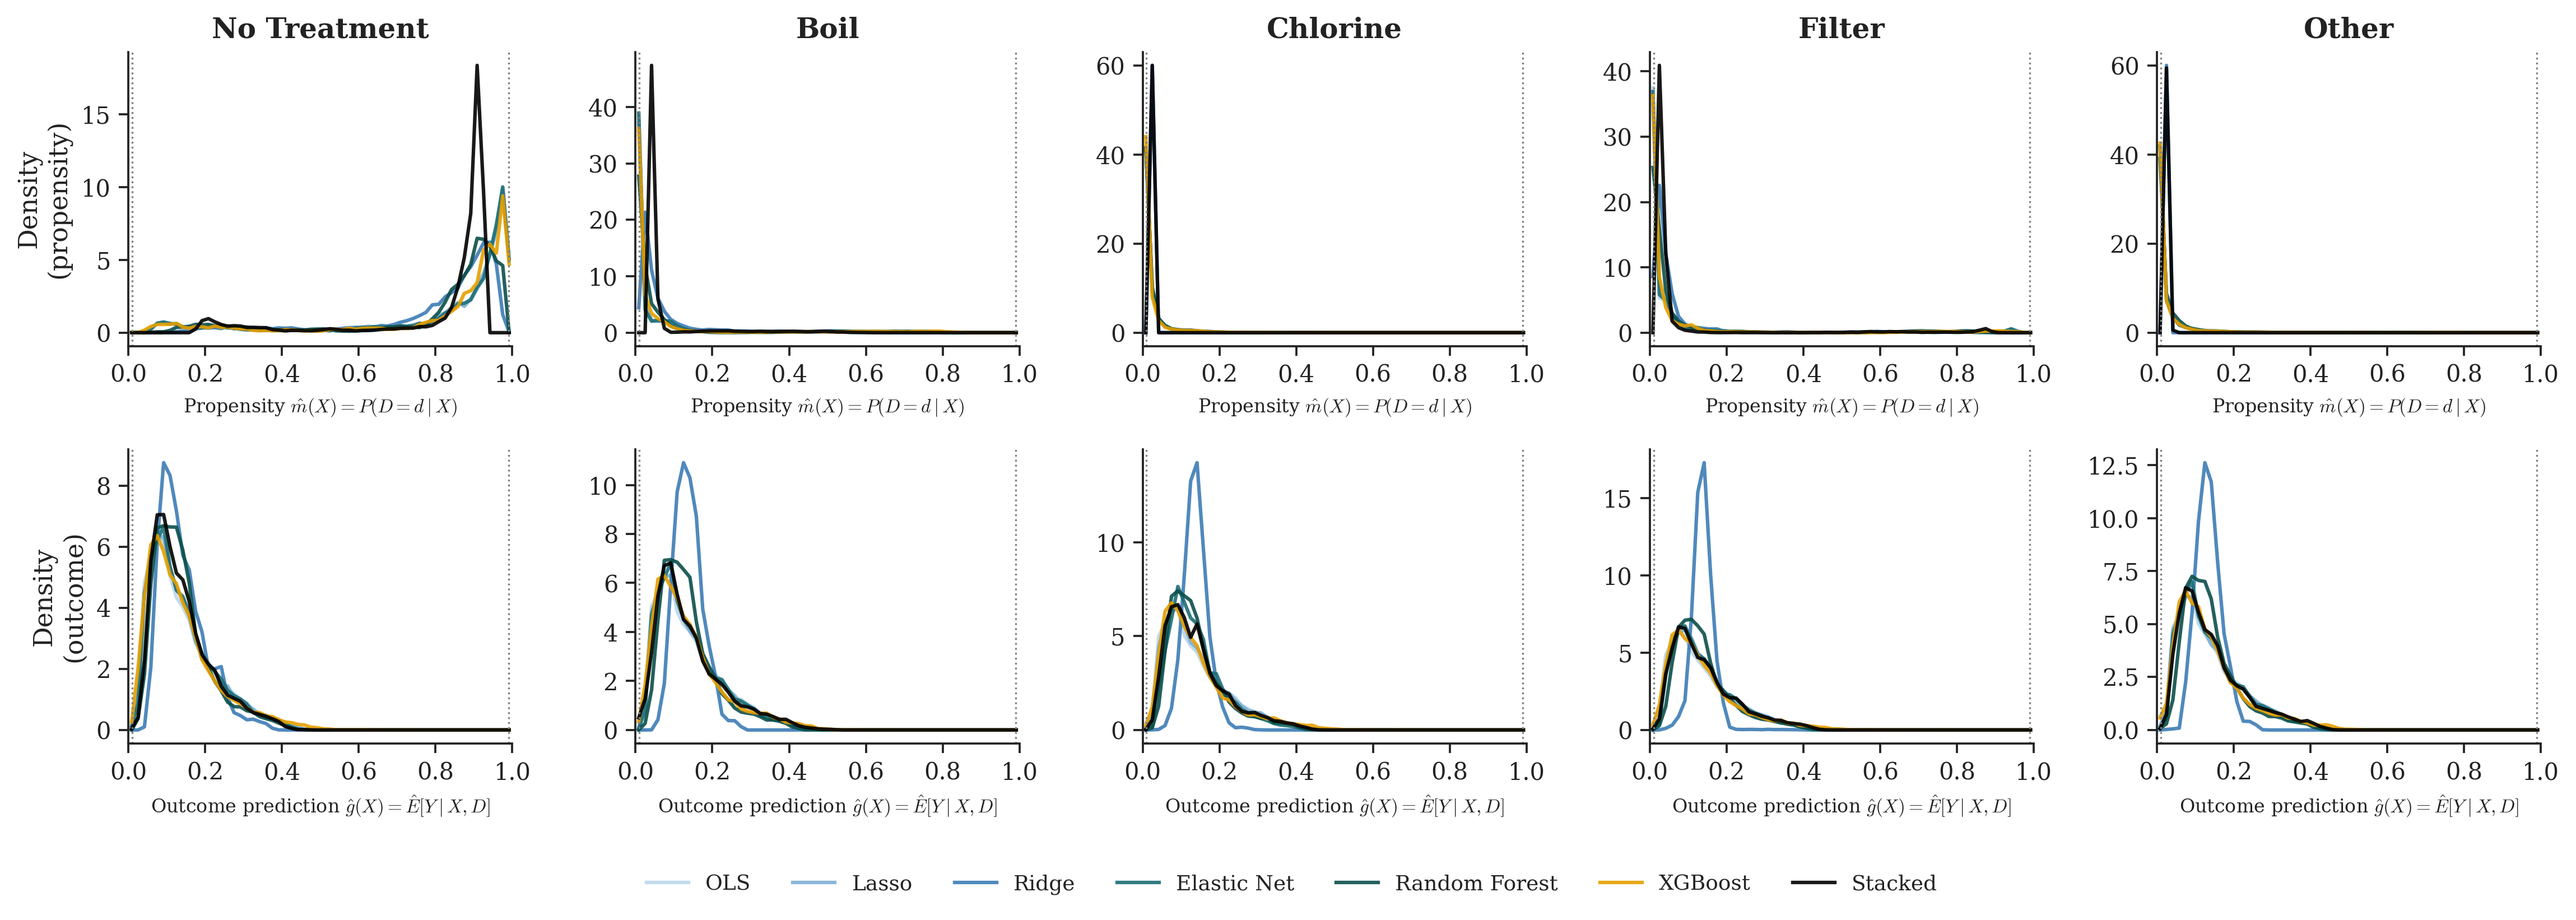
\includegraphics[width=\linewidth]{overlap_apos_U5_diarrhea.png}
{\footnotesize\begin{flushleft} \textit{Notes:} As Figure~\ref{fig:overlap_apos}, for the under-five diarrhea outcome (U5 sample). \end{flushleft}}
\end{figure}




\begin{figure}[htbp]\centering
\caption{Frequency count of treatment and country}\label{ABC}
\begin{subfigure}[b]{0.49\textwidth}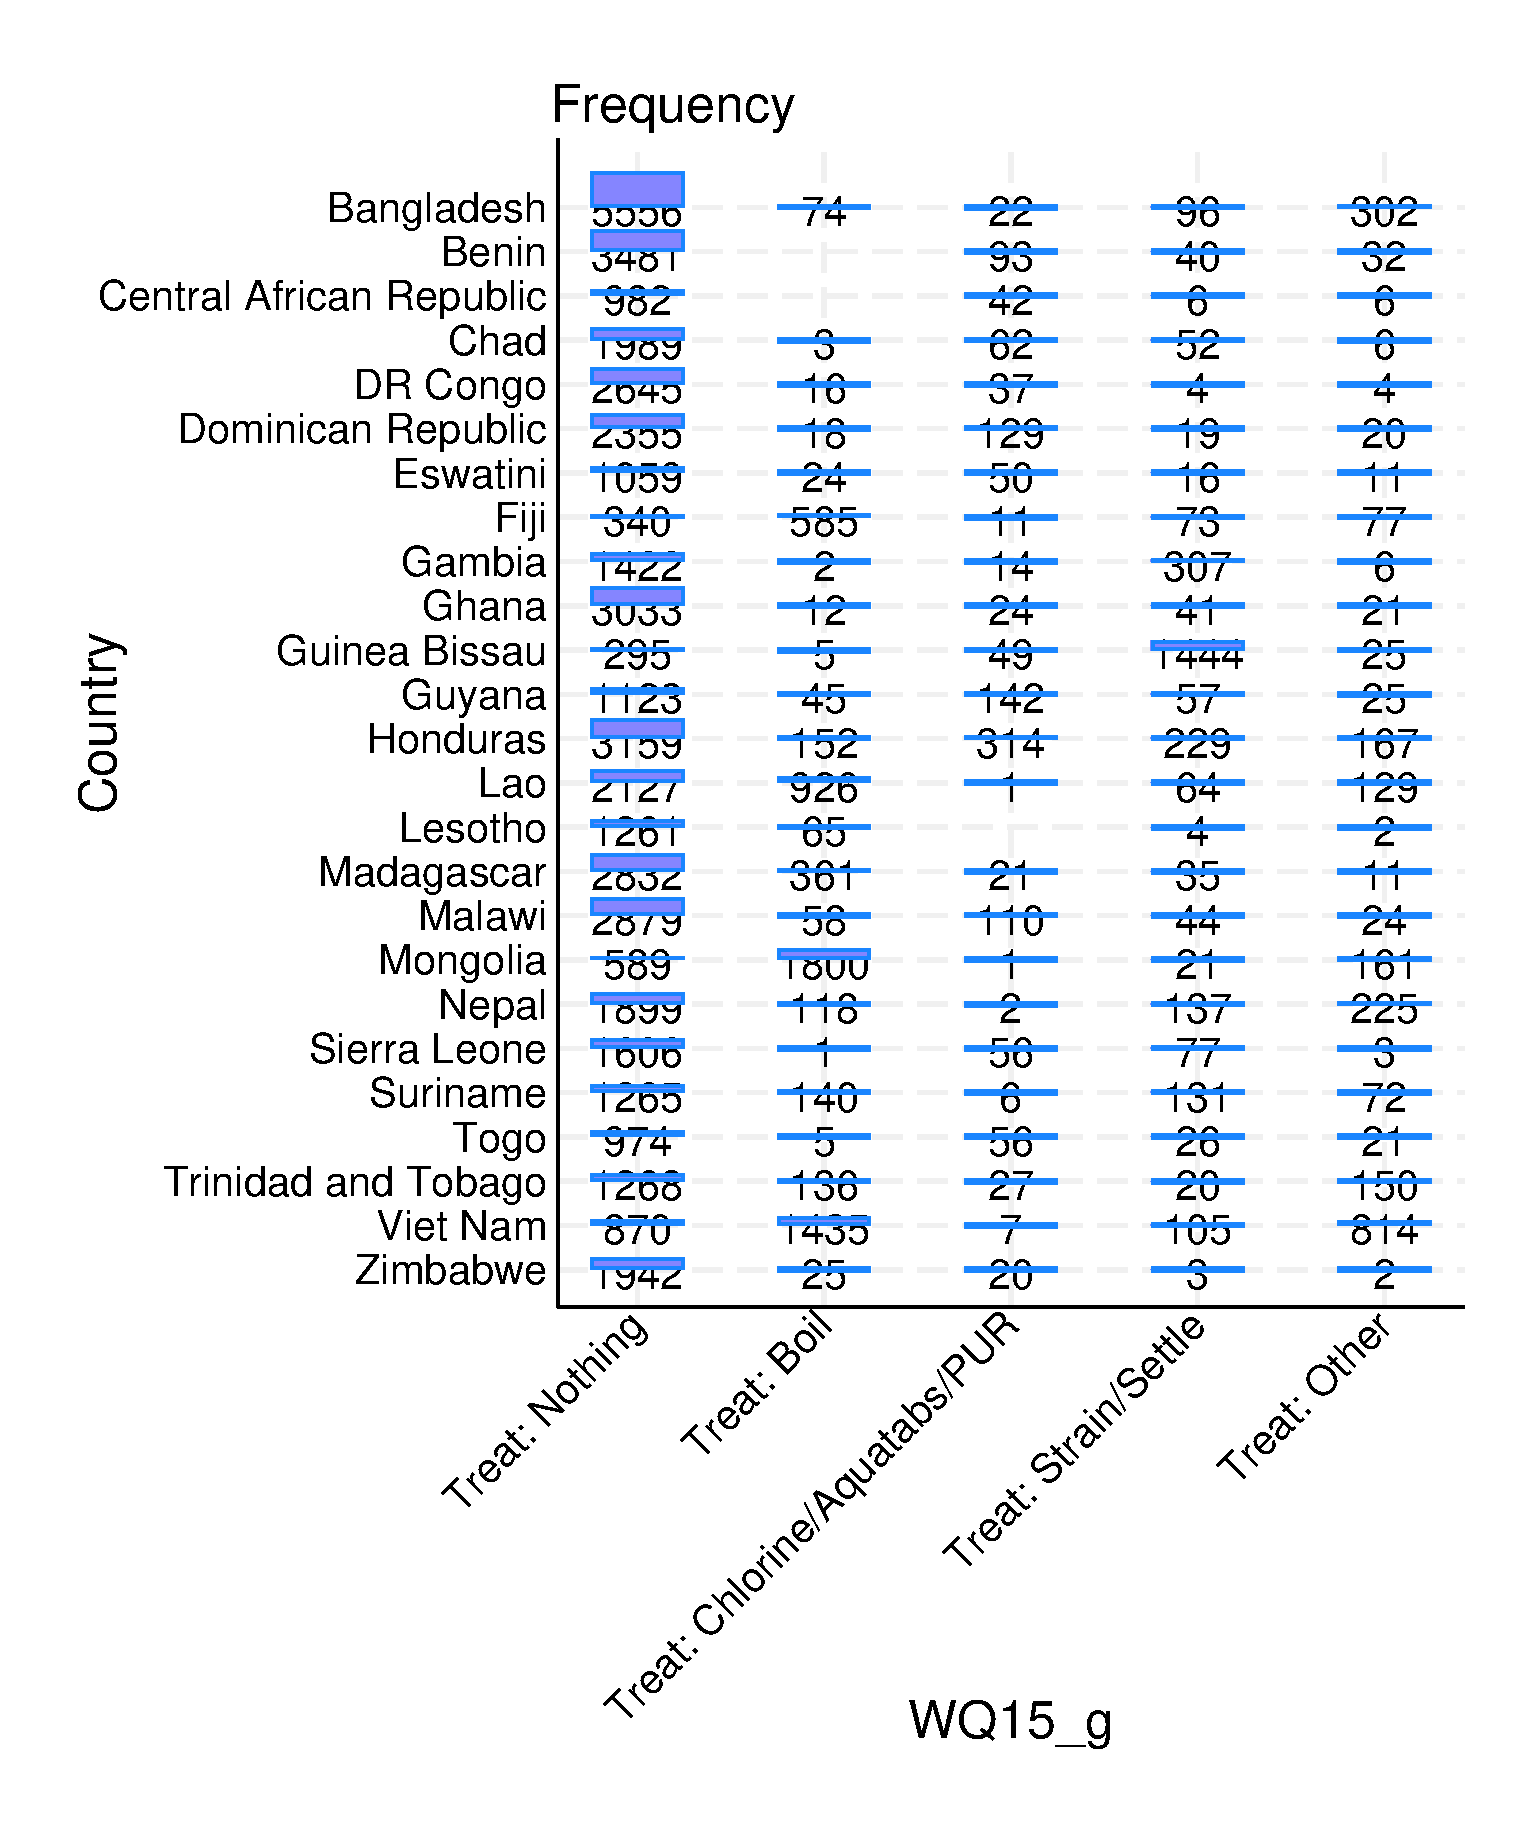
\includegraphics[width=\textwidth]{Freq_Country_Treatment_HH.eps}\end{subfigure}
\begin{subfigure}[b]{0.49\textwidth}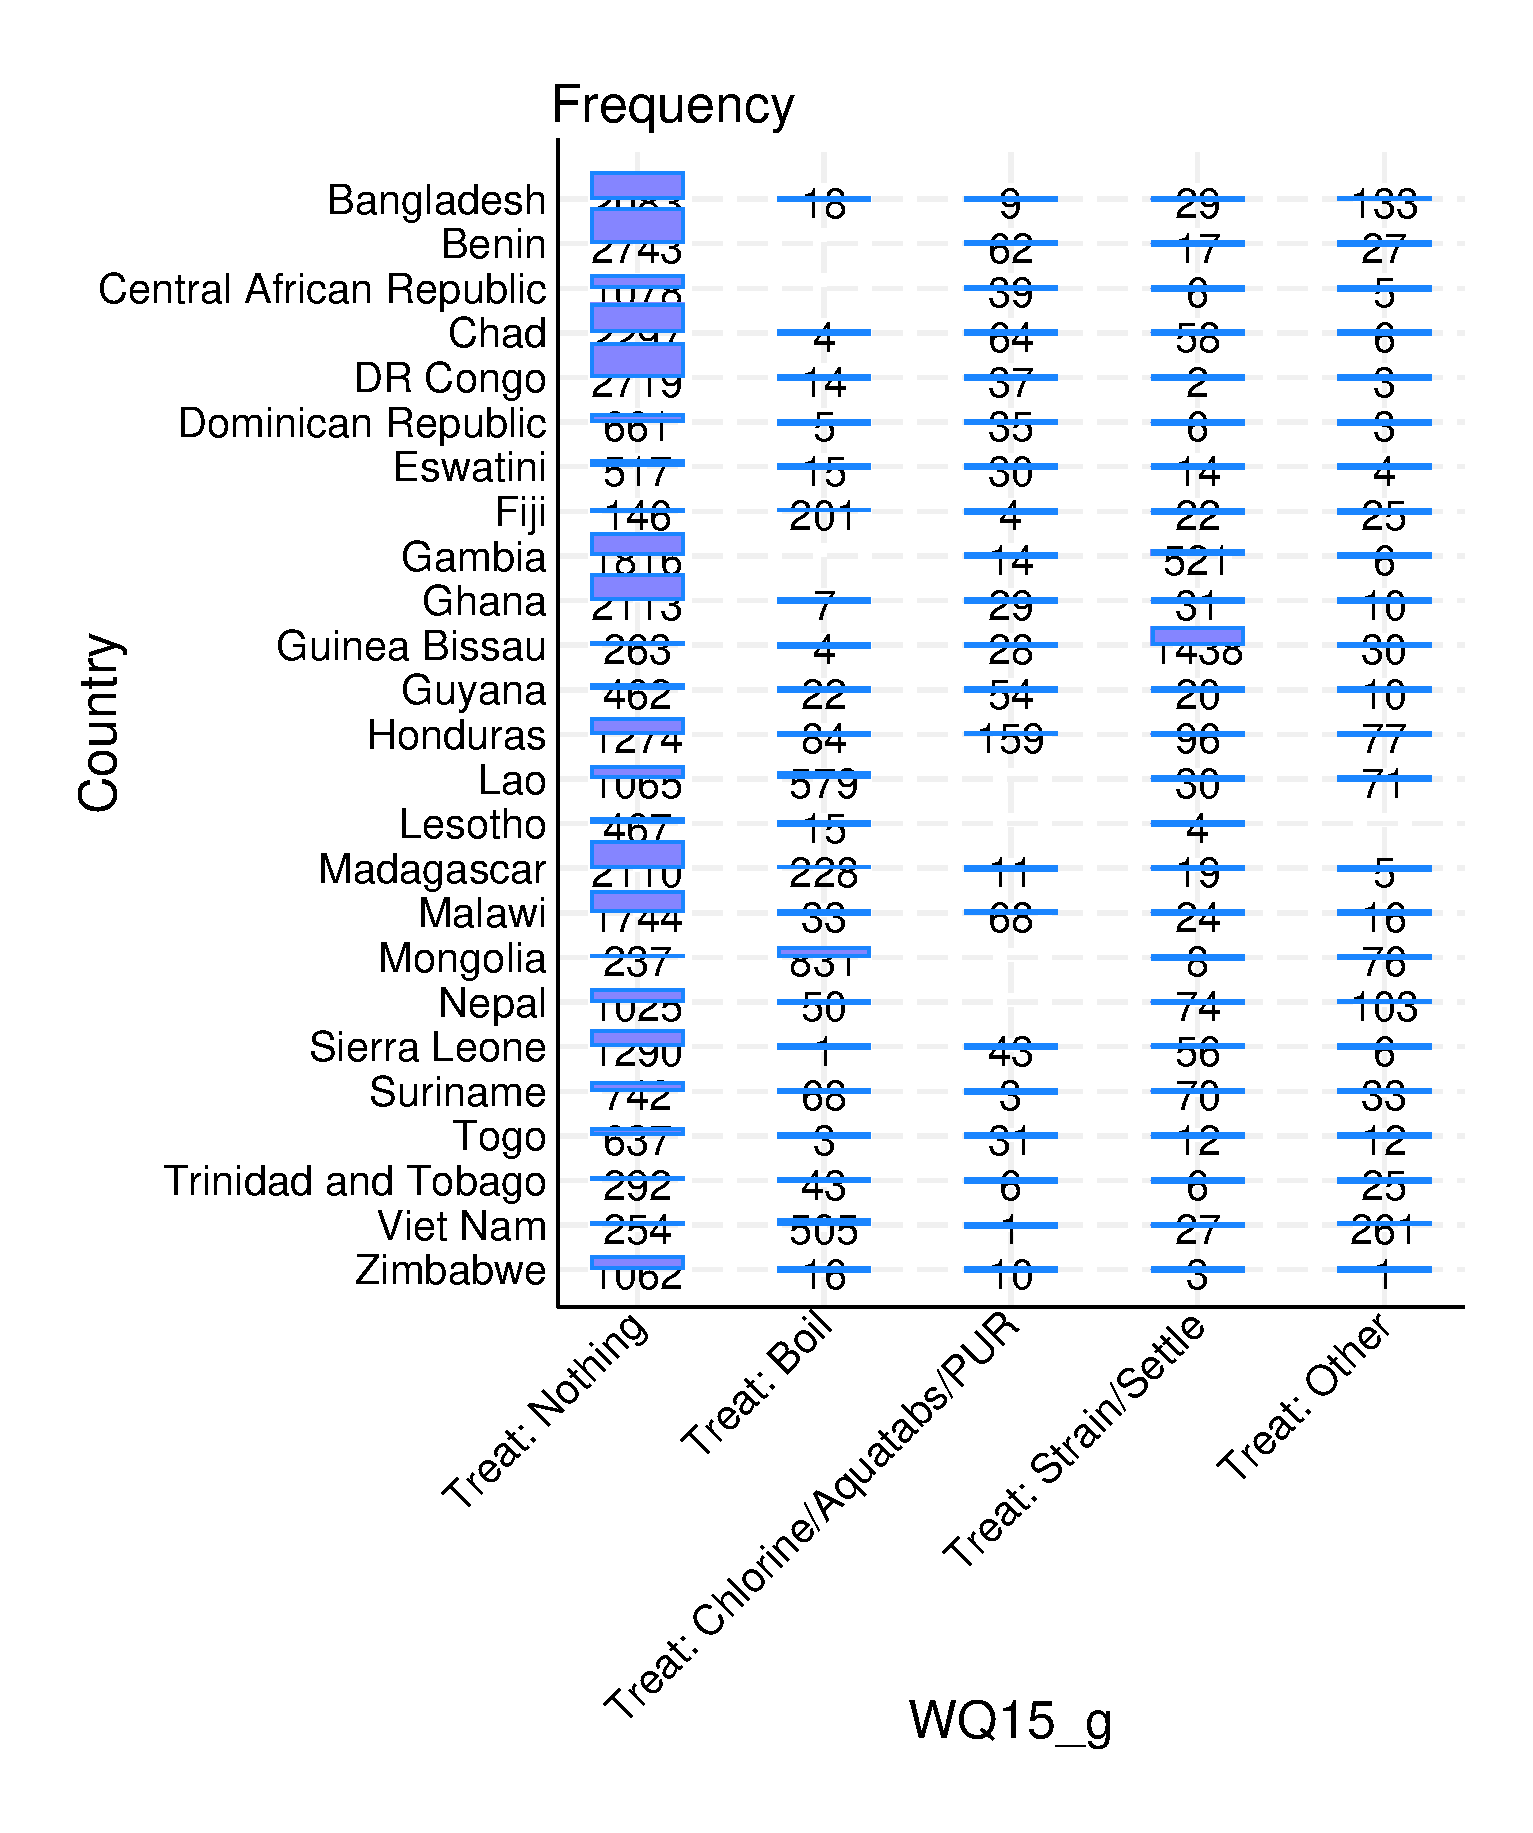
\includegraphics[width=\textwidth]{Freq_Country_Treatment_Child.eps}\end{subfigure}
{\footnotesize  \begin{flushleft} Notes: \end{flushleft}}
\end{figure}

\clearpage
\subsection{Control Variables}
All specifications --- the OLS and the DDML estimators (IRM and APOS) --- use the same control vector, and within DDML it enters both the outcome model and the propensity model. The vector is common to the household E. coli and under-five diarrhea samples; the under-five sample adds two child-level controls, described below.

The household and environmental controls are: (i) household wealth, as four wealth-index quintile indicators (quintiles two through five, relative to the poorest); (ii) education of the household head, as indicators for primary and for secondary-or-higher education together with a missing-value category, relative to no education; (iii) urban versus rural residence; (iv) the main drinking-water source, as grouped MICS categories (piped supply, tube well or borehole, protected and unprotected wells and springs, surface and rainwater, packaged water, and other); (v) sanitation, as indicators for pit latrine, open defecation, and a missing category, relative to a flush toilet; (vi) household composition, as indicators for the presence of any under-five child, of a girl under fifteen, and of a boy under fifteen; and (vii) the contamination of the household's source water, as deciles of the source-water E. coli test (CFU per 100\,ml).

Country fixed effects (one indicator per country) absorb cross-country heterogeneity in baseline contamination risk, infrastructure, climate, and public-health environment. Within the interactive (IRM) and potential-outcome (APOS) frameworks these indicators also let treatment effects vary across country contexts, where the effectiveness of household treatment may depend on local environmental and institutional conditions.

For the under-five (diarrhea) sample the control vector is augmented with two child-level variables: the child's age in years and the child's sex. No other controls differ between the two samples.

Two source-water variables warrant comment. The decile measure above enters every model as a confounder: source contamination is measured upstream of the household's point-of-use treatment decision and plausibly drives both whether a household treats and the health outcome, so it is a pre-treatment confounder rather than a mediator. A separate, coarser categorisation of source risk (no risk, moderate, very high) is not used as a control; it instead serves as the dimension along which we examine treatment-effect heterogeneity, since point-of-use treatment is expected to matter little when source water is clean and more when it is contaminated. The household's number of under-five children is likewise not a control --- household composition is captured by the indicators in~(vi), and the child count is reserved as a moderator in the heterogeneity analysis.

\section{Empirical Results}\label{Empirical}
This section presents ordinary least squares (OLS) estimates as a benchmark, followed by DDML estimates from the any-treatment IRM and the method-specific APOS specifications.

\subsection{Characteristics Associated with Water Treatment}\label{Lasso}

Before estimating treatment effects, we examine the characteristics associated with adoption of any household water treatment. Table~\ref{tab:treatment_predictors} reports a logistic regression (signed log-odds), penalised-logit selection (Lasso and Elastic Net), and tree-based variable importance (random forest and XGBoost). Every model includes country fixed effects, and the covariates are ordered by their mean random-forest/XGBoost importance. Adoption is strongly patterned. It rises with household wealth (top-quintile log-odds $+0.93$ relative to the poorest), with the education of the household head, and with source-water E.\,coli deciles. Households facing dirtier source water are more likely to treat, although the strongest predictors are the middle source-water deciles (5--8), not the most contaminated deciles (9--10). This pattern suggests that households facing the dirtiest source water often do not, or cannot, treat it. Adoption is lower among households relying on packaged or bottled water and among households with poorer sanitation. The five learners agree on the main predictors and predict adoption well (AUC $\approx 0.86$--$0.90$). These wealth, sanitation, and source-contamination gradients are precisely the forms of confounding that the DDML adjustment is designed to remove.

% Requires: \usepackage{booktabs}
\begin{table}[htbp]
\centering
\caption{Characteristics associated with water-treatment adoption}
\label{tab:treatment-predictors}
\small\setlength{\tabcolsep}{5pt}
\begin{tabular}{lccccc}
\toprule
Covariate & Logit & Lasso & E.\,net & RF & XGB \\
 & (log-odds) & \multicolumn{2}{c}{(penalized coef.)} & \multicolumn{2}{c}{(importance $\times100$)} \\
\cmidrule(lr){3-4}\cmidrule(lr){5-6}
\midrule
Packaged/bottled \textit{(Water source)} & -2.73*** & -1.95 & -1.78 & 6.5 & 4.4 \\
Missing \textit{(Education (head))} & +0.46*** & +0.00 & +0.40 & 3.0 & 2.1 \\
Tube/well/borehole \textit{(Water source)} & -0.36*** & -0.55 & -0.55 & 2.3 & 1.5 \\
Protected well/spring \textit{(Water source)} & +0.58*** & +0.16 & +0.32 & 2.1 & 0.7 \\
Pit Latrine \textit{(Sanitation)} & -0.15*** & -0.55 & -0.46 & 1.9 & 0.8 \\
Open Defecation \textit{(Sanitation)} & -0.58*** & -0.82 & -0.72 & 1.4 & 1.2 \\
Other \textit{(Water source)} & +0.03 & +0.00 & +0.00 & 1.1 & 0.8 \\
Decile 8 \textit{(Source E.\,coli)} & +0.59*** & +0.19 & +0.25 & 0.9 & 0.3 \\
Q5 (vs Q1) \textit{(Wealth quintile)} & +0.92*** & +0.04 & +0.08 & 0.7 & 0.4 \\
Secondary or higher \textit{(Education (head))} & +0.29*** & +0.08 & +0.17 & 0.8 & 0.3 \\
Surface/rain \textit{(Water source)} & +0.25*** & +0.00 & +0.00 & 0.7 & 0.4 \\
Unprotected well/spring \textit{(Water source)} & +0.39*** & +0.00 & +0.00 & 0.6 & 0.3 \\
Urban \textit{(Residence)} & -0.05 & +0.00 & +0.00 & 0.6 & 0.2 \\
Q4 (vs Q1) \textit{(Wealth quintile)} & +0.44*** & +0.00 & +0.00 & 0.4 & 0.2 \\
Q2 (vs Q1) \textit{(Wealth quintile)} & +0.10** & +0.00 & +0.00 & 0.4 & 0.2 \\
Decile 7 \textit{(Source E.\,coli)} & +0.42*** & +0.00 & +0.06 & 0.2 & 0.2 \\
Primary \textit{(Education (head))} & +0.12*** & +0.00 & +0.00 & 0.3 & 0.1 \\
Any under-5 child \textit{(Household composition)} & +0.02 & +0.00 & -0.00 & 0.3 & 0.1 \\
Q3 (vs Q1) \textit{(Wealth quintile)} & +0.28*** & +0.00 & +0.00 & 0.3 & 0.1 \\
Missing \textit{(Sanitation)} & -0.10 & +0.00 & +0.00 & 0.1 & 0.2 \\
Decile 6 \textit{(Source E.\,coli)} & +0.32*** & +0.00 & +0.00 & 0.2 & 0.1 \\
Girl aged $<15$ \textit{(Household composition)} & -0.08 & +0.00 & +0.00 & 0.1 & 0.1 \\
Decile 5 \textit{(Source E.\,coli)} & +0.24*** & +0.00 & +0.00 & 0.1 & 0.1 \\
Boy aged $\leq15$ \textit{(Household composition)} & -0.20 & +0.00 & +0.00 & 0.0 & 0.2 \\
\bottomrule
\end{tabular}
\par\vspace{3pt}
\begin{minipage}{\linewidth}\footnotesize \textit{Notes:} Outcome is any household water treatment ($N=59,620$, adoption rate $0.212$). Rows are ordered by mean random-forest/XGBoost importance. All models include country fixed effects, which are omitted from the table. Reference categories are Q1 for wealth, no education, flush toilet, piped water, and rural residence. Logit reports signed log-odds; lasso and elastic net report penalized coefficients; RF and XGB report feature importance. $^{***}p<0.01$, $^{**}p<0.05$, $^{*}p<0.10$.\end{minipage}
\end{table}


\subsection{Water Treatment Effect on E. coli}\label{OLS}

Tables \ref{tab:Est_EColi_OLS_SomeRiskHome_full} and \ref{tab:Est_EColi_OLS_VeryHighRiskHome_full} present ordinary least squares (OLS) estimates of the association between household water treatment and E. coli contamination in household drinking water, using the same set of control variables and stratifying households by the level of E. coli risk at the water source.

Table \ref{tab:Est_EColi_OLS_SomeRiskHome_full} examines the probability that household drinking water contains any detectable E.\,coli. Compared with the unconditional estimates in Panel A, the coefficients in Panel B remain negative but are smaller in magnitude, suggesting that observable controls absorb part of the upward bias in the simple correlation. The specification with basic controls indicates that household water treatment is associated with a 9.4 percentage-point reduction in the probability of detecting E.\,coli. Given that 78 percent of households in the sample have detectable E.\,coli in drinking water, this estimate implies a substantial reduction in contamination risk associated with water treatment.

Among households with no detectable E.\,coli at the source, 23,595 households are included in the sample, yet approximately 50 percent exhibit some E.\,coli contamination at the point of use. Water treatment is associated with a statistically significant 7.3 percentage-point reduction in the probability of E.\,coli detection. The estimated reduction is larger among households whose source water contains moderate contamination levels (1--100 CFU). In contrast, the estimated effects are smaller for households facing high-risk source contamination, potentially reflecting recontamination during storage, inconsistent treatment, or lower chlorine effectiveness under high organic load or incorrect dosing.


%-------------------------------------------------------------%
{\renewcommand\normalsize{\small}\normalsize\singlespacing  
\input{Table/Est_EColi_OLS_SomeRiskHome_full.tex}
}  
%-------------------------------------------------------------% 

Table \ref{tab:Est_EColi_OLS_VeryHighRiskHome_full} examines the probability that household drinking water contains very high E.\,coli contamination (greater than 100 CFU). Overall, water treatment does not significantly reduce the probability of very high contamination among households whose source water is classified as low risk. This is partly mechanical: only about 14 percent of these households exhibit very high point-of-use contamination, leaving limited scope for detectable treatment effects. The estimated association becomes larger in magnitude as source contamination risk increases, suggesting that treatment effectiveness is more visible when households face higher baseline microbial risk at the source.

%-------------------------------------------------------------%
{\renewcommand\normalsize{\small}\normalsize\singlespacing  
\input{Table/Est_EColi_OLS_VeryHighRiskHome_full.tex}}  
%-------------------------------------------------------------% 


Table~\ref{tab:results-ecoli} reports the DDML estimates of household water treatment on E.\,coli contamination at the point of use. The any-treatment IRM estimates show a clear reduction in contamination. In the preferred stacked specification, any household water treatment lowers the probability of any detectable E.\,coli by 8.5 percentage points, relative to an outcome mean of 73.7 percent, and lowers the probability of very high contamination by 7.1 percentage points, relative to a mean of 30.8 percent. The estimates are statistically significant across all nuisance learners and are close in magnitude across specifications, indicating that the result is not driven by a particular machine-learning model.

The APOS contrasts show substantial differences by treatment method. Boiling produces the largest and most consistent reduction: in the stacked specification, it lowers any detectable E.\,coli by 16.2 percentage points and very high contamination by 10.6 percentage points. Chlorination also reduces contamination, but the estimated effect is smaller, at 3.3 percentage points for any detectable E.\,coli and 4.0 percentage points for very high contamination. Filtering does not reduce any detectable E.\,coli in the stacked specification and only reduces very high contamination by 3.3 percentage points. The ``other'' category is large and negative for both outcomes, but because it pools heterogeneous practices, it should be interpreted as an aggregate residual category rather than as a single treatment mechanism. Overall, the DDML estimates support a strong water-quality result: household treatment reduces measured E.\,coli contamination, with the clearest method-specific evidence for boiling and more modest evidence for chlorination.

%-------------------------------------------------------------%
{\renewcommand\normalsize{\small}\normalsize\singlespacing
% Requires: \usepackage{booktabs, pdflscape, graphicx, adjustbox}
\begin{landscape}
\begin{table}[htbp]
\centering
\caption{DDML estimates: Water treatment and household E.coli contamination}
\label{tab:results-ecoli}
\scriptsize
\setlength{\tabcolsep}{3pt}
\renewcommand{\arraystretch}{0.94}
\begin{adjustbox}{max width=\linewidth, max totalheight=0.70\textwidth, center}
\begin{tabular}{l|ccccccc|ccccccc}
\toprule
 & \multicolumn{7}{c|}{Some Risk Home (E.coli 1--100 CFU)} & \multicolumn{7}{c}{Very High Risk Home (E.coli $\geq$ 101 CFU)} \\
\cmidrule(lr){2-8} \cmidrule(lr){9-15}
 & OLS & Lasso & Ridge & Elastic Net & Random Forest & XGBoost & Stacked & OLS & Lasso & Ridge & Elastic Net & Random Forest & XGBoost & Stacked \\
\midrule
Any Treatment & -0.025*** & -0.023*** & -0.023*** & -0.022*** & -0.008 & -0.013* & -0.019*** & -0.061*** & -0.069*** & -0.070*** & -0.072*** & -0.066*** & -0.071*** & -0.070*** \\
 & (0.009) & (0.006) & (0.004) & (0.004) & (0.005) & (0.008) & (0.005) & (0.008) & (0.005) & (0.003) & (0.003) & (0.004) & (0.006) & (0.006) \\
\quad RV & 0.01 & 0.01 & 0.02 & 0.02 & 0.00 & 0.01 & 0.01 & 0.04 & 0.05 & 0.06 & 0.06 & 0.04 & 0.04 & 0.04 \\
\quad RV$_\alpha$ & 0.00 & 0.01 & 0.01 & 0.01 & 0.00 & 0.00 & 0.01 & 0.03 & 0.04 & 0.06 & 0.06 & 0.04 & 0.03 & 0.03 \\
\quad $N$ & \multicolumn{7}{c|}{59,620} & \multicolumn{7}{c}{59,620} \\
\midrule
Boil & -0.009 & -0.040*** & -0.020*** & -0.039*** & -0.041*** & -0.029*** & -0.035*** & -0.103*** & -0.111*** & -0.108*** & -0.111*** & -0.100*** & -0.104*** & -0.106*** \\
 & (0.012) & (0.007) & (0.006) & (0.007) & (0.007) & (0.010) & (0.006) & (0.009) & (0.006) & (0.005) & (0.005) & (0.006) & (0.008) & (0.005) \\
\quad RV & 0.00 & 0.01 & 0.01 & 0.01 & 0.01 & 0.01 & 0.02 & 0.03 & 0.04 & 0.04 & 0.04 & 0.03 & 0.03 & 0.08 \\
\quad RV$_\alpha$ & 0.00 & 0.01 & 0.00 & 0.01 & 0.01 & 0.00 & 0.02 & 0.02 & 0.04 & 0.04 & 0.04 & 0.03 & 0.02 & 0.07 \\
\quad $N$ & \multicolumn{7}{c|}{59,620} & \multicolumn{7}{c}{59,620} \\
\midrule
Chlorine & 0.025* & 0.018 & 0.027** & 0.018 & 0.008 & 0.021 & 0.005 & -0.063*** & -0.060*** & -0.065*** & -0.057*** & -0.065*** & -0.061*** & -0.027** \\
 & (0.013) & (0.012) & (0.012) & (0.012) & (0.011) & (0.013) & (0.013) & (0.010) & (0.010) & (0.010) & (0.010) & (0.009) & (0.011) & (0.011) \\
\quad RV & 0.01 & 0.00 & 0.01 & 0.00 & 0.00 & 0.00 & 0.00 & 0.02 & 0.02 & 0.02 & 0.02 & 0.02 & 0.02 & 0.01 \\
\quad RV$_\alpha$ & 0.00 & 0.00 & 0.00 & 0.00 & 0.00 & 0.00 & 0.00 & 0.01 & 0.01 & 0.01 & 0.01 & 0.01 & 0.01 & 0.00 \\
\quad $N$ & \multicolumn{7}{c|}{59,620} & \multicolumn{7}{c}{59,620} \\
\midrule
Filter & -0.003 & 0.038*** & 0.022*** & 0.039*** & -0.006 & -0.006 & 0.047*** & -0.017 & -0.031*** & -0.026*** & -0.031*** & -0.017* & -0.010 & -0.026*** \\
 & (0.013) & (0.009) & (0.008) & (0.009) & (0.010) & (0.013) & (0.007) & (0.012) & (0.008) & (0.007) & (0.007) & (0.009) & (0.012) & (0.006) \\
\quad RV & 0.00 & 0.01 & 0.01 & 0.01 & 0.00 & 0.00 & 0.02 & 0.00 & 0.01 & 0.01 & 0.01 & 0.01 & 0.00 & 0.01 \\
\quad RV$_\alpha$ & 0.00 & 0.01 & 0.00 & 0.01 & 0.00 & 0.00 & 0.01 & 0.00 & 0.01 & 0.00 & 0.01 & 0.00 & 0.00 & 0.01 \\
\quad $N$ & \multicolumn{7}{c|}{59,620} & \multicolumn{7}{c}{59,620} \\
\midrule
Other & 0.008 & 0.009 & 0.010 & 0.010 & 0.019 & 0.013 & -0.037*** & -0.092*** & -0.105*** & -0.103*** & -0.100*** & -0.090*** & -0.087*** & -0.133*** \\
 & (0.013) & (0.011) & (0.011) & (0.011) & (0.012) & (0.013) & (0.008) & (0.010) & (0.009) & (0.009) & (0.009) & (0.010) & (0.011) & (0.006) \\
\quad RV & 0.00 & 0.00 & 0.00 & 0.00 & 0.00 & 0.00 & 0.01 & 0.02 & 0.03 & 0.03 & 0.03 & 0.02 & 0.02 & 0.06 \\
\quad RV$_\alpha$ & 0.00 & 0.00 & 0.00 & 0.00 & 0.00 & 0.00 & 0.01 & 0.02 & 0.03 & 0.03 & 0.03 & 0.02 & 0.02 & 0.05 \\
\quad $N$ & \multicolumn{7}{c|}{59,620} & \multicolumn{7}{c}{59,620} \\
\midrule
Outcome mean $\bar Y$ & \multicolumn{7}{c|}{0.429} & \multicolumn{7}{c}{0.308} \\
Treated (\%) & \multicolumn{7}{c|}{21.2} & \multicolumn{7}{c}{21.2} \\
Clusters & \multicolumn{7}{c|}{---} & \multicolumn{7}{c}{---} \\
\bottomrule
\end{tabular}
\end{adjustbox}
\par\vspace{3pt}
\begin{minipage}{\linewidth}\scriptsize \textit{Notes:} Each coefficient is reported with significance stars over its standard error. Any treatment is the IRM ATE of any household water treatment versus none. Boil, chlorine, filter, and other are APOS contrasts relative to no treatment. RV and RV$_\alpha$ are the robustness value and its 95\% confidence-interval-adjusted version. All models control for wealth, education, country fixed effects, urban residence, water source, household composition, sanitation, and source-water E.coli decile; the under-5 model also controls for child age and sex. IRM cross-fitting uses 5 folds $\times$ 3 repetitions; APOS uses 5 folds $\times$ 1 repetition. Propensities are trimmed to $[0.01,0.99]$. IRM standard errors cluster by HHID for diarrhea; APOS contrasts use i.i.d. standard errors. $^{***}p<0.01$, $^{**}p<0.05$, $^{*}p<0.10$.\end{minipage}
\end{table}
\end{landscape}
}
%-------------------------------------------------------------%

\clearpage
\subsection{Water Treatment Effect on Diarrhea}
Table \ref{tab:Est_OLS_diarrhea_full} shows OLS estimates of the association between household water treatment practices and the probability that children under age five experienced diarrhea during the two weeks prior to the survey. Panel A reports estimates without extensive household controls, while Panel B adds child and household characteristics. The results are further stratified by contamination risk at the source water level.

%-------------------------------------------------------------%
{\renewcommand\normalsize{\small}\normalsize\singlespacing  
\input{Table/Est_OLS_diarrhea_full.tex}
}  
%-------------------------------------------------------------% 

In Panel A, households reporting any type of water treatment show a negative association with diarrhea prevalence across all contamination categories. The magnitude ranges from approximately 3 to 4 percentage points, and the estimates are statistically significant. However, this relationship appears to be driven primarily by households reporting boiling and “other” treatment methods, while chlorination and straining generally show weak or statistically insignificant associations. Boiling is consistently associated with lower diarrhea prevalence across contamination categories, with coefficients around 4.5 to 5 percentage points. These results are consistent with the idea that households engaging in water treatment may reduce exposure to contaminated drinking water.

However, once child and household characteristics are included in Panel B, the negative association between water treatment and diarrhea becomes substantially weaker and generally statistically insignificant. This pattern suggests that the estimates in Panel A partly capture differences in underlying household characteristics rather than the causal effect of treatment itself. For example, households choosing to treat water may also differ systematically in education, sanitation, wealth, hygiene behavior, or access to safer infrastructure. Controlling for these factors moves the estimates closer to zero. At the same time, the disappearance of statistical significance may also reflect specification limitations of the OLS framework, including measurement error in self-reported treatment behavior or unobserved heterogeneity that remains uncontrolled.

The child demographic variables show patterns that are broadly consistent with epidemiological expectations. Male children exhibit slightly higher diarrhea prevalence in several specifications. Age profiles are particularly informative: compared to children age 0, diarrhea prevalence is substantially higher among children age 1, likely reflecting the transition away from exclusive breastfeeding and increased exposure to contaminated food and water sources. After age 1, diarrhea prevalence declines steadily with age. Children ages 3 and 4 show significantly lower diarrhea prevalence relative to infants, which is consistent with the development of acquired immunity and improved hygiene behavior as children grow older.

Table~\ref{tab:results-diarrhea} reports the DDML estimates for child diarrhea. The any-treatment IRM estimate is essentially zero in every specification. In the preferred stacked specification, any treatment is associated with a 0.5 percentage-point reduction in diarrhea, against an outcome mean of 13.9 percent, and the estimate is not statistically significant. This implies that the broad treatment-versus-no-treatment contrast provides no evidence of a detectable diarrhea reduction after flexible adjustment for the control vector.

The method-specific APOS estimates are more mixed, but they do not overturn this conclusion. Boiling is negative and statistically significant in the stacked specification ($-2.9$ percentage points), and the ``other'' category is larger ($-5.0$ percentage points). However, these estimates are not as stable or defensible as the E.\,coli results: the boiling estimate changes sign in the OLS column, chlorination is close to zero in the stacked specification ($-0.2$ percentage points), and filtering is positive in the stacked specification ($+1.3$ percentage points). The robustness values are also near zero or very small for all diarrhea estimates. Thus, Table~\ref{tab:results-diarrhea} suggests at most weak method-specific associations for boiling and ``other,'' but it does not provide credible evidence that household water treatment reduces child diarrhea. The contrast with Table~\ref{tab:results-ecoli} is therefore central: water treatment measurably improves microbiological water quality, but the corresponding health outcome remains too noisy and confounded to identify with the same confidence.

%-------------------------------------------------------------%
{\renewcommand\normalsize{\small}\normalsize\singlespacing
% Requires: \usepackage{booktabs, pdflscape, graphicx, adjustbox}
\begin{table}[htbp]
\centering
\caption{DDML estimates: Water treatment and child diarrhea (under-5)}
\label{tab:results-diarrhea}
\scriptsize
\setlength{\tabcolsep}{3pt}
\renewcommand{\arraystretch}{0.94}
\begin{adjustbox}{max width=\linewidth, max totalheight=0.86\textheight, center}
\begin{tabular}{l|ccccccc}
\toprule
 & \multicolumn{7}{c}{Diarrhea (under-5)} \\
\cmidrule(lr){2-8}
 & OLS & Lasso & Ridge & Elastic Net & Random Forest & XGBoost & Stacked \\
\midrule
Any Treatment & -0.002 & -0.005 & -0.002 & -0.003 & -0.005 & 0.003 & -0.005 \\
 & (0.010) & (0.010) & (0.010) & (0.010) & (0.005) & (0.010) & (0.005) \\
\quad RV & 0.00 & 0.00 & 0.00 & 0.00 & 0.00 & 0.00 & 0.00 \\
\quad RV$_\alpha$ & 0.00 & 0.00 & 0.00 & 0.00 & 0.00 & 0.00 & 0.00 \\
\quad $N$ & \multicolumn{7}{c}{36,121} \\
\midrule
Boil & 0.028** & -0.011 & 0.009 & -0.007 & -0.031*** & 0.007 & -0.029*** \\
 & (0.011) & (0.011) & (0.011) & (0.011) & (0.007) & (0.010) & (0.006) \\
\quad RV & 0.01 & 0.00 & 0.00 & 0.00 & 0.01 & 0.00 & 0.01 \\
\quad RV$_\alpha$ & 0.00 & 0.00 & 0.00 & 0.00 & 0.01 & 0.00 & 0.01 \\
\quad $N$ & \multicolumn{7}{c}{36,121} \\
\midrule
Chlorine & -0.023* & -0.010 & -0.014 & -0.010 & -0.008 & -0.015 & -0.000 \\
 & (0.013) & (0.012) & (0.012) & (0.012) & (0.010) & (0.013) & (0.012) \\
\quad RV & 0.01 & 0.00 & 0.00 & 0.00 & 0.00 & 0.00 & 0.00 \\
\quad RV$_\alpha$ & 0.00 & 0.00 & 0.00 & 0.00 & 0.00 & 0.00 & 0.00 \\
\quad $N$ & \multicolumn{7}{c}{36,121} \\
\midrule
Filter & 0.049*** & 0.022* & 0.032** & 0.023* & -0.005 & 0.030** & 0.018* \\
 & (0.014) & (0.013) & (0.013) & (0.013) & (0.009) & (0.013) & (0.010) \\
\quad RV & 0.02 & 0.01 & 0.01 & 0.01 & 0.00 & 0.01 & 0.01 \\
\quad RV$_\alpha$ & 0.01 & 0.00 & 0.00 & 0.00 & 0.00 & 0.00 & 0.00 \\
\quad $N$ & \multicolumn{7}{c}{36,121} \\
\midrule
Other & -0.012 & -0.032*** & -0.031*** & -0.032*** & -0.025** & -0.002 & -0.040*** \\
 & (0.012) & (0.012) & (0.011) & (0.012) & (0.011) & (0.012) & (0.009) \\
\quad RV & 0.00 & 0.01 & 0.01 & 0.01 & 0.01 & 0.00 & 0.01 \\
\quad RV$_\alpha$ & 0.00 & 0.00 & 0.00 & 0.00 & 0.00 & 0.00 & 0.01 \\
\quad $N$ & \multicolumn{7}{c}{36,121} \\
\midrule
Outcome mean $\bar Y$ & \multicolumn{7}{c}{0.139} \\
Treated (\%) & \multicolumn{7}{c}{19.4} \\
Clusters & \multicolumn{7}{c}{25,202} \\
\bottomrule
\end{tabular}
\end{adjustbox}
\par\vspace{3pt}
\begin{minipage}{\linewidth}\scriptsize \textit{Notes:} Each coefficient is reported with significance stars over its standard error. Any treatment is the IRM ATE of any household water treatment versus none. Boil, chlorine, filter, and other are APOS contrasts relative to no treatment. RV and RV$_\alpha$ are the robustness value and its 95\% confidence-interval-adjusted version. All models control for wealth, education, country fixed effects, urban residence, water source, household composition, sanitation, and source-water E.coli decile; the under-5 model also controls for child age and sex. IRM cross-fitting uses 5 folds $\times$ 3 repetitions; APOS uses 5 folds $\times$ 1 repetition. Propensities are trimmed to $[0.01,0.99]$. IRM standard errors cluster by HHID for diarrhea; APOS contrasts use i.i.d. standard errors. $^{***}p<0.01$, $^{**}p<0.05$, $^{*}p<0.10$.\end{minipage}
\end{table}
}
%-------------------------------------------------------------%


% We estimate the causal effect of household water treatment on E. coli contamination using the DDML framework with XGBoost for nuisance function estimation (see Appendix Table~\ref{tab:robustness_comparison} for model performance). We present both PLR and IRM estimates, where convergence indicates linear effects and divergence suggests non-linearities.

% Tables~\ref{tab:somerisk_base} and~\ref{tab:somerisk_ext} present treatment effects on any E. coli contamination (SomeRiskHome). Both specifications show significant negative effects.

% The base model shows treatment reduces contamination by 5.3--7.1 percentage points (IRM: $-0.0529$; PLR: $-0.0708$). Extended models, which include household composition, sanitation infrastructure, and detailed water service characteristics, show larger effects of 7.7--8.6 percentage points (IRM: $-0.0774$; PLR: $-0.0864$). The 0.9 percentage point convergence between PLR and IRM in the extended specification indicates treatment effects are largely linear once comprehensive controls are included.

% Tables~\ref{tab:veryhigh_base} and~\ref{tab:veryhigh_ext} present effects on severe contamination (VeryHighRiskHome).

% Treatment reduces severe contamination by 4.7--5.3 percentage points in base models and 6.5 percentage points in extended models (IRM: $-0.0645$; PLR: $-0.0652$). The near-perfect convergence (0.07 percentage points) between PLR and IRM indicates treatment operates linearly on severe contamination.

% Stratifying by water source risk reveals important heterogeneity. Tables~\ref{tab:somerisk_no_risk}, \ref{tab:somerisk_moderate_to_high_risk}, and~\ref{tab:somerisk_very_high_risk} show SomeRiskHome effects by risk category.

% Treatment effects are largest for moderate to high risk sources (9.9--11.5 percentage points), compared to very high risk (6.5--8.4 percentage points) and no-risk sources (6.0--6.8 percentage points). This inverted U-shaped pattern suggests households with moderate contamination benefit most—their water quality is poor enough to benefit from treatment but not so severe that point-of-use treatment is overwhelmed. Very high risk sources may indicate broader environmental contamination that household treatment alone cannot fully address.

% Tables~\ref{tab:veryhigh_no_risk}, \ref{tab:veryhigh_moderate_to_high_risk}, and~\ref{tab:veryhigh_very_high_risk} show VeryHighRiskHome effects by risk category.

% The pattern for severe contamination differs markedly. No-risk sources show no significant effects, consistent with these sources rarely producing severe contamination. Moderate to high risk sources show effects of 3.2--4.7 percentage points. The largest effects emerge for very high risk sources: treatment reduces severe contamination by 21.0--21.9 percentage points. This dramatic reduction indicates that even when water sources are severely contaminated, point-of-use treatment effectively prevents the most dangerous contamination events. PLR and IRM estimates converge across all subsamples (differences $<$ 0.6 percentage points), confirming linear treatment effects.

% The extended model consistently produces larger effects than the base model (1.3--2.5 percentage points), indicating that household and infrastructure controls reduce omitted variable bias. The heterogeneity patterns are theoretically coherent: moderate risk sources show the largest effects for any contamination, while very high risk sources show the largest effects for severe contamination, reflecting different mechanisms of treatment effectiveness across the contamination distribution.

\iffalse
%-------------------------------------------------------------%
{\renewcommand\normalsize{}\normalsize\singlespacing  
\input{Table/ddml_partial_SomeEcoli_bi_full.tex}
\input{Table/ddml_interactive_SomeEcoli_bi_full.tex}
\input{Table/ddml_partial_Ecoli_bi_full.tex}
\input{Table/ddml_interactive_Ecoli_bi_full.tex}
\input{Table/ddml_partial_diarrhea.tex}
\input{Table/ddml_interactive_diarrhea.tex}
}  
%-------------------------------------------------------------% 
\fi





\subsection{Estimation and robustness}
The DDML estimates reported above combine the two estimators motivated in the Methods section: the any-treatment effect is the full-sample interactive regression (the top row of each results table), and the method-specific effects are the APOS contrasts below it. Neither drops observations: the any-treatment IRM uses the full sample, and APOS keeps every household and reweights through a multinomial propensity, so both are estimated on representative samples.

As a robustness check we re-estimate the headline specifications on the restricted sample (our robust specification), which drops the country cells where a method has weak within-country support (Appendix~\ref{app:overlap_rob1}); the robust-specification tables appear in Appendix~\ref{app:robust_tables} (Tables~\ref{tab:apos-rob1} and~\ref{tab:irm-rob1}). Because the restriction changes the estimation sample some movement is expected, but the qualitative conclusions hold: all signs are preserved for the any-treatment IRM and for every APOS contrast.

\subsection{Sensitivity analysis}
The regression tables establish the DDML point estimates; Table~\ref{tab:sensitivity-benchmark} asks a different question: whether those estimates could plausibly be explained away by omitted variables. This is the key credibility check for the paper. The DDML estimates are generally stable across nuisance learners, but learner stability does not address unobserved confounding. For that reason, the interpretation below focuses on the confounder-benchmarking table rather than on statistical significance alone.

Conditional independence is not testable, so we assess how fragile each estimate is to a hypothetical unobserved confounder using the robustness value proposed by \citet{chernozhukov2022long} (RV, and its CI-adjusted variant RV$_\alpha$). The RV is the share of residual variation that a confounder would have to explain in both adoption and the outcome to drive the point estimate, or its $95\%$ confidence interval, to zero. The observed-control benchmarks give the scale for judging whether such a confounder is plausible. The columns $cf_y$ and $cf_d$ report how much residual variation each observed group explains in the outcome and in treatment adoption, while $\Delta\theta$ reports the bias that an omitted confounder as strong as that group would induce. A large value of $cf_y$ alone is not enough to threaten the estimate if the same variable is weakly related to adoption, and a large value of $cf_d$ alone is not enough if it is weakly related to the outcome. The most relevant diagnostic is therefore the implied bias $\Delta\theta$ relative to the DDML effect, together with the RV/RV$_\alpha$ values. Table~\ref{tab:sensitivity-benchmark} reports this benchmark, with the any-treatment IRM in Panel A and the APOS method-versus-none contrasts in Panel B.

% Requires: \usepackage{booktabs, pdflscape, adjustbox}
\begin{landscape}
\begin{table}[p]
\centering
\caption{Sensitivity benchmarking: observed control groups and robustness values}
\label{tab:sensitivity-benchmark}
\scriptsize\setlength{\tabcolsep}{3pt}
\renewcommand{\arraystretch}{0.92}
\begin{adjustbox}{max width=\linewidth, max totalheight=0.72\textwidth, center}
\begin{tabular}{l|ccc|ccc|ccc}
\toprule
 & \multicolumn{3}{c}{Some Risk Home (E.coli 1--100 CFU)} & \multicolumn{3}{c}{Very High Risk Home (E.coli $\geq$ 101 CFU)} & \multicolumn{3}{c}{Diarrhea (under-5)} \\
\cmidrule(lr){2-4} \cmidrule(lr){5-7} \cmidrule(lr){8-10}
 & cf$_y$ & cf$_d$ & $\Delta\theta$ & cf$_y$ & cf$_d$ & $\Delta\theta$ & cf$_y$ & cf$_d$ & $\Delta\theta$ \\
\midrule
\multicolumn{10}{l}{\textit{Panel A: Any treatment}} \\
Any Treatment & \multicolumn{3}{c}{-0.087*** (0.005) {\scriptsize[RV 13.6/12.5]}} & \multicolumn{3}{c}{-0.091*** (0.004) {\scriptsize[RV 12.0/11.2]}} & \multicolumn{3}{c}{-0.007 (0.005) {\scriptsize[RV 0.5/0.0]}} \\
\quad Wealth quintile & 0.0 & 0.0 & -0.29 & 0.0 & 0.0 & +0.02 & 0.1 & 2.2 & -0.11 \\
\quad Education & 0.3 & 9.3 & -0.41 & 0.5 & 0.0 & -0.29 & 0.0 & 2.1 & -0.01 \\
\quad Country fixed effects & 8.8 & 0.0 & -4.91 & 11.1 & 0.0 & -3.91 & 3.4 & 94.8 & -2.50 \\
\quad Urban residence & 0.0 & 0.0 & -0.66 & 0.0 & 0.0 & -0.01 & 0.0 & 0.0 & +0.04 \\
\quad Water source & 3.9 & 0.0 & +0.63 & 3.5 & 4.1 & +0.04 & 0.0 & 20.7 & +0.15 \\
\quad Household demographics & 0.0 & 6.8 & -0.07 & 0.0 & 8.5 & +0.12 & 0.0 & 3.3 & -0.01 \\
\quad Sanitation & 0.0 & 0.0 & -0.92 & 0.4 & 64.9 & -0.14 & 0.0 & 2.4 & -0.05 \\
\quad Source-water E.coli & 24.4 & 35.8 & +7.66 & 16.9 & 12.0 & +0.52 & 0.0 & 1.8 & -0.01 \\
\quad Child age and sex &  &  &  &  &  &  & 2.2 & 0.0 & -0.04 \\
\midrule
\multicolumn{10}{l}{\textit{Panel B: Specific treatments vs. no treatment}} \\
Boil & \multicolumn{3}{c}{-0.169*** (0.005) {\scriptsize[RV 12.0/11.5]}} & \multicolumn{3}{c}{-0.102*** (0.004) {\scriptsize[RV 6.6/6.2]}} & \multicolumn{3}{c}{-0.029*** (0.005) {\scriptsize[RV 1.4/1.0]}} \\
\quad Wealth quintile & 0.1 & 14.0 & +1.18 & 0.0 & 4.9 & -0.58 & 0.1 & 0.5 & +0.13 \\
\quad Education & 0.3 & 6.5 & +0.99 & 0.1 & 9.4 & +0.08 & 0.1 & 0.9 & -0.43 \\
\quad Country fixed effects & 8.2 & 24.8 & -9.13 & 5.6 & 27.3 & -6.29 & 3.5 & 100.0 & -1.18 \\
\quad Urban residence & 0.2 & 2.9 & +0.59 & 0.2 & 8.9 & +0.03 & 0.0 & 0.2 & +0.14 \\
\quad Water source & 4.5 & 29.0 & -0.05 & 2.6 & 32.0 & +1.19 & 0.0 & 7.9 & +0.57 \\
\quad Household demographics & 0.2 & 15.7 & +0.02 & 0.2 & 15.8 & +1.57 & 0.0 & 0.0 & +0.24 \\
\quad Sanitation & 0.0 & 9.7 & +0.19 & 0.8 & 7.1 & +0.77 & 0.0 & 1.7 & -0.94 \\
\quad Source-water E.coli & 22.7 & 5.1 & +3.16 & 16.4 & 20.5 & +0.19 & 0.0 & 0.9 & -0.17 \\
\quad Child age and sex &  &  &  &  &  &  & 2.1 & 0.2 & -0.69 \\
\midrule
Chlorine & \multicolumn{3}{c}{-0.034*** (0.008) {\scriptsize[RV 1.5/0.9]}} & \multicolumn{3}{c}{-0.033*** (0.010) {\scriptsize[RV 1.3/0.7]}} & \multicolumn{3}{c}{0.000 (0.010) {\scriptsize[RV 0.0/0.0]}} \\
\quad Wealth quintile & 0.4 & 0.0 & +0.03 & 0.0 & 0.1 & +0.07 & 0.1 & 0.1 & +0.01 \\
\quad Education & 0.2 & 0.0 & -0.94 & 0.0 & 0.0 & -0.66 & 0.1 & 0.0 & -0.18 \\
\quad Country fixed effects & 8.5 & 0.0 & +0.00 & 5.2 & 0.0 & -2.07 & 3.4 & 1.8 & -0.57 \\
\quad Urban residence & 0.6 & 0.0 & -0.50 & 0.1 & 0.1 & +0.10 & 0.0 & 0.0 & -0.16 \\
\quad Water source & 7.4 & 0.0 & -0.29 & 2.5 & 0.0 & +4.02 & 0.1 & 0.8 & -0.14 \\
\quad Household demographics & 0.0 & 0.0 & -0.12 & 0.0 & 0.1 & +0.79 & 0.0 & 0.0 & -0.07 \\
\quad Sanitation & 0.0 & 0.0 & +0.53 & 0.3 & 0.0 & +0.76 & 0.0 & 0.1 & -0.13 \\
\quad Source-water E.coli & 23.7 & 0.3 & +4.01 & 16.8 & 0.1 & +3.53 & 0.0 & 0.1 & -0.19 \\
\quad Child age and sex &  &  &  &  &  &  & 2.1 & 0.0 & -0.02 \\
\midrule
Filter & \multicolumn{3}{c}{0.005 (0.005) {\scriptsize[RV 0.3/0.0]}} & \multicolumn{3}{c}{-0.034*** (0.006) {\scriptsize[RV 1.9/1.3]}} & \multicolumn{3}{c}{0.015** (0.007) {\scriptsize[RV 0.7/0.1]}} \\
\quad Wealth quintile & 0.0 & 0.0 & +0.04 & 0.0 & 0.0 & +1.02 & 0.1 & 0.1 & -0.26 \\
\quad Education & 0.0 & 0.0 & -0.03 & 0.0 & 0.0 & +0.21 & 0.1 & 0.0 & +0.06 \\
\quad Country fixed effects & 7.9 & 15.4 & -0.94 & 5.4 & 16.6 & -6.18 & 3.5 & 100.0 & -3.72 \\
\quad Urban residence & 0.0 & 0.0 & +0.48 & 0.3 & 0.0 & -0.15 & 0.0 & 0.0 & -0.02 \\
\quad Water source & 20.0 & 0.0 & +1.01 & 1.8 & 0.0 & -0.32 & 0.0 & 11.6 & -0.43 \\
\quad Household demographics & 0.2 & 0.0 & +0.32 & 0.0 & 0.2 & +0.29 & 0.0 & 0.0 & -0.25 \\
\quad Sanitation & 2.8 & 0.0 & +0.58 & 0.3 & 0.0 & +0.44 & 0.0 & 0.2 & -0.19 \\
\quad Source-water E.coli & 26.0 & 0.0 & +5.20 & 16.6 & 0.2 & +2.38 & 0.0 & 0.0 & -0.17 \\
\quad Child age and sex &  &  &  &  &  &  & 2.1 & 0.0 & -1.07 \\
\midrule
Other & \multicolumn{3}{c}{-0.150*** (0.008) {\scriptsize[RV 8.2/7.5]}} & \multicolumn{3}{c}{-0.163*** (0.006) {\scriptsize[RV 7.9/7.4]}} & \multicolumn{3}{c}{-0.054*** (0.007) {\scriptsize[RV 2.4/1.9]}} \\
\quad Wealth quintile & 0.7 & 1.6 & -1.79 & 0.0 & 1.5 & +1.56 & 0.0 & 2.0 & -1.87 \\
\quad Education & 0.5 & 0.2 & -0.33 & 0.0 & 0.4 & +0.66 & 0.1 & 0.1 & +1.02 \\
\quad Country fixed effects & 8.6 & 0.0 & -2.08 & 5.6 & 0.0 & -0.30 & 3.5 & 6.0 & +0.20 \\
\quad Urban residence & 0.7 & 0.0 & +0.55 & 0.0 & 0.0 & +0.35 & 0.0 & 0.2 & +0.42 \\
\quad Water source & 7.0 & 1.9 & +3.87 & 2.6 & 1.5 & -0.29 & 0.0 & 2.3 & +1.26 \\
\quad Household demographics & 0.1 & 0.7 & -0.57 & 0.1 & 0.8 & +0.34 & 0.0 & 0.2 & -0.14 \\
\quad Sanitation & 0.9 & 2.5 & +0.61 & 2.4 & 2.3 & +0.36 & 0.0 & 0.1 & -0.41 \\
\quad Source-water E.coli & 23.0 & 0.0 & -1.70 & 17.4 & 0.0 & -0.33 & 0.0 & 0.2 & -0.05 \\
\quad Child age and sex &  &  &  &  &  &  & 2.1 & 0.0 & +0.27 \\
\bottomrule
\end{tabular}
\end{adjustbox}
\par\vspace{3pt}
\begin{minipage}{\linewidth}\footnotesize \textit{Notes:} Each benchmark removes the indicated observed control group and compares the reduced specification with the complete specification. cf$_y$ and cf$_d$ are partial $R^2$ values ($\times100$) in the outcome and treatment equations. $\Delta\theta$ ($\times100$) is the change in the ATE. RV/RV$_\alpha$ are the robustness values for the point estimate and its 95\% confidence interval. $^{***}p<0.01$, $^{**}p<0.05$, $^{*}p<0.10$.\end{minipage}
\end{table}
\end{landscape}


The same benchmark on the overlap-restricted sample is reported in Appendix~\ref{app:robust_tables}. The robustness values and confounder benchmarks are essentially unchanged, so the interpretation does not depend on the trimming rule. For the any-treatment estimates, the E.\,coli results are the most defensible. The RV/RV$_\alpha$ are 13.6/12.5 for any detectable household E.\,coli and 12.0/11.2 for very high contamination. In percentage-point terms, the largest observed benchmark biases remain smaller than the point estimates: source E.\,coli would induce a bias of 7.66 points against an 8.7-point any-treatment effect for any detectable contamination, while country fixed effects would induce 3.91 points against a 9.1-point effect for very high contamination. These are not proof that omitted-variable bias is absent, but they show that an omitted confounder would need to be stronger, in the relevant adoption--outcome combination, than the most threatening observed benchmarks to eliminate the E.\,coli effects. By contrast, the any-treatment diarrhea estimate is small, statistically insignificant, and has an RV/RV$_\alpha$ of only 0.5/0.0. This estimate would be eliminated by a confounder explaining almost no residual variation.

The method-specific results sharpen this pattern. Boiling is the clearest microbiological result. Its RV/RV$_\alpha$ are 12.0/11.5 for any detectable E.\,coli and 6.6/6.2 for very high contamination, and the largest observed benchmark biases remain below the estimated effects of 16.9 and 10.2 percentage points. The ``other'' category is also robust for E.\,coli, with RV/RV$_\alpha$ values of 8.2/7.5 and 7.9/7.4. Chlorination and filtering are weaker in sensitivity terms. Their E.\,coli point estimates are smaller, and their RV$_\alpha$ values are mostly below two percent. We therefore interpret chlorination and filtering as evidence of smaller or less consistently identified reductions under routine household implementation, not as effects with the same causal strength as boiling or the residual ``other'' category.

The diarrhea estimates do not pass the same credibility threshold. Boiling and ``other'' are statistically significant in the APOS table, but their RV/RV$_\alpha$ values are only 1.4/1.0 and 2.4/1.9. Filtering is positive for diarrhea and also fragile, with an RV/RV$_\alpha$ of 0.7/0.1, while chlorination is essentially zero. These values are too small to support a causal interpretation in an observational design where unmeasured hygiene, food safety, breastfeeding, sanitation behaviour, and care-seeking may affect both treatment adoption and diarrhea. The correct reading is therefore not that treatment has no biological pathway to diarrhea, but that this design cannot separate that pathway from omitted non-water determinants of illness.

The benchmark also clarifies the selection process. Country fixed effects explain a large share of residual variation in adoption ($cf_d$) for boiling and filtering, and for any treatment in the diarrhea sample, but almost none for chlorination or ``other.'' This does not automatically invalidate those estimates because the bias depends on the joint relationship with the outcome. For example, country fixed effects are extremely predictive of adoption in the diarrhea sample ($cf_d=94.8$ for any treatment and $100.0$ for boiling and filtering), but the corresponding diarrhea RVs remain close to zero, which means those estimates are fragile rather than protected by adjustment. For E.\,coli, country fixed effects and source E.\,coli are important observed benchmarks, but their implied $\Delta\theta$ values generally remain below the microbiological treatment effects. The reason is mechanical and substantive: $cf_d$ is large when adoption is clustered between countries and near zero when adoption varies within them. Boiling and filtering are nationally patterned; some countries practise them widely while others almost never do. Chlorination and ``other'' are rarer and more idiosyncratic, driven by local programmes and household circumstances within countries. Method-specific identification for boiling and filtering therefore depends especially on within-country support in the APOS multinomial propensity, whereas selection into chlorination and ``other'' is more within-country.

The sensitivity analysis therefore supports an asymmetric conclusion about unobserved-variable bias. The E.\,coli estimates, especially any treatment, boiling, and the residual ``other'' category, are not merely statistically significant; they are also robust to omitted confounding of a strength comparable to the strongest observed benchmarks in the table. Chlorination and filtering show weaker robustness because their effects are smaller and their RV$_\alpha$ values are low. The diarrhea estimates are different. Even when statistically significant, they are too small and too sensitive to omitted confounding to carry the same causal interpretation. Thus, the paper can make a credible robustness argument for microbiological water quality, but not for child diarrhea.

\subsection{Heterogeneity by group}
The source-risk GATEs show where treatment appears to matter most. For any detectable E.\,coli, boiling reduces contamination in all source-risk groups, with effects of 15.2, 18.6, and 14.1 percentage points for households starting from no-risk, moderate-risk, and very-high-risk source water. The ``other'' category is also consistently negative, ranging from 11.1 to 20.8 points. Chlorination and filtering are more conditional: both reduce contamination for moderate- and very-high-risk source water, but are positive among households whose source water has no measured E.\,coli risk. This pattern suggests that these methods are most useful when there is contamination to remove, while the no-risk-source subgroup may capture residual selection, recontamination after collection, or measurement noise rather than a protective effect.

{\renewcommand\normalsize{\small}\normalsize\singlespacing
% Requires: \usepackage{booktabs, pdflscape, graphicx, adjustbox}
\begin{table}[p]
\centering
\caption{Group average treatment effects by source-water e.coli risk}
\label{tab:gate_risksource}
\small
\setlength{\tabcolsep}{4pt}
\begin{adjustbox}{max width=\linewidth, center}
\begin{tabular}{lccc}
\toprule
\multicolumn{4}{l}{\textbf{Panel A: Some Risk Home (E.coli 1--100 CFU) (HH)}} \\
Method vs. no treatment & No risk & Moderate & Very high \\
\midrule
Boil & -0.124*** (0.008) & -0.050*** (0.010) & 0.176*** (0.013) \\
Chlorine & -0.001 (0.016) & -0.043* (0.023) & 0.103*** (0.033) \\
Filter & 0.002 (0.009) & 0.053*** (0.013) & 0.133*** (0.019) \\
Other & -0.078*** (0.012) & -0.128*** (0.015) & 0.213*** (0.016) \\
\addlinespace
\multicolumn{4}{l}{\textbf{Panel B: Very High Risk Home (E.coli $\geq$ 101 CFU) (HH)}} \\
Method vs. no treatment & No risk & Moderate & Very high \\
\midrule
Boil & -0.027*** (0.004) & -0.105*** (0.008) & -0.272*** (0.015) \\
Chlorine & 0.059*** (0.012) & -0.064*** (0.020) & -0.142*** (0.034) \\
Filter & 0.055*** (0.006) & -0.051*** (0.011) & -0.148*** (0.020) \\
Other & -0.031*** (0.007) & -0.086*** (0.010) & -0.429*** (0.018) \\
\addlinespace
\multicolumn{4}{l}{\textbf{Panel C: Diarrhea (under-5) (U5)}} \\
Method vs. no treatment & No risk & Moderate & Very high \\
\midrule
Boil & -0.034*** (0.008) & -0.033*** (0.009) & -0.015 (0.011) \\
Chlorine & 0.023 (0.022) & -0.003 (0.019) & -0.027 (0.023) \\
Filter & 0.011 (0.012) & 0.045** (0.018) & -0.013 (0.021) \\
Other & -0.039** (0.015) & -0.064*** (0.012) & -0.008 (0.019) \\
\bottomrule
\end{tabular}
\end{adjustbox}
\par\vspace{3pt}
\begin{minipage}{\linewidth}\footnotesize \textit{Notes:} Cells report APOS-based group average treatment effects relative to no treatment. Standard errors are in parentheses. $^{***}p<0.01$, $^{**}p<0.05$, $^{*}p<0.10$.\end{minipage}
\end{table}
}

For very high household E.\,coli contamination, the gradient by source risk is stronger. Boiling effects grow from 2.1 points in the no-risk-source group to 24.3 points in the very-high-risk-source group, and the ``other'' category grows from 5.9 to 45.0 points. Chlorination and filtering show the same qualitative pattern: positive or weak effects in the no-risk-source group, but sizeable reductions in the highest-risk source group. The heterogeneity results therefore support the mechanism implied by the main estimates. Treatment is most protective against severe point-of-use contamination when source-water risk is high.

{\renewcommand\normalsize{\small}\normalsize\singlespacing
% Requires: \usepackage{booktabs, pdflscape, graphicx, adjustbox}
\begin{table}[p]
\centering
\caption{Group average treatment effects by wealth quintile}
\label{tab:gate_windex5}
\small
\setlength{\tabcolsep}{4pt}
\begin{adjustbox}{max width=\linewidth, center}
\begin{tabular}{lccccc}
\toprule
\multicolumn{6}{l}{\textbf{Panel A: Some Risk Home (E.coli 1--100 CFU) (HH)}} \\
Method vs. no treatment & Q1 & Q2 & Q3 & Q4 & Q5 \\
\midrule
Boil & -0.018 (0.013) & -0.031** (0.013) & -0.030** (0.013) & -0.059*** (0.012) & -0.048*** (0.012) \\
Chlorine & -0.021 (0.027) & 0.031 (0.026) & 0.024 (0.026) & 0.005 (0.030) & -0.010 (0.034) \\
Filter & 0.033* (0.017) & 0.083*** (0.016) & 0.022 (0.016) & 0.057*** (0.014) & 0.045*** (0.014) \\
Other & -0.075*** (0.014) & -0.025 (0.017) & -0.023 (0.019) & -0.047** (0.021) & 0.004 (0.026) \\
\addlinespace
\multicolumn{6}{l}{\textbf{Panel B: Very High Risk Home (E.coli $\geq$ 101 CFU) (HH)}} \\
Method vs. no treatment & Q1 & Q2 & Q3 & Q4 & Q5 \\
\midrule
Boil & -0.138*** (0.010) & -0.126*** (0.011) & -0.120*** (0.010) & -0.078*** (0.009) & -0.046*** (0.009) \\
Chlorine & -0.014 (0.026) & -0.072*** (0.024) & -0.047** (0.022) & -0.051** (0.024) & 0.057* (0.030) \\
Filter & -0.054*** (0.016) & -0.063*** (0.014) & -0.036*** (0.014) & -0.003 (0.012) & 0.051*** (0.012) \\
Other & -0.160*** (0.011) & -0.159*** (0.013) & -0.151*** (0.014) & -0.096*** (0.016) & -0.077*** (0.015) \\
\addlinespace
\multicolumn{6}{l}{\textbf{Panel C: Diarrhea (under-5) (U5)}} \\
Method vs. no treatment & Q1 & Q2 & Q3 & Q4 & Q5 \\
\midrule
Boil & -0.040*** (0.010) & -0.042*** (0.010) & -0.047*** (0.010) & 0.007 (0.017) & 0.001 (0.017) \\
Chlorine & -0.016 (0.022) & -0.018 (0.021) & 0.014 (0.025) & -0.010 (0.034) & 0.056 (0.042) \\
Filter & 0.001 (0.021) & 0.030 (0.022) & 0.020 (0.021) & 0.001 (0.018) & 0.052** (0.026) \\
Other & -0.059*** (0.014) & -0.019 (0.020) & -0.027 (0.020) & -0.010 (0.027) & -0.092*** (0.015) \\
\bottomrule
\end{tabular}
\end{adjustbox}
\par\vspace{3pt}
\begin{minipage}{\linewidth}\footnotesize \textit{Notes:} Cells report APOS-based group average treatment effects relative to no treatment. Standard errors are in parentheses. $^{***}p<0.01$, $^{**}p<0.05$, $^{*}p<0.10$.\end{minipage}
\end{table}
}

The wealth GATEs point to implementation differences rather than a simple poverty gradient. Boiling reduces any detectable E.\,coli in every wealth quintile, with effects declining from 17.3 points in the poorest quintile to 13.0 points in the richest. For very high contamination, boiling is also negative throughout, but smaller among richer households. The ``other'' category is consistently negative across wealth groups for both E.\,coli outcomes, although the category pools several practices and should not be interpreted as a single technology. Chlorination and filtering are less stable: they are protective in several lower- and middle-wealth groups but weak or positive in the richest quintile, consistent with differential baseline risk, correct use, storage conditions, or selection into methods.

The diarrhea GATEs do not show a comparable mechanism. Boiling is negative for diarrhea in the three poorer quintiles but near zero in the two richer quintiles; chlorination is mostly indistinguishable from zero; filtering is sometimes positive; and ``other'' is negative in several groups but not uniformly precise. By source-risk group, the diarrhea estimates are also smaller and less coherent than the E.\,coli estimates. These subgroup patterns reinforce the main conclusion rather than adding a new one: household treatment is associated with meaningful reductions in microbiological contamination, especially where source-water risk is high, but the evidence does not show a stable, defensible reduction in child diarrhea.




\section{Conclusion}  

The Lancet Commission on water, sanitation, and hygiene highlights the continued need for investments in WASH services, particularly in low- and middle-income countries, to reduce health disparities. Safe drinking water remains central to preventing infectious disease, including disease risks associated with E.\,coli contamination \cite{lancet2021commission}. This paper contributes to that agenda by estimating the effects of naturally occurring household water treatment in observational MICS data, using objective water-quality tests and DDML methods designed for high-dimensional confounding.

The results support a clear conclusion for drinking-water quality. Household water treatment reduces E.\,coli contamination at the point of use, and the estimated effects are stable across learners, estimators, and the overlap-restricted robustness sample. The method-specific APOS estimates indicate that boiling produces the largest reductions, while chlorination also reduces contamination but with smaller estimated effects. These estimates should be interpreted as effects of treatment practices as implemented by households, not as laboratory efficacy parameters.

The evidence for child diarrhea is much weaker. Some DDML point estimates are statistically significant, but the sensitivity analysis shows that they are highly vulnerable to unobserved confounding. A weak omitted variable could explain them away. The most defensible interpretation is therefore asymmetric: household treatment improves measured microbiological water quality, but this study does not credibly identify a corresponding reduction in child diarrhea. That asymmetry is plausible because diarrhea depends on many channels not measured here, including food contamination, handwashing, sanitation behaviour, breastfeeding, environmental exposure, and recontamination during storage and handling.

The larger estimated effect of boiling relative to chlorination should not be read as a policy recommendation to promote boiling. Boiling is time- and fuel-intensive and may contribute to household air pollution when solid fuels are used \citep{floess2025health}. Instead, the comparison highlights the practical challenges of achieving effective chlorination under routine household conditions. Households may apply chlorine products inconsistently, store them after opening for long periods, or use insufficient doses when source water has high chlorine demand from organic matter or microbial contamination. The smaller estimated effect of chlorination may therefore reflect implementation conditions rather than the intrinsic efficacy of chlorine as a treatment technology.

The study has several limitations. The design relies on conditional independence after adjusting for observed covariates, including source-water E.\,coli contamination and country fixed effects. It cannot remove unobserved household hygiene, food-safety, or behavioural factors that are not recorded in MICS. Treatment is self-reported, so the analysis observes the stated primary treatment method but not dose, duration, consistency, or correct use. Finally, diarrhea is reported over a short recall window and is biologically multifactorial, which limits the predictive power of a water-focused design. Future work should link objective water-quality testing with richer behavioural, sanitation, and implementation measures, especially measures of correct and consistent treatment use.

\subsection*{Contributors}
Akito Kamei designed the study, conducted the analysis, interpreted the results, and drafted the manuscript.

\subsection*{Ethics declaration}
This study uses de-identified, publicly available MICS survey data. No new human-subject data were collected for this analysis.

\subsection*{Declaration of interests}  
All authors declare no competing interests.

\subsection*{Funding}
No specific funding was declared for this study.

\subsection*{Data sharing}  
All data used for this study are publicly available through the MICS programme. Analytical code and derived outputs are available from the corresponding author upon reasonable request.

\subsection*{Acknowledgments}  
The author thanks the UNICEF MICS programme and participating national statistical offices for making the survey data available.

\subsection*{AI disclosure}
AI-assisted editing tools were used to support language revision and manuscript organization. The author reviewed and remains responsible for all content, analysis, interpretation, and citations.

\clearpage 
% \nocite{*}
\bibliographystyle{apacite}
\bibliography{Citation_Water}



\clearpage   
%%%%%%%     
% Appendix %
%%%%%%%
\renewcommand\thefigure{\thesection.\arabic{figure}}   
\renewcommand\thetable{\thesection.\arabic{table}}   


\clearpage
\doublespacing  
\begin{appendices}
\section{Sample}\label{Sample0}\setcounter{figure}{0}\setcounter{table}{0}
Table \ref{SurNum} reports the total number of households in the full survey, the number selected for the water quality testing module, and the number that provided consent. It also shows the number of samples with missing values for either water source or stored drinking water quality data, the number of samples missing water treatment information, and the final number of samples included in the analysis.

%-------------------------------------------------------------%
{\renewcommand\normalsize{\footnotesize}\normalsize\singlespacing
\input{Table/Table_Overall_Atrrition.tex}}
%-------------------------------------------------------------%


\clearpage
\section{Clustering of standard errors}\label{sec:cluster}\setcounter{figure}{0}\setcounter{table}{0}
The household (E.~coli) analysis has one observation per household and is estimated under independence. The under-five (diarrhea) analysis can contain several children per household, so we cluster its standard errors on the household identifier (HHID) in the IRM. The current release of \texttt{doubleml} does not implement clustered standard errors for APOS; we reuse the i.i.d.\ standard errors there. This is innocuous in our data because the HHID cluster-size distribution is dominated by singletons (Figure~\ref{fig:children_u5}): a large majority of households contribute exactly one under-five child, so each cluster is effectively its own observation and clustered and i.i.d.\ standard errors essentially coincide.

\begin{figure}[htbp]\centering
\caption{Distribution of under-five children per household (U5 sample)}\label{fig:children_u5}
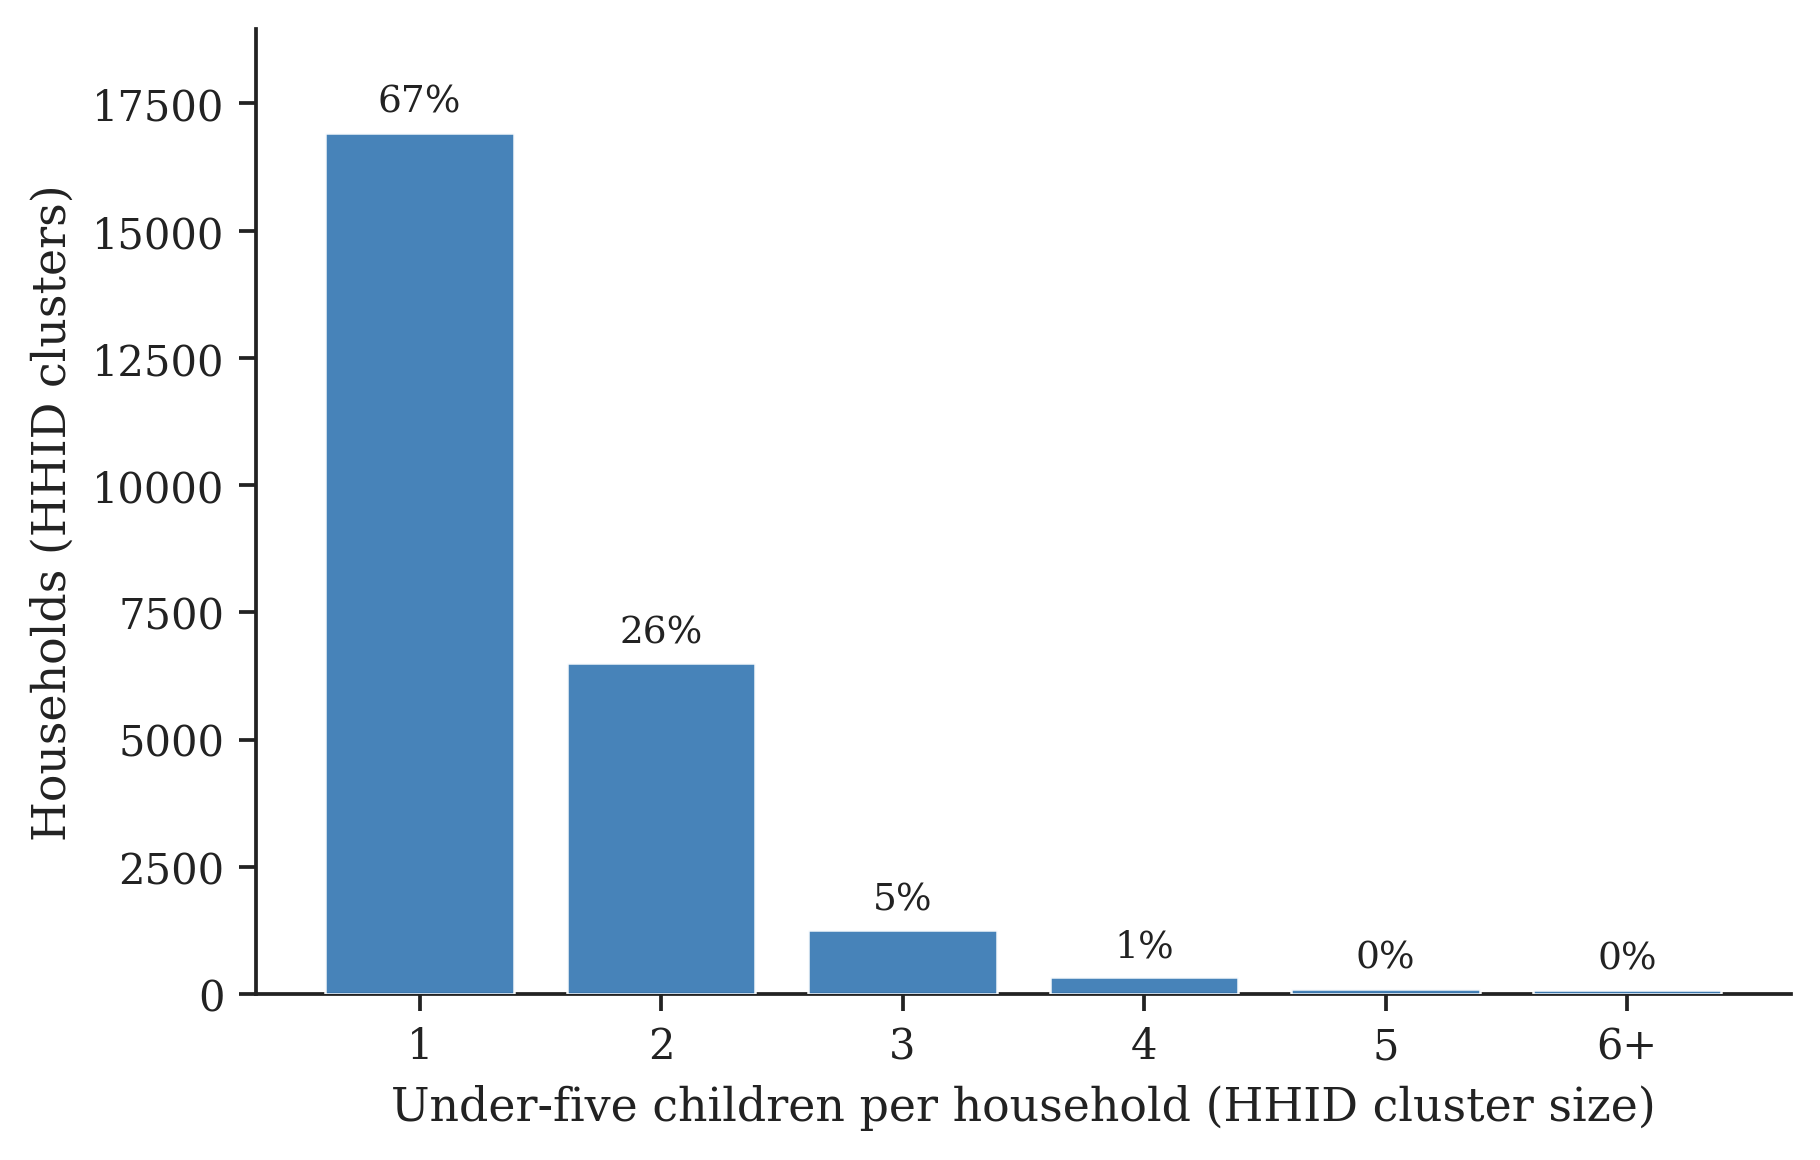
\includegraphics[width=0.62\linewidth]{children_distribution_U5.png}
{\footnotesize\begin{flushleft} \textit{Notes:} Each bar is the number of HHID clusters (households) contributing a given number of under-five children to the U5 estimation sample ($n=36{,}121$ children in $25{,}202$ households; bars are labelled with their share of households, and the ``6+'' bar pools larger households). The distribution is dominated by singletons: $67\%$ of households contribute exactly one under-five child and the mean cluster size is $1.43$. Because so few households contribute more than one child, the within-cluster correlation that clustering on HHID is meant to absorb has little to act on, and clustered and i.i.d.\ standard errors essentially coincide. This is what licenses reusing i.i.d.\ standard errors for APOS, which \texttt{doubleml} does not cluster natively (Section~\ref{sec:cluster}). \end{flushleft}}
\end{figure}


\clearpage
\section{Group heterogeneity tables}\label{app:gate_tables}\setcounter{figure}{0}\setcounter{table}{0}
The tables below report the full set of GATE results for every grouping variable used in the analysis. They keep the same APOS-to-GATE construction as the main text, but the layouts differ by group so the information stays readable: smaller groups appear as standard tables, while the country table uses a sideways layout because it is wide.

{\renewcommand\normalsize{\footnotesize}\normalsize\singlespacing
% Requires: \usepackage{booktabs, pdflscape, graphicx, adjustbox}
\begin{table}[p]
\centering
\caption{Group average treatment effects by source-water e.coli risk}
\label{tab:gate_risksource}
\small
\setlength{\tabcolsep}{4pt}
\begin{adjustbox}{max width=\linewidth, center}
\begin{tabular}{lccc}
\toprule
\multicolumn{4}{l}{\textbf{Panel A: Some Risk Home (E.coli 1--100 CFU) (HH)}} \\
Method vs. no treatment & No risk & Moderate & Very high \\
\midrule
Boil & -0.124*** (0.008) & -0.050*** (0.010) & 0.176*** (0.013) \\
Chlorine & -0.001 (0.016) & -0.043* (0.023) & 0.103*** (0.033) \\
Filter & 0.002 (0.009) & 0.053*** (0.013) & 0.133*** (0.019) \\
Other & -0.078*** (0.012) & -0.128*** (0.015) & 0.213*** (0.016) \\
\addlinespace
\multicolumn{4}{l}{\textbf{Panel B: Very High Risk Home (E.coli $\geq$ 101 CFU) (HH)}} \\
Method vs. no treatment & No risk & Moderate & Very high \\
\midrule
Boil & -0.027*** (0.004) & -0.105*** (0.008) & -0.272*** (0.015) \\
Chlorine & 0.059*** (0.012) & -0.064*** (0.020) & -0.142*** (0.034) \\
Filter & 0.055*** (0.006) & -0.051*** (0.011) & -0.148*** (0.020) \\
Other & -0.031*** (0.007) & -0.086*** (0.010) & -0.429*** (0.018) \\
\addlinespace
\multicolumn{4}{l}{\textbf{Panel C: Diarrhea (under-5) (U5)}} \\
Method vs. no treatment & No risk & Moderate & Very high \\
\midrule
Boil & -0.034*** (0.008) & -0.033*** (0.009) & -0.015 (0.011) \\
Chlorine & 0.023 (0.022) & -0.003 (0.019) & -0.027 (0.023) \\
Filter & 0.011 (0.012) & 0.045** (0.018) & -0.013 (0.021) \\
Other & -0.039** (0.015) & -0.064*** (0.012) & -0.008 (0.019) \\
\bottomrule
\end{tabular}
\end{adjustbox}
\par\vspace{3pt}
\begin{minipage}{\linewidth}\footnotesize \textit{Notes:} Cells report APOS-based group average treatment effects relative to no treatment. Standard errors are in parentheses. $^{***}p<0.01$, $^{**}p<0.05$, $^{*}p<0.10$.\end{minipage}
\end{table}

% Requires: \usepackage{booktabs, pdflscape, graphicx, adjustbox}
\begin{table}[p]
\centering
\caption{Group average treatment effects by household education}
\label{tab:gate_helevel}
\small
\setlength{\tabcolsep}{4pt}
\begin{adjustbox}{max width=\linewidth, center}
\begin{tabular}{lcccc}
\toprule
\multicolumn{5}{l}{\textbf{Panel A: Some Risk Home (E.coli 1--100 CFU) (HH)}} \\
Method vs. no treatment & None & Primary & Secondary & Missing \\
\midrule
Boil & 0.016* (0.009) & -0.025** (0.011) & -0.077*** (0.009) & 0.008 (0.037) \\
Chlorine & 0.056** (0.023) & -0.037 (0.024) & -0.009 (0.021) & 0.182*** (0.044) \\
Filter & 0.043*** (0.016) & 0.049*** (0.013) & 0.049*** (0.011) & 0.041 (0.031) \\
Other & -0.064*** (0.013) & -0.013 (0.015) & -0.032** (0.014) & -0.104* (0.053) \\
\addlinespace
\multicolumn{5}{l}{\textbf{Panel B: Very High Risk Home (E.coli $\geq$ 101 CFU) (HH)}} \\
Method vs. no treatment & None & Primary & Secondary & Missing \\
\midrule
Boil & -0.155*** (0.008) & -0.109*** (0.009) & -0.077*** (0.007) & -0.093*** (0.021) \\
Chlorine & -0.094*** (0.022) & -0.038* (0.022) & 0.003 (0.018) & 0.155*** (0.031) \\
Filter & -0.071*** (0.014) & -0.043*** (0.012) & 0.008 (0.009) & 0.036 (0.026) \\
Other & -0.166*** (0.012) & -0.172*** (0.012) & -0.093*** (0.009) & -0.048 (0.029) \\
\addlinespace
\multicolumn{5}{l}{\textbf{Panel C: Diarrhea (under-5) (U5)}} \\
Method vs. no treatment & None & Primary & Secondary & Missing \\
\midrule
Boil & -0.025*** (0.009) & -0.034*** (0.011) & -0.027*** (0.010) & -0.042 (0.027) \\
Chlorine & -0.037* (0.021) & -0.004 (0.022) & 0.031 (0.022) & 0.018 (0.013) \\
Filter & 0.032 (0.019) & -0.001 (0.017) & 0.019 (0.015) & 0.060 (0.058) \\
Other & -0.026* (0.016) & -0.047*** (0.015) & -0.046*** (0.015) & -0.041 (0.058) \\
\bottomrule
\end{tabular}
\end{adjustbox}
\par\vspace{3pt}
\begin{minipage}{\linewidth}\footnotesize \textit{Notes:} Cells report APOS-based group average treatment effects relative to no treatment. Standard errors are in parentheses. $^{***}p<0.01$, $^{**}p<0.05$, $^{*}p<0.10$.\end{minipage}
\end{table}

% Requires: \usepackage{booktabs, pdflscape, graphicx, adjustbox}
\begin{table}[p]
\centering
\caption{Group average treatment effects by wealth quintile}
\label{tab:gate_windex5}
\small
\setlength{\tabcolsep}{4pt}
\begin{adjustbox}{max width=\linewidth, center}
\begin{tabular}{lccccc}
\toprule
\multicolumn{6}{l}{\textbf{Panel A: Some Risk Home (E.coli 1--100 CFU) (HH)}} \\
Method vs. no treatment & Q1 & Q2 & Q3 & Q4 & Q5 \\
\midrule
Boil & -0.018 (0.013) & -0.031** (0.013) & -0.030** (0.013) & -0.059*** (0.012) & -0.048*** (0.012) \\
Chlorine & -0.021 (0.027) & 0.031 (0.026) & 0.024 (0.026) & 0.005 (0.030) & -0.010 (0.034) \\
Filter & 0.033* (0.017) & 0.083*** (0.016) & 0.022 (0.016) & 0.057*** (0.014) & 0.045*** (0.014) \\
Other & -0.075*** (0.014) & -0.025 (0.017) & -0.023 (0.019) & -0.047** (0.021) & 0.004 (0.026) \\
\addlinespace
\multicolumn{6}{l}{\textbf{Panel B: Very High Risk Home (E.coli $\geq$ 101 CFU) (HH)}} \\
Method vs. no treatment & Q1 & Q2 & Q3 & Q4 & Q5 \\
\midrule
Boil & -0.138*** (0.010) & -0.126*** (0.011) & -0.120*** (0.010) & -0.078*** (0.009) & -0.046*** (0.009) \\
Chlorine & -0.014 (0.026) & -0.072*** (0.024) & -0.047** (0.022) & -0.051** (0.024) & 0.057* (0.030) \\
Filter & -0.054*** (0.016) & -0.063*** (0.014) & -0.036*** (0.014) & -0.003 (0.012) & 0.051*** (0.012) \\
Other & -0.160*** (0.011) & -0.159*** (0.013) & -0.151*** (0.014) & -0.096*** (0.016) & -0.077*** (0.015) \\
\addlinespace
\multicolumn{6}{l}{\textbf{Panel C: Diarrhea (under-5) (U5)}} \\
Method vs. no treatment & Q1 & Q2 & Q3 & Q4 & Q5 \\
\midrule
Boil & -0.040*** (0.010) & -0.042*** (0.010) & -0.047*** (0.010) & 0.007 (0.017) & 0.001 (0.017) \\
Chlorine & -0.016 (0.022) & -0.018 (0.021) & 0.014 (0.025) & -0.010 (0.034) & 0.056 (0.042) \\
Filter & 0.001 (0.021) & 0.030 (0.022) & 0.020 (0.021) & 0.001 (0.018) & 0.052** (0.026) \\
Other & -0.059*** (0.014) & -0.019 (0.020) & -0.027 (0.020) & -0.010 (0.027) & -0.092*** (0.015) \\
\bottomrule
\end{tabular}
\end{adjustbox}
\par\vspace{3pt}
\begin{minipage}{\linewidth}\footnotesize \textit{Notes:} Cells report APOS-based group average treatment effects relative to no treatment. Standard errors are in parentheses. $^{***}p<0.01$, $^{**}p<0.05$, $^{*}p<0.10$.\end{minipage}
\end{table}

% Requires: \usepackage{booktabs, pdflscape, graphicx, adjustbox}
\begin{landscape}
\begin{table}[p]
\centering
\caption{Group average treatment effects by country}
\label{tab:gate_countrycat}
\scriptsize
\setlength{\tabcolsep}{4pt}
\begin{adjustbox}{max width=\linewidth, center}
\begin{tabular}{lccccccccccccccccccccccccc}
\toprule
\multicolumn{26}{l}{\textbf{Panel A: Some Risk Home (E.coli 1--100 CFU) (HH)}} \\
Method vs. no treatment & 2 & 3 & 4 & 5 & 8 & 9 & 10 & 11 & 12 & 13 & 14 & 15 & 16 & 18 & 19 & 20 & 21 & 22 & 23 & 24 & 25 & 26 & 28 & 31 & 32 \\
\midrule
Boil & -0.110*** (0.011) & 0.071*** (0.010) & -0.029 (0.020) & 0.170*** (0.012) & -0.251*** (0.012) & -0.026* (0.015) & -0.025 (0.026) & 0.079 (0.088) & -0.280*** (0.015) & -0.142*** (0.013) & 0.150*** (0.017) & -0.042 (0.027) & -0.070*** (0.017) & -0.051 (0.047) & -0.168*** (0.029) & 0.066** (0.032) & 0.079*** (0.017) & -0.062 (0.038) & -0.225*** (0.024) & 0.280*** (0.015) & -0.014 (0.042) & 0.201*** (0.022) & -0.021 (0.026) & -0.085 (0.052) & -0.043** (0.018) \\
Chlorine & -0.087*** (0.018) & 0.229*** (0.059) & -0.135 (0.126) & 0.063 (0.080) & -0.219*** (0.048) & -0.273*** (0.086) & 0.080 (0.126) & 0.117* (0.068) & -0.106** (0.051) & 0.050 (0.038) & 0.030 (0.084) & 0.153 (0.171) & 0.119 (0.088) & -0.067*** (0.012) & -0.018 (0.018) & 0.135*** (0.031) & -0.040 (0.071) & 0.216*** (0.016) & -0.156*** (0.017) & 0.166* (0.095) & -0.077** (0.036) & 0.054 (0.141) & 0.061 (0.066) & 0.021 (0.026) & -0.147*** (0.051) \\
Filter & -0.025 (0.021) & 0.165*** (0.022) & 0.008 (0.035) & 0.120*** (0.034) & 0.096*** (0.013) & 0.010 (0.021) & 0.061* (0.036) & 0.023 (0.085) & 0.102 (0.066) & -0.041* (0.025) & -0.098*** (0.022) & 0.006 (0.061) & 0.096** (0.039) & 0.033 (0.028) & 0.112*** (0.022) & 0.169*** (0.021) & 0.066** (0.028) & 0.030 (0.019) & -0.056 (0.052) & 0.019 (0.056) & 0.027 (0.085) & 0.105* (0.056) & 0.210*** (0.024) & -0.072** (0.036) & 0.112*** (0.016) \\
Other & -0.001 (0.035) & 0.086*** (0.026) & 0.009 (0.039) & 0.134*** (0.018) & -0.160*** (0.014) & -0.092*** (0.029) & -0.118*** (0.042) & 0.012 (0.084) & -0.245*** (0.020) & -0.030 (0.023) & -0.275*** (0.042) & -0.009 (0.044) & 0.049 (0.043) & 0.078* (0.047) & 0.039 (0.025) & 0.065*** (0.015) & -0.022 (0.024) & -0.157*** (0.044) & 0.086 (0.071) & -0.176*** (0.017) & 0.013 (0.057) & -0.181*** (0.049) & -0.109 (0.074) & -0.256*** (0.051) & 0.038** (0.017) \\
\addlinespace
\multicolumn{26}{l}{\textbf{Panel B: Very High Risk Home (E.coli $\geq$ 101 CFU) (HH)}} \\
Method vs. no treatment & 2 & 3 & 4 & 5 & 8 & 9 & 10 & 11 & 12 & 13 & 14 & 15 & 16 & 18 & 19 & 20 & 21 & 22 & 23 & 24 & 25 & 26 & 28 & 31 & 32 \\
\midrule
Boil & -0.099*** (0.009) & -0.282*** (0.009) & -0.160*** (0.018) & -0.217*** (0.012) & 0.020*** (0.008) & -0.075*** (0.012) & -0.104*** (0.018) & -0.078 (0.058) & -0.061*** (0.009) & -0.008 (0.011) & -0.081*** (0.009) & -0.071*** (0.020) & -0.029* (0.015) & -0.119*** (0.045) & -0.028 (0.019) & -0.135*** (0.031) & -0.112*** (0.016) & -0.143*** (0.017) & -0.051** (0.020) & -0.356*** (0.014) & -0.031 (0.023) & -0.259*** (0.020) & 0.030 (0.021) & -0.128*** (0.034) & -0.110*** (0.015) \\
Chlorine & -0.067*** (0.020) & -0.329*** (0.057) & -0.143 (0.113) & -0.047 (0.087) & 0.070*** (0.027) & 0.206*** (0.079) & -0.187* (0.102) & 0.093** (0.045) & 0.060* (0.034) & 0.024 (0.036) & -0.124* (0.065) & -0.257* (0.142) & -0.134* (0.078) & 0.117*** (0.010) & 0.043*** (0.011) & -0.231*** (0.028) & -0.119 (0.075) & 0.173*** (0.009) & 0.090*** (0.013) & -0.170* (0.090) & 0.163*** (0.018) & -0.000 (0.134) & 0.147*** (0.043) & 0.146*** (0.013) & -0.038 (0.035) \\
Filter & -0.061*** (0.020) & -0.227*** (0.019) & 0.033 (0.033) & -0.108*** (0.038) & -0.055*** (0.007) & 0.151*** (0.022) & -0.071** (0.031) & -0.038 (0.065) & 0.028 (0.056) & 0.118*** (0.023) & -0.030** (0.014) & -0.036 (0.049) & 0.010 (0.035) & -0.076*** (0.027) & 0.017 (0.012) & -0.134*** (0.021) & -0.015 (0.028) & 0.071*** (0.017) & 0.003 (0.048) & 0.004 (0.050) & 0.001 (0.067) & -0.177*** (0.056) & 0.026** (0.013) & 0.017 (0.028) & -0.005 (0.014) \\
Other & -0.032 (0.028) & -0.330*** (0.023) & -0.291*** (0.020) & -0.409*** (0.018) & 0.016** (0.007) & -0.109*** (0.021) & -0.116*** (0.036) & 0.067 (0.065) & -0.091*** (0.010) & -0.090*** (0.020) & -0.029 (0.029) & -0.132*** (0.022) & -0.102*** (0.026) & -0.166*** (0.039) & -0.045*** (0.012) & -0.465*** (0.009) & -0.206*** (0.027) & -0.047** (0.020) & -0.085* (0.046) & -0.111*** (0.019) & -0.043 (0.029) & 0.118* (0.066) & -0.016 (0.036) & -0.070** (0.031) & -0.257*** (0.013) \\
\addlinespace
\multicolumn{26}{l}{\textbf{Panel C: Diarrhea (under-5) (U5)}} \\
Method vs. no treatment & 2 & 3 & 4 & 5 & 8 & 9 & 10 & 11 & 12 & 13 & 14 & 15 & 16 & 18 & 19 & 20 & 21 & 22 & 23 & 24 & 25 & 26 & 28 & 31 & 32 \\
\midrule
Boil & 0.025 (0.015) & 0.019*** (0.006) & -0.128*** (0.013) & -0.124*** (0.014) & -0.088*** (0.008) & -0.103*** (0.016) & 0.005 (0.063) & -0.028 (0.044) & -0.171*** (0.010) & -0.032* (0.020) & 0.047*** (0.017) & -0.028 (0.060) & -0.022 (0.040) & 0.018 (0.026) & -0.070*** (0.019) & 0.012 (0.041) & -0.037 (0.036) & 0.001 (0.019) & 0.022 (0.044) & 0.190*** (0.021) & -0.048 (0.045) & -0.101*** (0.017) & -0.010 (0.075) & 0.019 (0.030) & -0.073*** (0.026) \\
Chlorine & 0.056** (0.027) & -0.016 (0.047) & 0.120 (0.110) & -0.116** (0.052) & 0.053 (0.055) & -0.093** (0.039) & 0.006 (0.093) & -0.051 (0.051) & -0.099** (0.049) & 0.037 (0.072) & -0.032 (0.032) & -0.125** (0.061) & -0.042 (0.032) & 0.057*** (0.006) & 0.050*** (0.014) & 0.008 (0.037) & 0.090 (0.107) & 0.060*** (0.009) & 0.029*** (0.009) & -0.086** (0.037) & 0.006 (0.019) & 0.048 (0.138) & -0.023 (0.049) & 0.045*** (0.014) & -0.030 (0.062) \\
Filter & 0.083** (0.040) & 0.009 (0.018) & -0.090** (0.043) & 0.007 (0.052) & 0.142*** (0.021) & 0.117 (0.077) & 0.209 (0.148) & -0.144*** (0.036) & 0.068 (0.048) & -0.037 (0.042) & 0.004 (0.010) & -0.006 (0.104) & -0.060 (0.050) & 0.081 (0.053) & -0.029 (0.022) & -0.030 (0.029) & -0.030 (0.055) & -0.016 (0.015) & -0.099** (0.041) & 0.011 (0.062) & -0.016 (0.072) & -0.080 (0.059) & 0.107 (0.086) & 0.081 (0.069) & 0.068 (0.046) \\
Other & -0.033 (0.041) & -0.003 (0.025) & -0.087* (0.045) & -0.078*** (0.029) & -0.077*** (0.008) & -0.133*** (0.015) & -0.093*** (0.017) & 0.180 (0.187) & -0.082*** (0.028) & -0.082*** (0.026) & 0.058 (0.051) & -0.097*** (0.018) & -0.023 (0.064) & 0.010 (0.051) & 0.007 (0.014) & -0.017 (0.022) & -0.121*** (0.039) & -0.043 (0.056) & -0.005 (0.074) & -0.035*** (0.011) & -0.095*** (0.016) & 0.054 (0.112) & 0.049 (0.143) & 0.023 (0.062) & -0.062*** (0.012) \\
\bottomrule
\end{tabular}
\end{adjustbox}
\par\vspace{3pt}
\begin{minipage}{\linewidth}\footnotesize \textit{Notes:} Cells report APOS-based group average treatment effects relative to no treatment. Standard errors are in parentheses. $^{***}p<0.01$, $^{**}p<0.05$, $^{*}p<0.10$.\end{minipage}
\end{table}
\end{landscape}

% Requires: \usepackage{booktabs, pdflscape, graphicx, adjustbox}
\begin{table}[p]
\centering
\caption{Group average treatment effects by toilet type}
\label{tab:gate_toilet}
\small
\setlength{\tabcolsep}{4pt}
\begin{adjustbox}{max width=\linewidth, center}
\begin{tabular}{lcccc}
\toprule
\multicolumn{5}{l}{\textbf{Panel A: Some Risk Home (E.coli 1--100 CFU) (HH)}} \\
Method vs. no treatment & Flush & Pit latrine & Open defecation & Missing \\
\midrule
Boil & -0.080*** (0.010) & -0.054*** (0.008) & 0.099*** (0.012) & 0.055 (0.054) \\
Chlorine & -0.008 (0.019) & -0.012 (0.022) & 0.070** (0.027) & 0.046 (0.061) \\
Filter & 0.035*** (0.013) & 0.024** (0.011) & 0.120*** (0.016) & 0.124*** (0.040) \\
Other & -0.034** (0.017) & -0.062*** (0.010) & -0.002 (0.013) & 0.094*** (0.022) \\
\addlinespace
\multicolumn{5}{l}{\textbf{Panel B: Very High Risk Home (E.coli $\geq$ 101 CFU) (HH)}} \\
Method vs. no treatment & Flush & Pit latrine & Open defecation & Missing \\
\midrule
Boil & -0.051*** (0.008) & -0.114*** (0.006) & -0.212*** (0.011) & -0.116** (0.054) \\
Chlorine & 0.027* (0.015) & -0.037* (0.020) & -0.114*** (0.027) & -0.154*** (0.058) \\
Filter & 0.023** (0.010) & -0.020** (0.010) & -0.144*** (0.015) & -0.076** (0.037) \\
Other & -0.060*** (0.011) & -0.128*** (0.008) & -0.275*** (0.012) & -0.435*** (0.017) \\
\addlinespace
\multicolumn{5}{l}{\textbf{Panel C: Diarrhea (under-5) (U5)}} \\
Method vs. no treatment & Flush & Pit latrine & Open defecation & Missing \\
\midrule
Boil & -0.010 (0.012) & -0.036*** (0.007) & -0.033*** (0.010) & -0.045 (0.055) \\
Chlorine & 0.013 (0.016) & 0.010 (0.021) & -0.029 (0.024) & -0.040* (0.023) \\
Filter & 0.038* (0.020) & 0.016 (0.013) & 0.006 (0.022) & -0.050** (0.021) \\
Other & -0.039** (0.019) & -0.029** (0.013) & -0.062*** (0.013) & -0.047*** (0.013) \\
\bottomrule
\end{tabular}
\end{adjustbox}
\par\vspace{3pt}
\begin{minipage}{\linewidth}\footnotesize \textit{Notes:} Cells report APOS-based group average treatment effects relative to no treatment. Standard errors are in parentheses. $^{***}p<0.01$, $^{**}p<0.05$, $^{*}p<0.10$.\end{minipage}
\end{table}

% Requires: \usepackage{booktabs, pdflscape, graphicx, adjustbox}
\begin{table}[p]
\centering
\caption{Group average treatment effects by water source type}
\label{tab:gate_ws1g}
\small
\setlength{\tabcolsep}{4pt}
\begin{adjustbox}{max width=\linewidth, center}
\begin{tabular}{lccccccc}
\toprule
\multicolumn{8}{l}{\textbf{Panel A: Some Risk Home (E.coli 1--100 CFU) (HH)}} \\
Method vs. no treatment & Piped & Tube/well/borehole & Protected well/spring & Unprotected well/spring & Surface/rain & Packaged/bottled & Other \\
\midrule
Boil & -0.106*** (0.011) & -0.050*** (0.009) & 0.015 (0.034) & 0.070*** (0.015) & 0.052** (0.021) & -0.036*** (0.011) & 0.003 (0.051) \\
Chlorine & -0.012 (0.026) & -0.017 (0.020) & -0.025 (0.056) & 0.066** (0.033) & 0.034 (0.052) & 0.022 (0.024) & 0.032 (0.113) \\
Filter & 0.047*** (0.015) & 0.013 (0.011) & 0.037 (0.027) & 0.101*** (0.019) & 0.088** (0.038) & 0.040*** (0.012) & 0.084* (0.046) \\
Other & -0.031* (0.018) & -0.069*** (0.017) & 0.040 (0.031) & -0.050*** (0.014) & 0.024 (0.027) & -0.053*** (0.017) & -0.063 (0.064) \\
\addlinespace
\multicolumn{8}{l}{\textbf{Panel B: Very High Risk Home (E.coli $\geq$ 101 CFU) (HH)}} \\
Method vs. no treatment & Piped & Tube/well/borehole & Protected well/spring & Unprotected well/spring & Surface/rain & Packaged/bottled & Other \\
\midrule
Boil & -0.051*** (0.009) & -0.118*** (0.007) & -0.202*** (0.027) & -0.200*** (0.014) & -0.167*** (0.018) & -0.030*** (0.007) & -0.122*** (0.022) \\
Chlorine & -0.023 (0.022) & -0.078*** (0.019) & -0.082 (0.053) & -0.096*** (0.033) & -0.055 (0.049) & 0.136*** (0.020) & 0.127 (0.089) \\
Filter & 0.007 (0.013) & -0.052*** (0.010) & -0.069*** (0.025) & -0.137*** (0.018) & -0.104*** (0.033) & 0.106*** (0.008) & 0.047 (0.043) \\
Other & -0.089*** (0.011) & -0.099*** (0.014) & -0.259*** (0.020) & -0.242*** (0.013) & -0.273*** (0.022) & -0.049*** (0.010) & -0.064 (0.040) \\
\addlinespace
\multicolumn{8}{l}{\textbf{Panel C: Diarrhea (under-5) (U5)}} \\
Method vs. no treatment & Piped & Tube/well/borehole & Protected well/spring & Unprotected well/spring & Surface/rain & Packaged/bottled & Other \\
\midrule
Boil & -0.040*** (0.012) & -0.034*** (0.008) & -0.003 (0.017) & -0.041*** (0.011) & -0.002 (0.024) & 0.005 (0.022) & -0.086*** (0.024) \\
Chlorine & -0.001 (0.025) & 0.028 (0.029) & 0.019 (0.041) & -0.004 (0.027) & -0.077** (0.031) & -0.021* (0.011) & 0.067 (0.066) \\
Filter & 0.022 (0.021) & 0.020 (0.018) & 0.025 (0.030) & 0.036 (0.023) & -0.011 (0.039) & 0.007 (0.008) & -0.117* (0.068) \\
Other & -0.034* (0.020) & -0.034* (0.018) & -0.024 (0.031) & -0.037** (0.015) & -0.041 (0.029) & -0.086*** (0.008) & -0.137*** (0.026) \\
\bottomrule
\end{tabular}
\end{adjustbox}
\par\vspace{3pt}
\begin{minipage}{\linewidth}\footnotesize \textit{Notes:} Cells report APOS-based group average treatment effects relative to no treatment. Standard errors are in parentheses. $^{***}p<0.01$, $^{**}p<0.05$, $^{*}p<0.10$.\end{minipage}
\end{table}

% Requires: \usepackage{booktabs, pdflscape, graphicx, adjustbox}
\begin{table}[p]
\centering
\caption{Group average treatment effects by number of children}
\label{tab:gate_numchildrenbin}
\small
\setlength{\tabcolsep}{4pt}
\begin{adjustbox}{max width=\linewidth, center}
\begin{tabular}{lccc}
\toprule
\multicolumn{4}{l}{\textbf{Panel A: Some Risk Home (E.coli 1--100 CFU) (HH)}} \\
Method vs. no treatment & 0 & 1 & 2 \\
\midrule
Boil & -0.036*** (0.006) & -0.060 (0.040) & -0.002 (0.034) \\
Chlorine & 0.004 (0.013) & 0.105 (0.119) & -0.028 (0.112) \\
Filter & 0.049*** (0.007) & -0.002 (0.078) & 0.032 (0.074) \\
Other & -0.039*** (0.009) & 0.038 (0.058) & -0.024 (0.047) \\
\addlinespace
\multicolumn{4}{l}{\textbf{Panel B: Very High Risk Home (E.coli $\geq$ 101 CFU) (HH)}} \\
Method vs. no treatment & 0 & 1 & 2 \\
\midrule
Boil & -0.109*** (0.005) & -0.049* (0.026) & -0.050*** (0.019) \\
Chlorine & -0.027** (0.011) & -0.173* (0.099) & 0.077 (0.089) \\
Filter & -0.026*** (0.006) & 0.019 (0.062) & -0.043 (0.058) \\
Other & -0.136*** (0.006) & -0.097*** (0.029) & -0.074*** (0.024) \\
\addlinespace
\multicolumn{4}{l}{\textbf{Panel C: Diarrhea (under-5) (U5)}} \\
Method vs. no treatment & 0 & 1 & 2 \\
\midrule
Boil & -0.028*** (0.006) & -0.026 (0.048) & -0.080*** (0.026) \\
Chlorine & 0.002 (0.013) & -0.021 (0.031) & -0.108** (0.049) \\
Filter & 0.019* (0.010) & 0.063 (0.078) & -0.220*** (0.056) \\
Other & -0.038*** (0.009) & -0.121*** (0.015) & -0.026* (0.016) \\
\bottomrule
\end{tabular}
\end{adjustbox}
\par\vspace{3pt}
\begin{minipage}{\linewidth}\footnotesize \textit{Notes:} Cells report APOS-based group average treatment effects relative to no treatment. Standard errors are in parentheses. $^{***}p<0.01$, $^{**}p<0.05$, $^{*}p<0.10$.\end{minipage}
\end{table}

% Requires: \usepackage{booktabs, pdflscape, graphicx, adjustbox}
\begin{table}[p]
\centering
\caption{Group average treatment effects by child age}
\label{tab:gate_childage}
\small
\setlength{\tabcolsep}{4pt}
\begin{adjustbox}{max width=\linewidth, center}
\begin{tabular}{lccccc}
\toprule
\multicolumn{6}{l}{\textbf{Panel A: Diarrhea (under-5) (U5)}} \\
Method vs. no treatment & 0 & 1 & 2 & 3 & 4 \\
\midrule
Boil & -0.026* (0.015) & -0.064*** (0.015) & -0.036*** (0.013) & -0.018** (0.009) & -0.002 (0.010) \\
Chlorine & 0.039 (0.036) & -0.055** (0.028) & -0.018 (0.022) & 0.005 (0.023) & 0.025 (0.025) \\
Filter & 0.018 (0.023) & -0.011 (0.023) & 0.018 (0.023) & 0.028 (0.021) & 0.036* (0.020) \\
Other & -0.034 (0.024) & -0.063** (0.025) & -0.086*** (0.013) & -0.027 (0.017) & 0.006 (0.017) \\
\bottomrule
\end{tabular}
\end{adjustbox}
\par\vspace{3pt}
\begin{minipage}{\linewidth}\footnotesize \textit{Notes:} Cells report APOS-based group average treatment effects relative to no treatment. Standard errors are in parentheses. $^{***}p<0.01$, $^{**}p<0.05$, $^{*}p<0.10$.\end{minipage}
\end{table}
}


\clearpage
\section{Overlap diagnostics on the restricted sample (robust specification)}\label{app:overlap_rob1}\setcounter{figure}{0}\setcounter{table}{0}
As a robustness check we drop the country cells in which a method is used by fewer than $5\%$ (or fewer than ten) of households --- the cells with the weakest within-country support --- and re-estimate on the restricted sample. The overlap diagnostics on that sample, for both estimators and all three outcomes, are shown below. They are visually indistinguishable from the full-sample diagnostics in the main text, and the resulting estimates change negligibly.

\begin{figure}[htbp]\centering
\caption{Robust specification --- overlap diagnostics (IRM), Some Risk Home E.\,coli}\label{fig:overlap_rob1_irm}
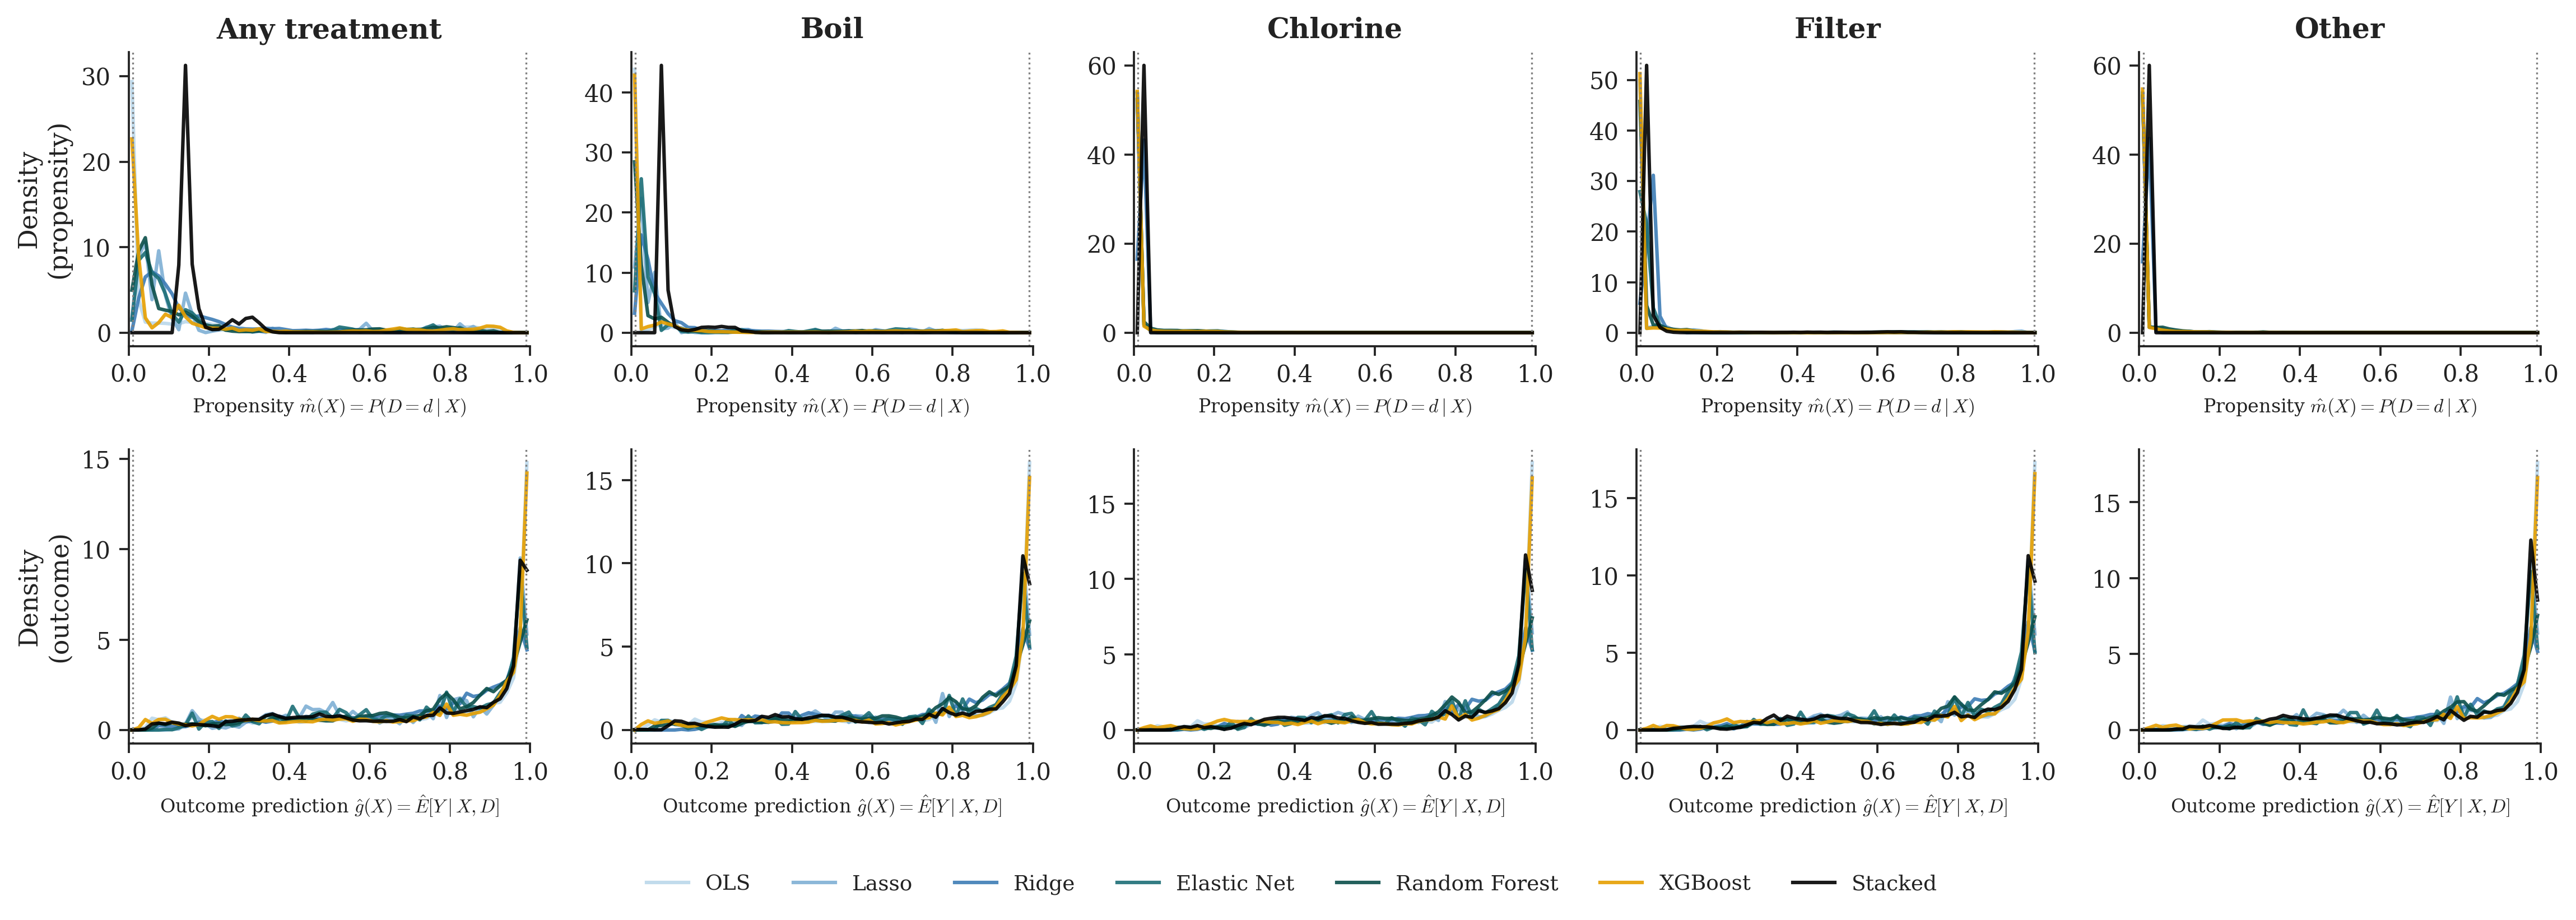
\includegraphics[width=\linewidth]{overlap_rob1_HH_SomeRiskHome.png}
\end{figure}

\begin{figure}[htbp]\centering
\caption{Robust specification --- overlap diagnostics (IRM), Very High Risk Home E.\,coli}\label{fig:overlap_rob1_irm_vh}
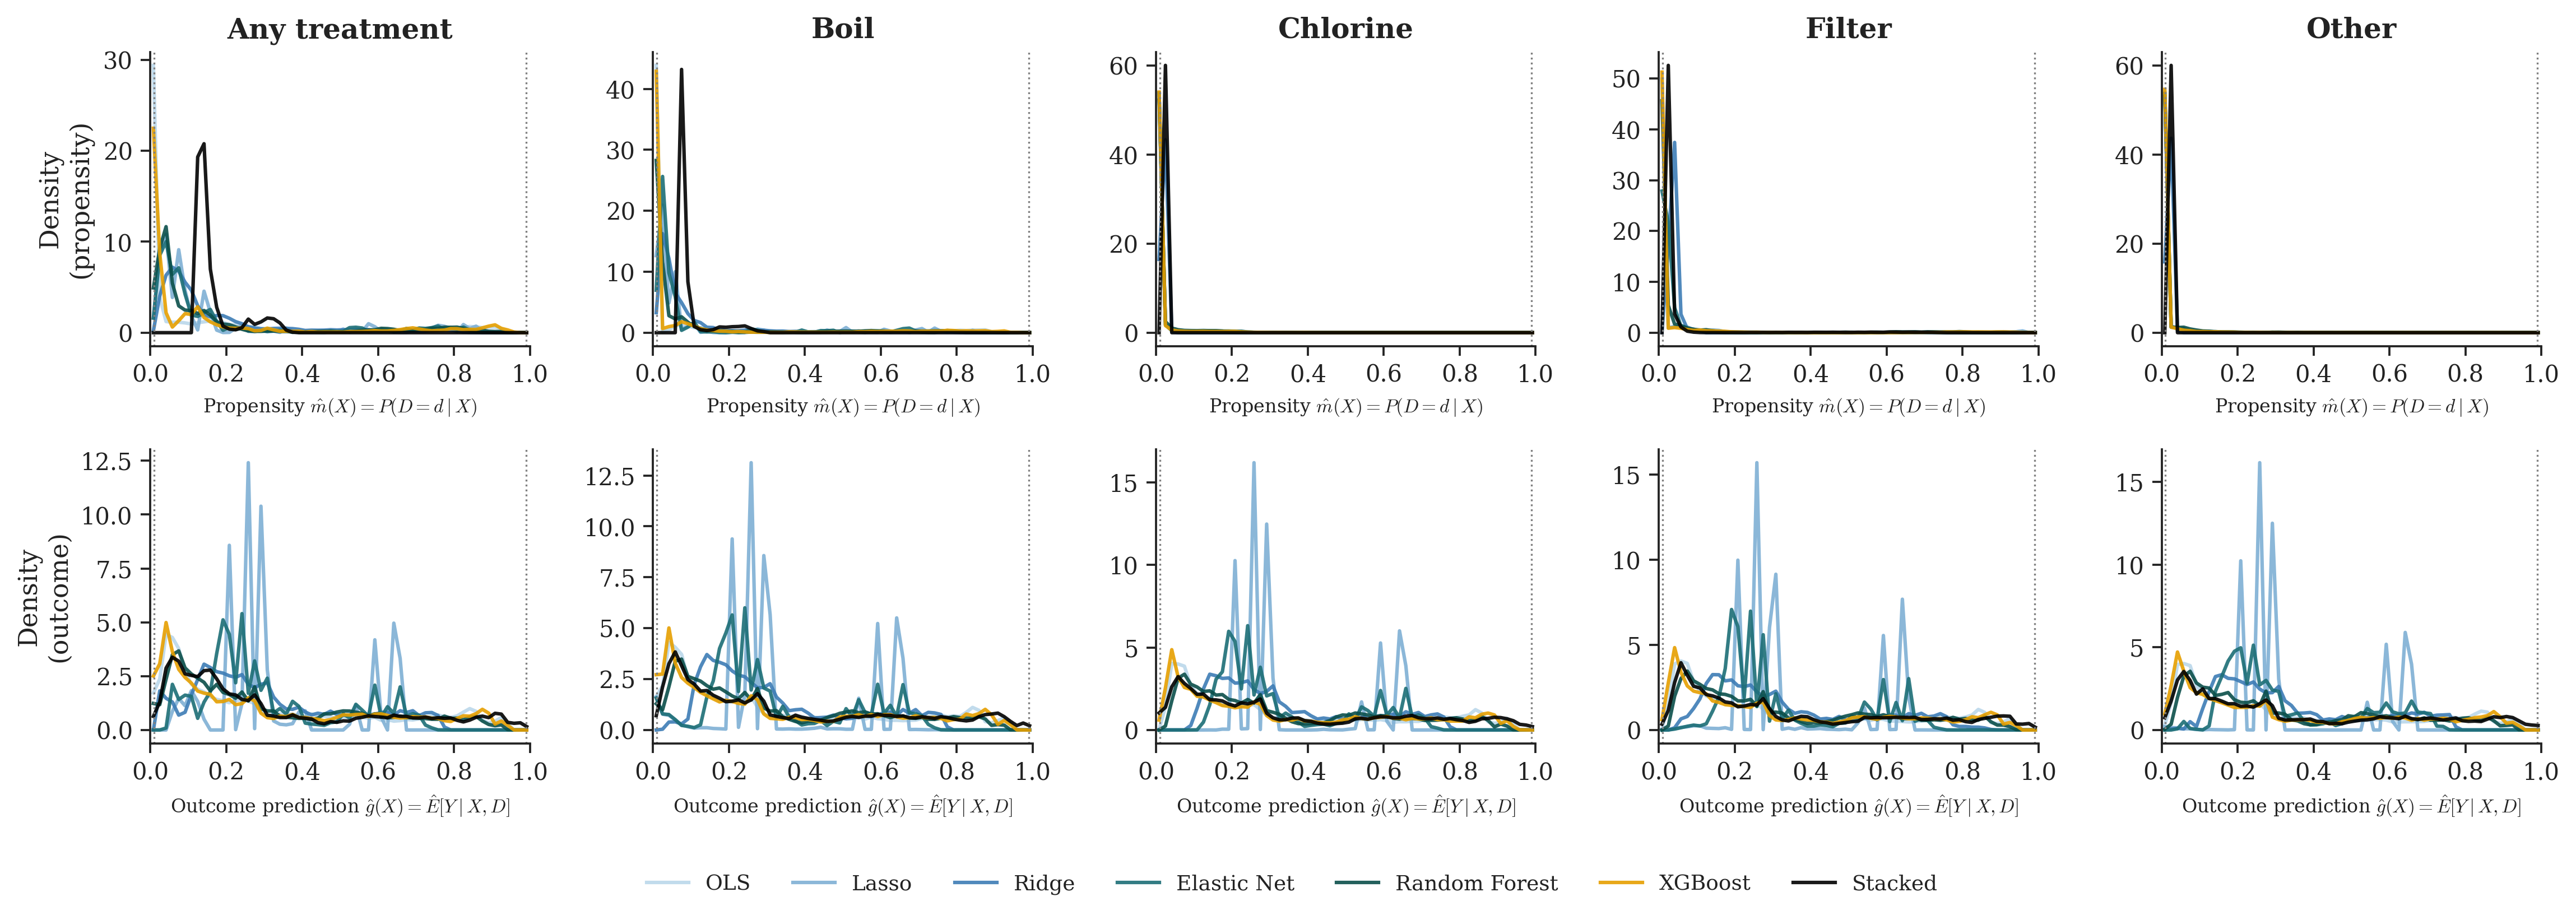
\includegraphics[width=\linewidth]{overlap_rob1_HH_VeryHighRiskHome.png}
\end{figure}

\begin{figure}[htbp]\centering
\caption{Robust specification --- overlap diagnostics (IRM), under-five diarrhea}\label{fig:overlap_rob1_irm_u5}
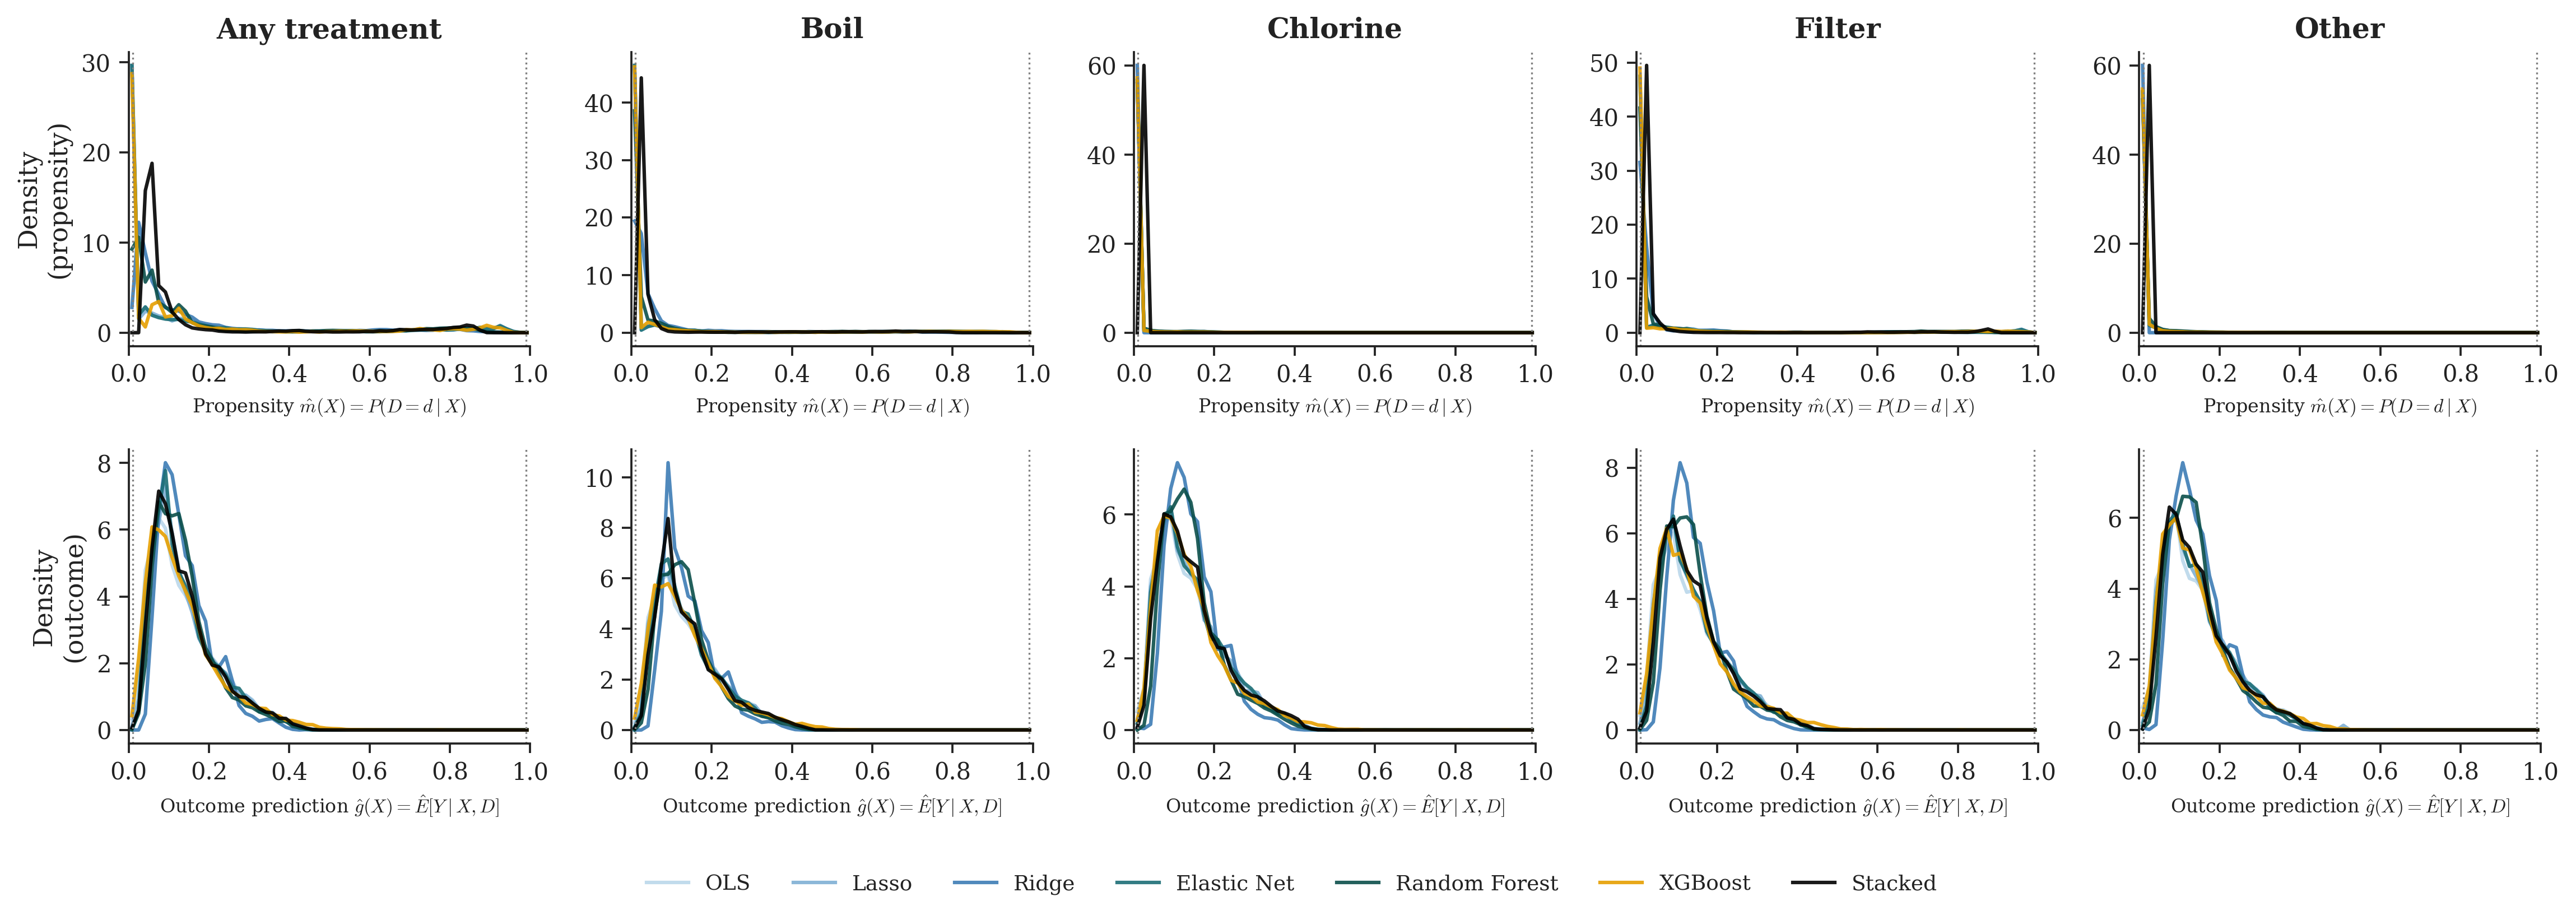
\includegraphics[width=\linewidth]{overlap_rob1_U5_diarrhea.png}
\end{figure}

\begin{figure}[htbp]\centering
\caption{Robust specification --- overlap diagnostics (APOS), Some Risk Home E.\,coli}\label{fig:overlap_rob1_apos}
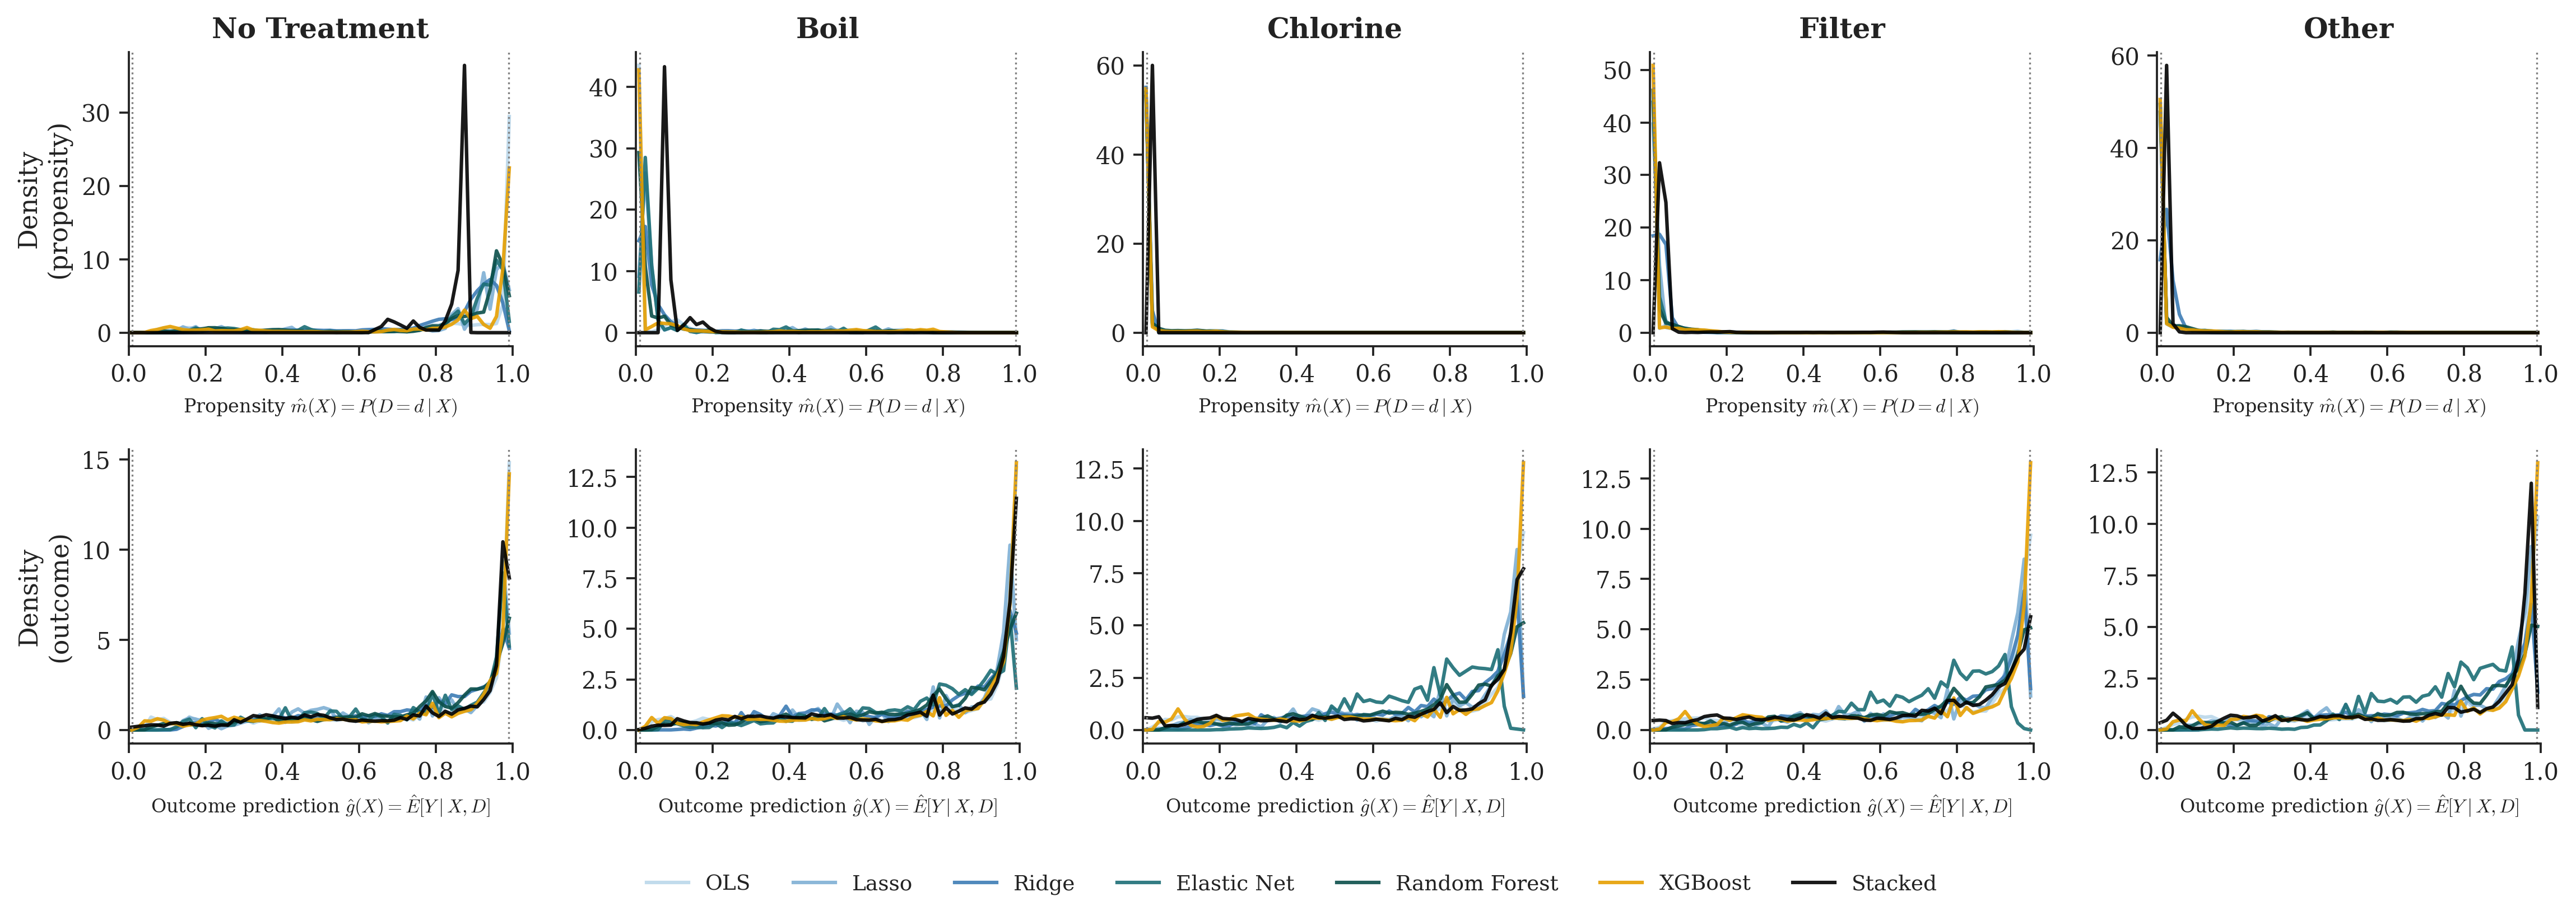
\includegraphics[width=\linewidth]{overlap_rob1_apos_HH_SomeRiskHome.png}
\end{figure}

\begin{figure}[htbp]\centering
\caption{Robust specification --- overlap diagnostics (APOS), Very High Risk Home E.\,coli}\label{fig:overlap_rob1_apos_vh}
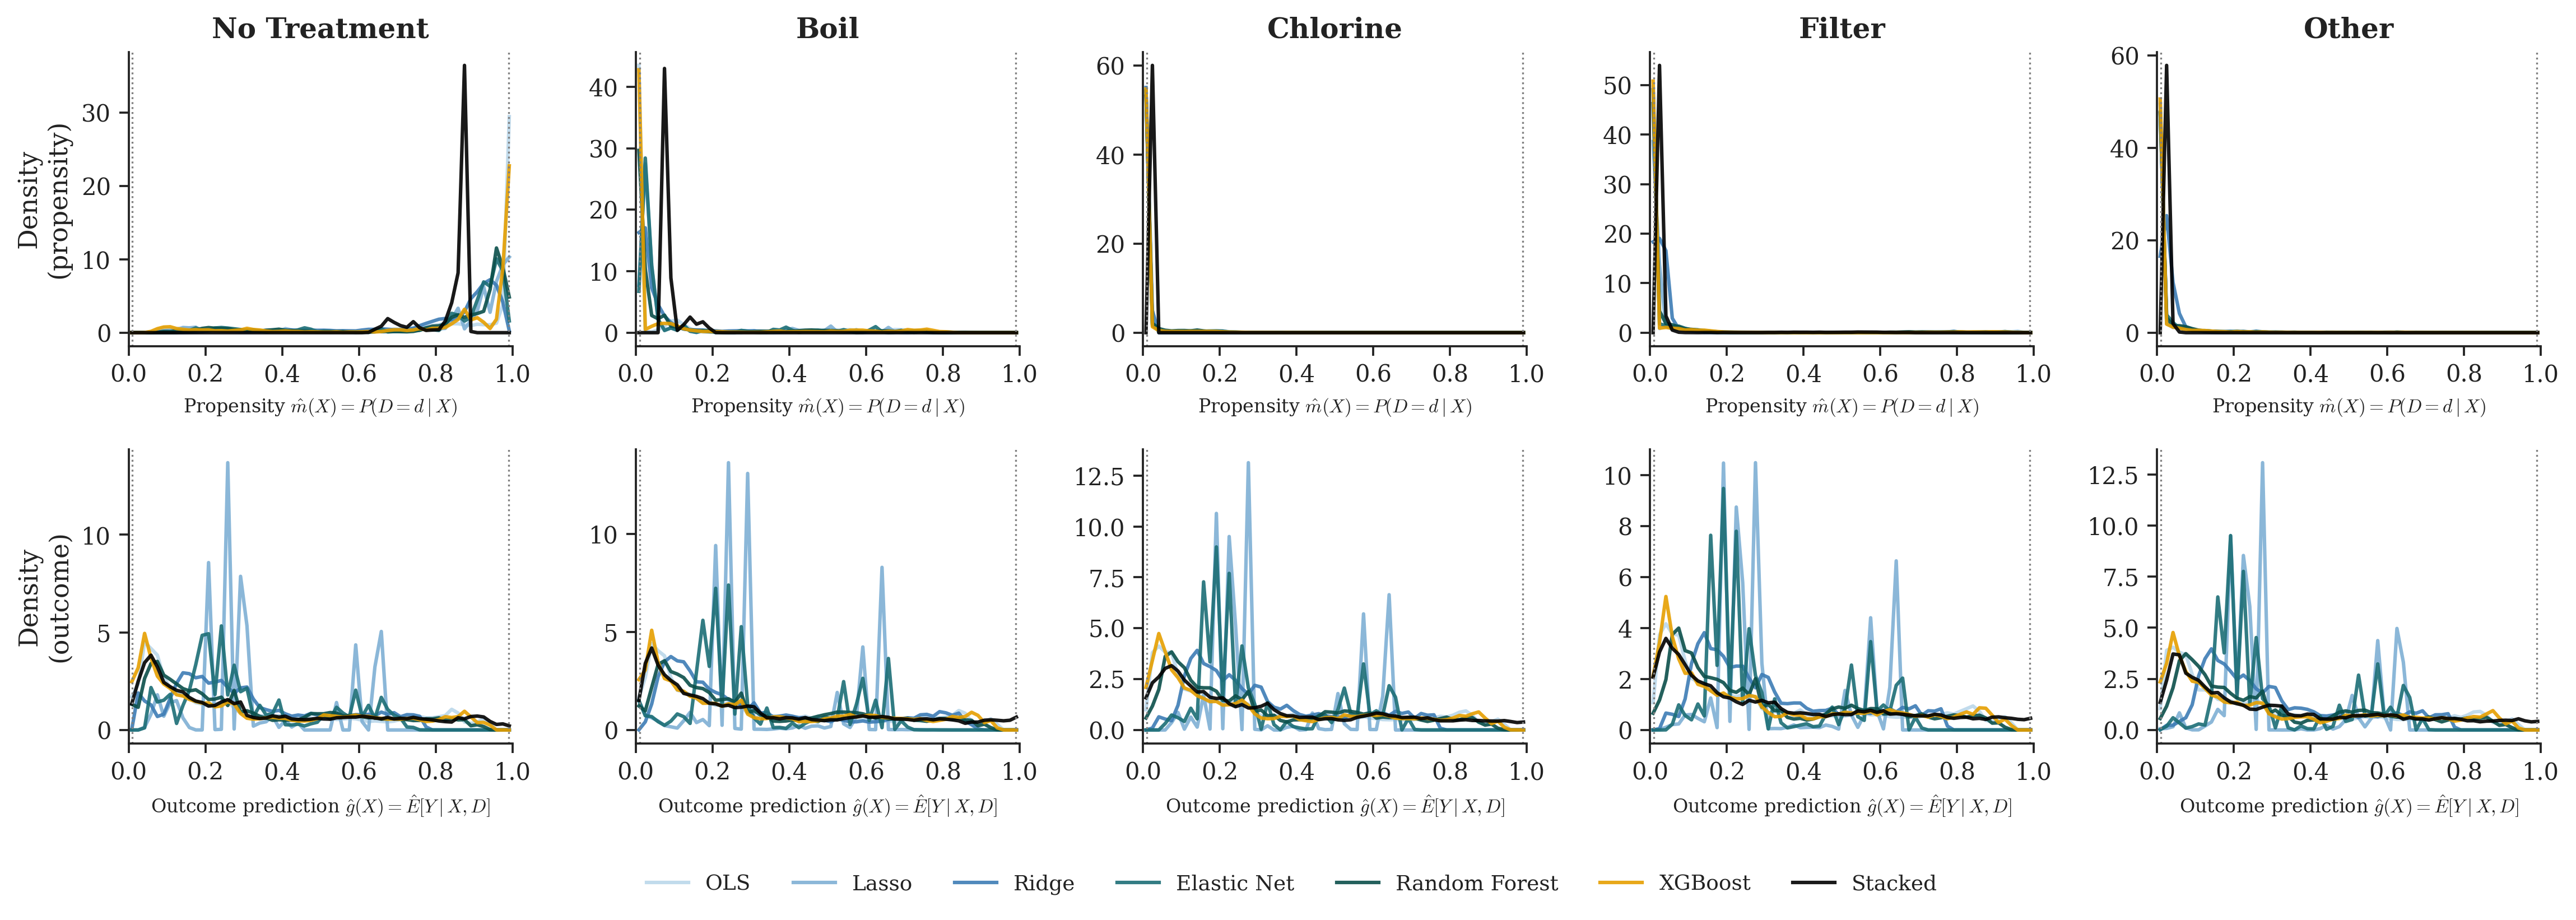
\includegraphics[width=\linewidth]{overlap_rob1_apos_HH_VeryHighRiskHome.png}
\end{figure}

\begin{figure}[htbp]\centering
\caption{Robust specification --- overlap diagnostics (APOS), under-five diarrhea}\label{fig:overlap_rob1_apos_u5}
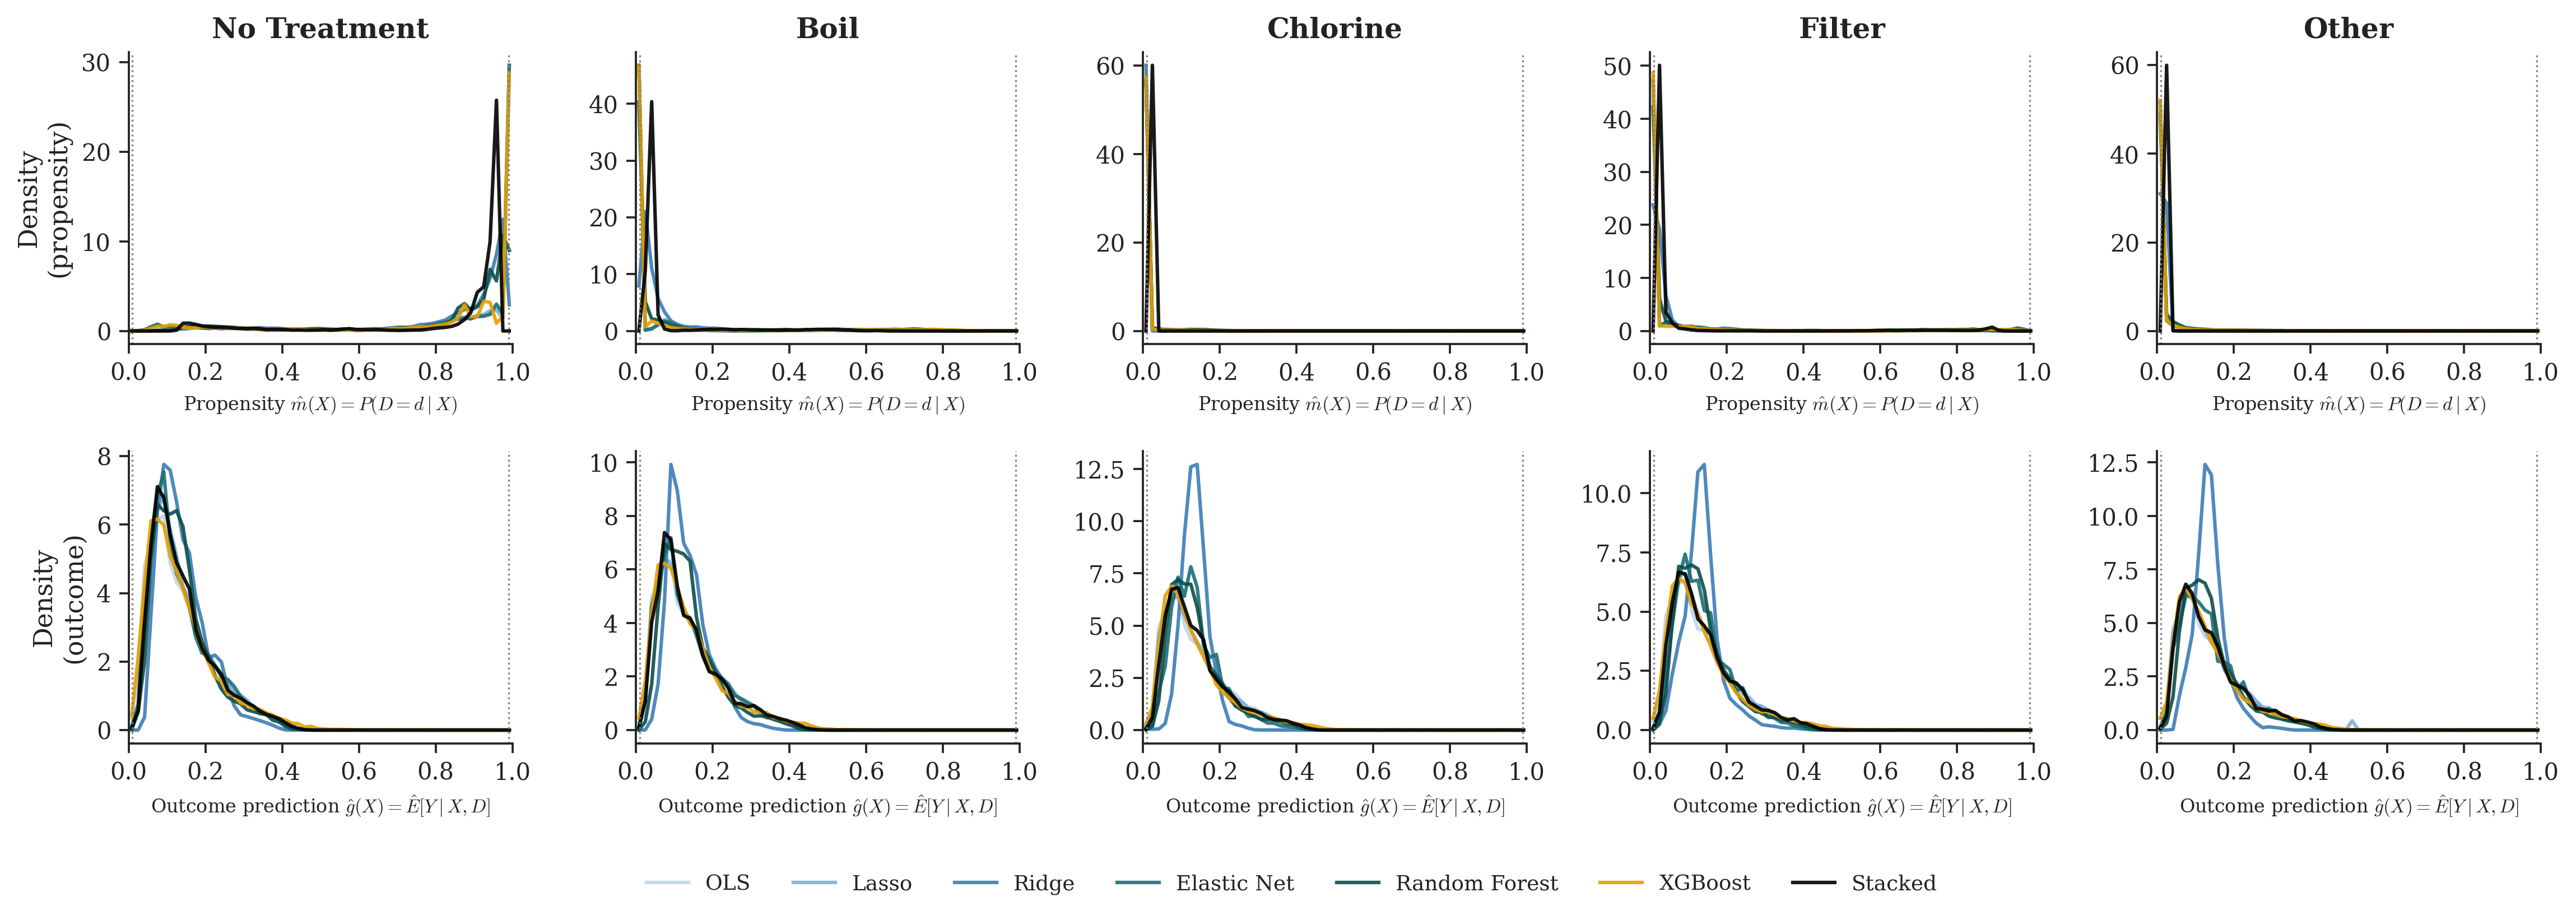
\includegraphics[width=\linewidth]{overlap_rob1_apos_U5_diarrhea.png}
\end{figure}


\clearpage\section{Robust specification: full estimation tables}\label{app:robust_tables}\setcounter{figure}{0}\setcounter{table}{0}
These tables re-estimate the headline specifications on the overlap-restricted sample, which drops the country cells where a method has weak within-country support (Appendix~\ref{app:overlap_rob1}). They are the robust-specification counterparts referenced from the main text: the IRM and APOS coefficient estimates (Tables~\ref{tab:irm-rob1} and~\ref{tab:apos-rob1}) and the confounder-benchmark sensitivity (Tables~\ref{tab:sensitivity-benchmark-irm-rob1} and~\ref{tab:sensitivity-benchmark-rob1}). Across all four, the qualitative conclusions of the main text are preserved.

% Requires: \usepackage{booktabs, pdflscape, graphicx}
\begin{landscape}
\begin{table}[htbp]
\centering
\caption{DDML IRM Estimates: Robust Specification (Overlap-Restricted Sample)}
\label{tab:irm-rob1}
\footnotesize
\setlength{\tabcolsep}{3pt}
\resizebox{\linewidth}{!}{%
\begin{tabular}{l|ccccccc|ccccccc|ccccccc}
\toprule
 & \multicolumn{7}{c|}{Some Risk Home (E.coli 1--100 CFU)} & \multicolumn{7}{c|}{Very High Risk Home (E.coli $\geq$ 101 CFU)} & \multicolumn{7}{c}{Diarrhea (under-5)} \\
\cmidrule(lr){2-8} \cmidrule(lr){9-15} \cmidrule(lr){16-22}
 & OLS & Lasso & Ridge & Elastic Net & Random Forest & XGBoost & Stacked & OLS & Lasso & Ridge & Elastic Net & Random Forest & XGBoost & Stacked & OLS & Lasso & Ridge & Elastic Net & Random Forest & XGBoost & Stacked \\
\midrule
\multicolumn{22}{l}{\textit{Panel A: Any treatment}} \\
Any treatment & -0.103*** & -0.094*** & -0.152*** & -0.124*** & -0.075*** & -0.087*** & -0.098*** & -0.100*** & -0.121*** & -0.119*** & -0.119*** & -0.106*** & -0.122*** & -0.109*** & -0.064*** & -0.044*** & -0.060*** & -0.043*** & -0.046*** & -0.048*** & -0.045*** \\
 & (0.006) & (0.006) & (0.004) & (0.005) & (0.003) & (0.004) & (0.003) & (0.005) & (0.006) & (0.004) & (0.005) & (0.004) & (0.004) & (0.003) & (0.005) & (0.005) & (0.005) & (0.005) & (0.004) & (0.004) & (0.005) \\
\quad $w_g$ & 0.10 & 0.11 & 0.03 & 0.17 & 0.24 & 0.35 &  & 0.20 & 0.09 & 0.11 & 0.09 & 0.27 & 0.24 &  & 0.19 & 0.16 & 0.18 & 0.15 & 0.14 & 0.18 &  \\
\quad $w_m$ & 0.21 & 0.19 & 0.17 & 0.17 & 0.15 & 0.11 &  & 0.20 & 0.19 & 0.17 & 0.17 & 0.15 & 0.11 &  & 0.20 & 0.16 & 0.09 & 0.15 & 0.17 & 0.22 &  \\
\quad RV & 0.03 & 0.05 & 0.09 & 0.07 & 0.03 & 0.03 & 0.09 & 0.03 & 0.04 & 0.07 & 0.06 & 0.04 & 0.03 & 0.08 & 0.02 & 0.01 & 0.03 & 0.01 & 0.02 & 0.01 & 0.02 \\
\quad RV$_\alpha$ & 0.03 & 0.05 & 0.09 & 0.06 & 0.03 & 0.03 & 0.08 & 0.02 & 0.04 & 0.06 & 0.05 & 0.04 & 0.03 & 0.08 & 0.02 & 0.01 & 0.02 & 0.01 & 0.02 & 0.01 & 0.02 \\
\quad $N$ & \multicolumn{7}{c|}{56,723} & \multicolumn{7}{c|}{56,723} & \multicolumn{7}{c}{34,639} \\
\midrule
\multicolumn{22}{l}{\textit{Panel B: Specific treatments (vs.\ no treatment)}} \\
Boil & -0.200*** & -0.214*** & -0.253*** & -0.243*** & -0.153*** & -0.185*** & -0.181*** & -0.136*** & -0.175*** & -0.157*** & -0.174*** & -0.149*** & -0.160*** & -0.128*** & -0.047*** & -0.048*** & -0.037*** & -0.049*** & -0.053*** & -0.054*** & -0.047*** \\
 & (0.005) & (0.005) & (0.003) & (0.005) & (0.003) & (0.003) & (0.004) & (0.004) & (0.004) & (0.003) & (0.004) & (0.003) & (0.003) & (0.004) & (0.004) & (0.004) & (0.005) & (0.004) & (0.003) & (0.004) & (0.005) \\
\quad $w_g$ & 0.09 & 0.10 & 0.06 & 0.11 & 0.30 & 0.34 &  & 0.22 & 0.12 & 0.22 & 0.10 & 0.20 & 0.14 &  & 0.21 & 0.12 & 0.21 & 0.11 & 0.20 & 0.16 &  \\
\quad $w_m$ & 0.19 & 0.18 & 0.09 & 0.19 & 0.15 & 0.19 &  & 0.19 & 0.18 & 0.09 & 0.19 & 0.14 & 0.19 &  & 0.21 & 0.18 & 0.06 & 0.18 & 0.16 & 0.20 &  \\
\quad RV & 0.05 & 0.07 & 0.10 & 0.09 & 0.04 & 0.05 & 0.12 & 0.03 & 0.06 & 0.06 & 0.06 & 0.04 & 0.03 & 0.07 & 0.01 & 0.01 & 0.01 & 0.01 & 0.01 & 0.01 & 0.02 \\
\quad RV$_\alpha$ & 0.05 & 0.07 & 0.10 & 0.08 & 0.04 & 0.04 & 0.11 & 0.03 & 0.05 & 0.06 & 0.05 & 0.04 & 0.03 & 0.07 & 0.01 & 0.01 & 0.01 & 0.01 & 0.01 & 0.01 & 0.01 \\
\quad $N$ & \multicolumn{7}{c|}{52,334} & \multicolumn{7}{c|}{52,334} & \multicolumn{7}{c}{31,552} \\
\midrule
Chlorine & -0.011* & -0.007 & -0.007 & -0.005 & -0.008 & 0.018*** & 0.006 & -0.037*** & -0.066*** & -0.075*** & -0.068*** & -0.067*** & -0.048*** & -0.035*** & 0.013*** & -0.020*** & -0.074*** & -0.010** & -0.020*** & -0.026*** & -0.028*** \\
 & (0.006) & (0.005) & (0.009) & (0.005) & (0.005) & (0.007) & (0.009) & (0.006) & (0.005) & (0.011) & (0.005) & (0.005) & (0.007) & (0.011) & (0.005) & (0.004) & (0.020) & (0.004) & (0.006) & (0.008) & (0.011) \\
\quad $w_g$ & 0.13 & 0.13 & 0.09 & 0.12 & 0.19 & 0.34 &  & 0.15 & 0.19 & 0.16 & 0.18 & 0.19 & 0.13 &  & 0.27 & 0.15 & 0.20 & 0.14 & 0.09 & 0.15 &  \\
\quad $w_m$ & 0.24 & 0.23 & 0.01 & 0.08 & 0.23 & 0.22 &  & 0.24 & 0.23 & 0.01 & 0.08 & 0.23 & 0.22 &  & 0.20 & 0.18 & 0.07 & 0.17 & 0.13 & 0.25 &  \\
\quad RV & 0.00 & 0.00 & 0.00 & 0.00 & 0.00 & 0.00 & 0.00 & 0.01 & 0.01 & 0.02 & 0.01 & 0.01 & 0.01 & 0.01 & 0.00 & 0.00 & 0.02 & 0.00 & 0.00 & 0.01 & 0.01 \\
\quad RV$_\alpha$ & 0.00 & 0.00 & 0.00 & 0.00 & 0.00 & 0.00 & 0.00 & 0.01 & 0.01 & 0.02 & 0.01 & 0.01 & 0.01 & 0.01 & 0.00 & 0.00 & 0.01 & 0.00 & 0.00 & 0.00 & 0.00 \\
\quad $N$ & \multicolumn{7}{c|}{47,548} & \multicolumn{7}{c|}{47,548} & \multicolumn{7}{c}{29,312} \\
\midrule
Filter & -0.059*** & -0.035*** & -0.036*** & -0.033*** & -0.062*** & -0.050*** & -0.020*** & -0.114*** & -0.107*** & -0.143*** & -0.107*** & -0.127*** & -0.160*** & -0.117*** & -0.068*** & -0.055*** & -0.008 & -0.056*** & -0.059*** & -0.074*** & 0.009 \\
 & (0.005) & (0.005) & (0.005) & (0.005) & (0.004) & (0.005) & (0.004) & (0.004) & (0.004) & (0.006) & (0.005) & (0.003) & (0.004) & (0.005) & (0.005) & (0.005) & (0.007) & (0.005) & (0.004) & (0.006) & (0.006) \\
\quad $w_g$ & 0.09 & 0.12 & 0.09 & 0.12 & 0.17 & 0.41 &  & 0.18 & 0.15 & 0.18 & 0.19 & 0.15 & 0.14 &  & 0.18 & 0.22 & 0.18 & 0.21 & 0.09 & 0.12 &  \\
\quad $w_m$ & 0.21 & 0.20 & 0.04 & 0.13 & 0.19 & 0.22 &  & 0.21 & 0.20 & 0.04 & 0.14 & 0.19 & 0.22 &  & 0.20 & 0.17 & 0.09 & 0.14 & 0.18 & 0.22 &  \\
\quad RV & 0.01 & 0.01 & 0.02 & 0.01 & 0.02 & 0.01 & 0.01 & 0.02 & 0.02 & 0.06 & 0.03 & 0.03 & 0.03 & 0.04 & 0.02 & 0.01 & 0.00 & 0.01 & 0.01 & 0.02 & 0.00 \\
\quad RV$_\alpha$ & 0.01 & 0.01 & 0.01 & 0.01 & 0.01 & 0.01 & 0.01 & 0.02 & 0.02 & 0.05 & 0.02 & 0.02 & 0.03 & 0.04 & 0.01 & 0.01 & 0.00 & 0.01 & 0.01 & 0.01 & 0.00 \\
\quad $N$ & \multicolumn{7}{c|}{49,014} & \multicolumn{7}{c|}{49,014} & \multicolumn{7}{c}{31,155} \\
\midrule
Other & -0.328*** & -0.333*** & -0.311*** & -0.327*** & -0.331*** & -0.318*** & -0.328*** & -0.259*** & -0.241*** & -0.210*** & -0.241*** & -0.198*** & -0.212*** & -0.257*** & -0.060*** & -0.073*** & -0.087*** & -0.074*** & -0.061*** & -0.048*** & -0.076*** \\
 & (0.006) & (0.005) & (0.010) & (0.005) & (0.003) & (0.006) & (0.011) & (0.005) & (0.005) & (0.006) & (0.005) & (0.003) & (0.005) & (0.006) & (0.008) & (0.006) & (0.015) & (0.005) & (0.006) & (0.006) & (0.008) \\
\quad $w_g$ & 0.05 & 0.08 & 0.07 & 0.09 & 0.29 & 0.42 &  & 0.14 & 0.11 & 0.10 & 0.10 & 0.32 & 0.23 &  & 0.22 & 0.11 & 0.21 & 0.11 & 0.14 & 0.21 &  \\
\quad $w_m$ & 0.18 & 0.18 & 0.01 & 0.18 & 0.17 & 0.27 &  & 0.18 & 0.18 & 0.01 & 0.18 & 0.18 & 0.27 &  & 0.26 & 0.19 & 0.07 & 0.20 & 0.08 & 0.20 &  \\
\quad RV & 0.07 & 0.07 & 0.10 & 0.07 & 0.07 & 0.07 & 0.12 & 0.05 & 0.05 & 0.06 & 0.05 & 0.04 & 0.04 & 0.08 & 0.01 & 0.02 & 0.02 & 0.02 & 0.01 & 0.01 & 0.03 \\
\quad RV$_\alpha$ & 0.07 & 0.07 & 0.09 & 0.07 & 0.07 & 0.07 & 0.11 & 0.05 & 0.04 & 0.06 & 0.04 & 0.04 & 0.04 & 0.07 & 0.01 & 0.01 & 0.02 & 0.01 & 0.01 & 0.01 & 0.02 \\
\quad $N$ & \multicolumn{7}{c|}{47,581} & \multicolumn{7}{c|}{47,581} & \multicolumn{7}{c}{29,416} \\
\midrule
Outcome mean $\bar Y$ & \multicolumn{7}{c|}{0.737} & \multicolumn{7}{c|}{0.309} & \multicolumn{7}{c}{0.139} \\
Treated (\%) & \multicolumn{7}{c|}{17.2} & \multicolumn{7}{c|}{17.2} & \multicolumn{7}{c}{16.0} \\
Clusters & \multicolumn{7}{c|}{---} & \multicolumn{7}{c|}{---} & \multicolumn{7}{c}{24,110} \\
\bottomrule
\end{tabular}}
\par\vspace{3pt}
\begin{minipage}{\linewidth}\footnotesize \textit{Notes:} DDML IRM (ATE score). Each cell: coefficient with significance stars over (standard error). Columns group the three outcomes; within each, the ML nuisance learners. Panel A is any-treatment vs.\ none (full sample). Panel B is each method vs.\ no treatment: treated $=$ households using that method only, control $=$ households using no treatment (other-method and multi-method households dropped), so $N$ varies by method (shown per row). The $w_g$ and $w_m$ rows give each base learner's meta-weight in the stacked ensemble (outcome model $g$ and propensity $m$), shown under that learner's own column; blank for non-base learners and for the stacked column itself. The RV and RV$_\alpha$ rows are the Chernozhukov et al. (2022) robustness value (and its CI-adjusted version): the share of residual variation an unobserved confounder must explain in both $D$ and $Y$ to move the point estimate (its 95\% CI) to zero. Controls (all models): household wealth quintile, education of the household head, country fixed effects, urban/rural residence, main drinking-water source, an indicator for any under-5 child in the household, indicators for a girl and a boy under~15, sanitation-facility type, and deciles of the source-water E.coli test (100\,ml). The diarrhea (under-5) model additionally controls for the child's age and sex. Cross-fitting: 5 folds $\times$ 3 reps; propensity trimmed to $[0.01,0.99]$. Cluster: HHID for diarrhea (U5); E.coli outcomes estimated i.i.d. $^{***}$p$<$0.01, $^{**}$p$<$0.05, $^{*}$p$<$0.1.\end{minipage}
\end{table}
\end{landscape}
% Requires: \usepackage{booktabs, pdflscape, graphicx}
\begin{landscape}
\begin{table}[htbp]
\centering
\caption{DDML APOS Estimates: Robust Specification (Overlap-Restricted Sample)}
\label{tab:apos-rob1}
\footnotesize
\setlength{\tabcolsep}{3pt}
\resizebox{\linewidth}{!}{%
\begin{tabular}{l|ccccccc|ccccccc|ccccccc}
\toprule
 & \multicolumn{7}{c|}{Some Risk Home (E.coli 1--100 CFU)} & \multicolumn{7}{c|}{Very High Risk Home (E.coli $\geq$ 101 CFU)} & \multicolumn{7}{c}{Diarrhea (under-5)} \\
\cmidrule(lr){2-8} \cmidrule(lr){9-15} \cmidrule(lr){16-22}
 & OLS & Lasso & Ridge & Elastic Net & Random Forest & XGBoost & Stacked & OLS & Lasso & Ridge & Elastic Net & Random Forest & XGBoost & Stacked & OLS & Lasso & Ridge & Elastic Net & Random Forest & XGBoost & Stacked \\
\midrule
Boil & -0.200*** & -0.202*** & -0.279*** & -0.231*** & -0.240*** & -0.181*** & -0.211*** & -0.128*** & -0.003 & -0.154*** & -0.161*** & -0.150*** & -0.135*** & -0.104*** & -0.045*** & -0.015*** & -0.043*** & -0.048*** & -0.048*** & -0.052*** & -0.044*** \\
 & (0.004) & (0.005) & (0.006) & (0.006) & (0.003) & (0.003) & (0.004) & (0.003) & (0.004) & (0.005) & (0.004) & (0.003) & (0.003) & (0.004) & (0.004) & (0.004) & (0.004) & (0.004) & (0.003) & (0.003) & (0.004) \\
\quad $w_g$ & 0.13 & 0.24 & 0.09 & 0.10 & 0.11 & 0.32 &  & 0.17 & 0.12 & 0.14 & 0.12 & 0.22 & 0.21 &  & 0.30 & 0.14 & 0.08 & 0.16 & 0.17 & 0.15 &  \\
\quad $w_m$ & 0.20 & 0.20 & 0.07 & 0.17 & 0.17 & 0.19 &  & 0.20 & 0.20 & 0.07 & 0.17 & 0.17 & 0.19 &  & 0.22 & 0.18 & 0.04 & 0.16 & 0.17 & 0.23 &  \\
\quad RV & 0.05 & 0.07 & 0.09 & 0.08 & 0.07 & 0.04 & 0.14 & 0.03 & 0.00 & 0.05 & 0.05 & 0.04 & 0.03 & 0.06 & 0.01 & 0.00 & 0.02 & 0.01 & 0.01 & 0.01 & 0.02 \\
\quad RV$_\alpha$ & 0.05 & 0.07 & 0.09 & 0.08 & 0.06 & 0.04 & 0.13 & 0.03 & 0.00 & 0.04 & 0.05 & 0.04 & 0.03 & 0.06 & 0.01 & 0.00 & 0.01 & 0.01 & 0.01 & 0.01 & 0.02 \\
\quad $N$ & \multicolumn{7}{c|}{56,723} & \multicolumn{7}{c|}{56,723} & \multicolumn{7}{c}{34,639} \\
\midrule
Chlorine & -0.007 & -0.010** & 0.023** & 0.019*** & 0.029*** & 0.016*** & 0.012 & -0.014*** & 0.018*** & 0.005 & -0.033*** & -0.019*** & -0.058*** & 0.000 & 0.047*** & 0.171*** & -0.007 & -0.005 & -0.010*** & -0.054*** & 0.002 \\
 & (0.005) & (0.005) & (0.010) & (0.005) & (0.004) & (0.006) & (0.008) & (0.005) & (0.004) & (0.013) & (0.004) & (0.004) & (0.005) & (0.010) & (0.003) & (0.003) & (0.016) & (0.003) & (0.002) & (0.004) & (0.009) \\
\quad $w_g$ & 0.13 & 0.24 & 0.09 & 0.10 & 0.11 & 0.32 &  & 0.17 & 0.12 & 0.14 & 0.12 & 0.22 & 0.21 &  & 0.30 & 0.14 & 0.08 & 0.16 & 0.17 & 0.15 &  \\
\quad $w_m$ & 0.20 & 0.20 & 0.07 & 0.17 & 0.17 & 0.19 &  & 0.20 & 0.20 & 0.07 & 0.17 & 0.17 & 0.19 &  & 0.22 & 0.18 & 0.04 & 0.16 & 0.17 & 0.23 &  \\
\quad RV & 0.00 & 0.00 & 0.01 & 0.00 & 0.01 & 0.00 & 0.00 & 0.00 & 0.00 & 0.00 & 0.01 & 0.00 & 0.01 & 0.00 & 0.01 & 0.04 & 0.00 & 0.00 & 0.00 & 0.01 & 0.00 \\
\quad RV$_\alpha$ & 0.00 & 0.00 & 0.00 & 0.00 & 0.00 & 0.00 & 0.00 & 0.00 & 0.00 & 0.00 & 0.00 & 0.00 & 0.01 & 0.00 & 0.01 & 0.04 & 0.00 & 0.00 & 0.00 & 0.01 & 0.00 \\
\quad $N$ & \multicolumn{7}{c|}{56,723} & \multicolumn{7}{c|}{56,723} & \multicolumn{7}{c}{34,639} \\
\midrule
Filter & -0.058*** & 0.002 & 0.010 & 0.001 & -0.001 & -0.046*** & 0.013*** & -0.113*** & -0.058*** & -0.123*** & -0.125*** & -0.121*** & -0.146*** & -0.110*** & -0.082*** & -0.008** & -0.030*** & -0.039*** & -0.032*** & -0.066*** & -0.040*** \\
 & (0.004) & (0.006) & (0.007) & (0.005) & (0.004) & (0.004) & (0.005) & (0.004) & (0.006) & (0.006) & (0.003) & (0.003) & (0.004) & (0.005) & (0.003) & (0.004) & (0.005) & (0.003) & (0.003) & (0.004) & (0.005) \\
\quad $w_g$ & 0.13 & 0.24 & 0.09 & 0.10 & 0.11 & 0.32 &  & 0.17 & 0.12 & 0.14 & 0.12 & 0.22 & 0.21 &  & 0.30 & 0.14 & 0.08 & 0.16 & 0.17 & 0.15 &  \\
\quad $w_m$ & 0.20 & 0.20 & 0.07 & 0.17 & 0.17 & 0.19 &  & 0.20 & 0.20 & 0.07 & 0.17 & 0.17 & 0.19 &  & 0.22 & 0.18 & 0.04 & 0.16 & 0.17 & 0.23 &  \\
\quad RV & 0.01 & 0.00 & 0.00 & 0.00 & 0.00 & 0.01 & 0.01 & 0.02 & 0.01 & 0.03 & 0.02 & 0.03 & 0.03 & 0.04 & 0.02 & 0.00 & 0.01 & 0.01 & 0.01 & 0.02 & 0.01 \\
\quad RV$_\alpha$ & 0.01 & 0.00 & 0.00 & 0.00 & 0.00 & 0.01 & 0.00 & 0.02 & 0.01 & 0.03 & 0.02 & 0.02 & 0.03 & 0.03 & 0.02 & 0.00 & 0.01 & 0.01 & 0.01 & 0.01 & 0.01 \\
\quad $N$ & \multicolumn{7}{c|}{56,723} & \multicolumn{7}{c|}{56,723} & \multicolumn{7}{c}{34,639} \\
\midrule
Other & -0.279*** & -0.201*** & -0.286*** & -0.315*** & -0.317*** & -0.262*** & -0.228*** & -0.147*** & -0.179*** & -0.228*** & -0.215*** & -0.209*** & -0.182*** & -0.212*** & -0.083*** & -0.056*** & -0.075*** & -0.068*** & -0.059*** & -0.057*** & -0.075*** \\
 & (0.005) & (0.004) & (0.006) & (0.004) & (0.004) & (0.005) & (0.008) & (0.004) & (0.003) & (0.005) & (0.004) & (0.003) & (0.004) & (0.005) & (0.005) & (0.004) & (0.008) & (0.005) & (0.006) & (0.006) & (0.007) \\
\quad $w_g$ & 0.13 & 0.24 & 0.09 & 0.10 & 0.11 & 0.32 &  & 0.17 & 0.12 & 0.14 & 0.12 & 0.22 & 0.21 &  & 0.30 & 0.14 & 0.08 & 0.16 & 0.17 & 0.15 &  \\
\quad $w_m$ & 0.20 & 0.20 & 0.07 & 0.17 & 0.17 & 0.19 &  & 0.20 & 0.20 & 0.07 & 0.17 & 0.17 & 0.19 &  & 0.22 & 0.18 & 0.04 & 0.16 & 0.17 & 0.23 &  \\
\quad RV & 0.06 & 0.05 & 0.09 & 0.07 & 0.07 & 0.06 & 0.09 & 0.03 & 0.03 & 0.06 & 0.04 & 0.04 & 0.04 & 0.07 & 0.02 & 0.01 & 0.02 & 0.02 & 0.01 & 0.01 & 0.03 \\
\quad RV$_\alpha$ & 0.06 & 0.04 & 0.08 & 0.07 & 0.07 & 0.06 & 0.09 & 0.03 & 0.03 & 0.06 & 0.04 & 0.04 & 0.04 & 0.07 & 0.02 & 0.01 & 0.02 & 0.01 & 0.01 & 0.01 & 0.02 \\
\quad $N$ & \multicolumn{7}{c|}{56,723} & \multicolumn{7}{c|}{56,723} & \multicolumn{7}{c}{34,639} \\
\midrule
Outcome mean $\bar Y$ & \multicolumn{7}{c|}{0.737} & \multicolumn{7}{c|}{0.309} & \multicolumn{7}{c}{0.139} \\
Treated (\%) & \multicolumn{7}{c|}{17.2} & \multicolumn{7}{c|}{17.2} & \multicolumn{7}{c}{16.0} \\
Clusters & \multicolumn{7}{c|}{---} & \multicolumn{7}{c|}{---} & \multicolumn{7}{c}{---} \\
\bottomrule
\end{tabular}}
\par\vspace{3pt}
\begin{minipage}{\linewidth}\footnotesize \textit{Notes:} Average Potential Outcome (AIPW) contrasts, ATE($d$)$=$E[$Y(d)$]$-$E[$Y(0)$], estimated jointly on the full sample with a multi-class propensity P($D{=}d\mid X$). Each cell: coefficient with stars over (standard error); the $w_g$ and $w_m$ rows give each base learner's meta-weight in the stacked ensemble, shown under that learner's own column. The RV and RV$_\alpha$ rows are the Chernozhukov et al. (2022) robustness value (and its CI-adjusted version). Controls (all models): household wealth quintile, education of the household head, country fixed effects, urban/rural residence, main drinking-water source, an indicator for any under-5 child in the household, indicators for a girl and a boy under~15, sanitation-facility type, and deciles of the source-water E.coli test (100\,ml). The diarrhea (under-5) model additionally controls for the child's age and sex. Cross-fitting: 5 folds $\times$ 3 reps; propensity trimmed to $[0.01,0.99]$. SEs from \texttt{causal\_contrast} (i.i.d.; DoubleMLAPOS has no clustered SE). $^{***}$p$<$0.01, $^{**}$p$<$0.05, $^{*}$p$<$0.1.\end{minipage}
\end{table}
\end{landscape}
% Requires: \usepackage{booktabs, pdflscape, graphicx, adjustbox}
\begin{landscape}
\begin{table}[htbp]
\centering
\caption{IRM Confounder Benchmarking, Robust Specification --- Observed Controls vs.\ the Robustness Value}
\label{tab:sensitivity-benchmark-irm-rob1}
\scriptsize
\setlength{\tabcolsep}{3pt}
\renewcommand{\arraystretch}{0.92}
\begin{adjustbox}{max width=\linewidth, max totalheight=0.72\textwidth, center}
\begin{tabular}{l|ccc|ccc|ccc}
\toprule
 & \multicolumn{3}{c|}{Some Risk Home (E.coli 1--100 CFU)} & \multicolumn{3}{c|}{Very High Risk Home (E.coli $\geq$ 101 CFU)} & \multicolumn{3}{c}{Diarrhea (under-5)} \\
\cmidrule(lr){2-4} \cmidrule(lr){5-7} \cmidrule(lr){8-10}
 & cf$_y$ & cf$_d$ & $\Delta\theta$ & cf$_y$ & cf$_d$ & $\Delta\theta$ & cf$_y$ & cf$_d$ & $\Delta\theta$ \\
\midrule
\multicolumn{10}{l}{\textit{Panel A: Any treatment}} \\
Any treatment & \multicolumn{3}{c|}{-0.111*** {\scriptsize[RV 9.8/9.4]}} & \multicolumn{3}{c|}{-0.115*** {\scriptsize[RV 8.8/8.4]}} & \multicolumn{3}{c}{-0.042*** {\scriptsize[RV 2.4/2.0]}} \\
\quad Wealth quintile & 0.2 & 2.2 & +2.21 & 0.0 & 2.0 & +0.72 & 0.1 & 0.0 & -0.05 \\
\quad Education & 0.3 & 0.0 & -0.28 & 0.0 & 5.2 & +0.12 & 0.0 & 0.0 & -0.07 \\
\quad Country FE & 11.0 & 20.7 & -6.71 & 11.5 & 23.9 & -3.03 & 3.5 & 100.0 & -0.15 \\
\quad Urban & 0.0 & 4.8 & +0.30 & 0.0 & 9.4 & -0.44 & 0.0 & 0.0 & +0.03 \\
\quad Water source & 4.9 & 5.6 & +2.00 & 2.8 & 7.8 & +0.18 & 0.0 & 4.1 & +0.34 \\
\quad HH demographics & 0.2 & 1.0 & +0.74 & 0.0 & 4.9 & +0.01 & 0.0 & 0.0 & -0.03 \\
\quad Sanitation & 0.0 & 0.0 & -0.09 & 1.8 & 3.7 & -0.34 & 0.0 & 0.4 & -0.32 \\
\quad Source E.coli (decile) & 23.3 & 0.0 & +3.62 & 14.1 & 2.4 & +1.05 & 0.0 & 0.8 & +0.05 \\
\quad Child age/sex &  &  &  &  &  &  & 2.2 & 0.0 & +0.48 \\
\midrule
\multicolumn{10}{l}{\textit{Panel B: Specific treatments}} \\
Boil & \multicolumn{3}{c|}{-0.183*** {\scriptsize[RV 11.6/11.3]}} & \multicolumn{3}{c|}{-0.102*** {\scriptsize[RV 5.9/5.6]}} & \multicolumn{3}{c}{-0.047*** {\scriptsize[RV 1.9/1.6]}} \\
\quad Wealth quintile & 0.0 & 0.3 & -1.42 & 0.0 & 0.3 & -0.31 & 0.1 & 1.0 & +0.12 \\
\quad Education & 0.0 & 0.0 & -1.96 & 0.2 & 0.0 & -0.88 & 0.1 & 0.1 & -0.09 \\
\quad Country FE & 7.7 & 16.3 & -8.81 & 6.4 & 14.2 & -7.07 & 3.2 & 100.0 & -0.24 \\
\quad Urban & 0.0 & 0.0 & -1.47 & 0.2 & 0.0 & -0.94 & 0.0 & 1.0 & +0.07 \\
\quad Water source & 7.5 & 8.5 & +2.02 & 4.6 & 4.3 & +0.64 & 0.0 & 17.4 & +0.34 \\
\quad HH demographics & 0.1 & 0.3 & +0.33 & 0.0 & 0.0 & -1.15 & 0.1 & 0.4 & +0.06 \\
\quad Sanitation & 0.0 & 0.0 & -1.96 & 0.0 & 0.0 & -1.91 & 0.0 & 1.3 & +0.07 \\
\quad Source E.coli (decile) & 24.9 & 0.2 & +1.36 & 17.1 & 0.0 & -0.42 & 0.0 & 0.8 & -0.09 \\
\quad Child age/sex &  &  &  &  &  &  & 2.1 & 0.2 & +0.06 \\
\midrule
Chlorine & \multicolumn{3}{c|}{-0.013 {\scriptsize[RV 0.5/0.0]}} & \multicolumn{3}{c|}{0.013 {\scriptsize[RV 0.4/0.0]}} & \multicolumn{3}{c}{0.011 {\scriptsize[RV 0.3/0.0]}} \\
\quad Wealth quintile & 0.0 & 0.1 & +1.49 & 0.0 & 0.1 & -1.84 & 0.2 & 0.0 & -0.98 \\
\quad Education & 0.6 & 0.0 & -1.20 & 0.7 & 0.1 & -0.02 & 0.1 & 0.0 & -0.41 \\
\quad Country FE & 8.8 & 1.1 & +1.87 & 5.0 & 1.1 & -4.66 & 3.6 & 0.9 & -1.69 \\
\quad Urban & 0.2 & 0.0 & +0.87 & 0.0 & 0.0 & -1.48 & 0.0 & 0.0 & -2.16 \\
\quad Water source & 6.4 & 0.5 & -2.66 & 3.3 & 0.6 & -1.37 & 0.0 & 0.4 & +1.97 \\
\quad HH demographics & 0.1 & 0.0 & -1.11 & 0.0 & 0.1 & -0.41 & 0.0 & 0.0 & +3.80 \\
\quad Sanitation & 0.0 & 0.0 & +0.87 & 0.0 & 0.0 & -3.31 & 0.0 & 0.0 & -0.85 \\
\quad Source E.coli (decile) & 26.4 & 0.1 & +5.11 & 17.0 & 0.1 & +2.31 & 0.0 & 0.0 & -0.17 \\
\quad Child age/sex &  &  &  &  &  &  & 2.2 & 0.0 & -0.28 \\
\midrule
Filter & \multicolumn{3}{c|}{0.012*** {\scriptsize[RV 0.5/0.2]}} & \multicolumn{3}{c|}{-0.108*** {\scriptsize[RV 3.5/3.2]}} & \multicolumn{3}{c}{-0.036*** {\scriptsize[RV 1.3/1.1]}} \\
\quad Wealth quintile & 0.0 & 5.7 & +0.07 & 0.1 & 47.2 & +0.86 & 0.2 & 2.5 & -0.31 \\
\quad Education & 0.5 & 25.7 & +0.51 & 0.5 & 18.8 & +0.36 & 0.1 & 2.3 & +0.26 \\
\quad Country FE & 8.5 & 100.0 & -2.09 & 5.9 & 100.0 & -5.41 & 3.7 & 100.0 & -0.29 \\
\quad Urban & 0.2 & 17.9 & -1.03 & 0.1 & 13.1 & -0.37 & 0.0 & 2.0 & -0.73 \\
\quad Water source & 7.0 & 0.0 & +3.89 & 4.3 & 0.0 & +0.41 & 0.0 & 2.4 & +0.40 \\
\quad HH demographics & 0.2 & 7.1 & -0.10 & 0.2 & 21.8 & -0.09 & 0.0 & 1.0 & -0.09 \\
\quad Sanitation & 0.0 & 0.4 & -0.55 & 0.4 & 0.0 & +1.36 & 0.0 & 2.3 & +0.41 \\
\quad Source E.coli (decile) & 25.3 & 0.0 & +0.24 & 17.6 & 4.0 & +2.72 & 0.0 & 0.7 & -0.93 \\
\quad Child age/sex &  &  &  &  &  &  & 2.2 & 0.0 & -0.10 \\
\midrule
Other & \multicolumn{3}{c|}{-0.366*** {\scriptsize[RV 12.7/11.9]}} & \multicolumn{3}{c|}{-0.228*** {\scriptsize[RV 6.9/6.6]}} & \multicolumn{3}{c}{-0.076*** {\scriptsize[RV 2.5/2.1]}} \\
\quad Wealth quintile & 0.0 & 1.0 & -1.66 & 0.0 & 1.0 & -0.39 & 0.1 & 0.5 & -0.21 \\
\quad Education & 0.3 & 0.1 & +3.57 & 0.6 & 0.1 & -2.06 & 0.0 & 0.1 & +0.20 \\
\quad Country FE & 6.8 & 5.4 & +1.74 & 6.1 & 5.4 & -2.11 & 3.5 & 1.5 & -0.00 \\
\quad Urban & 0.0 & 0.1 & +0.85 & 0.0 & 0.1 & -1.45 & 0.1 & 0.0 & -0.04 \\
\quad Water source & 5.3 & 2.5 & +1.55 & 4.4 & 2.4 & +0.42 & 0.0 & 0.5 & -0.34 \\
\quad HH demographics & 0.0 & 0.0 & -0.38 & 0.3 & 0.0 & +1.27 & 0.0 & 0.0 & -0.05 \\
\quad Sanitation & 0.0 & 0.4 & -3.32 & 0.3 & 0.5 & -2.20 & 0.0 & 0.1 & +0.40 \\
\quad Source E.coli (decile) & 25.0 & 0.0 & -1.22 & 17.6 & 0.0 & -5.41 & 0.0 & 0.1 & -0.13 \\
\quad Child age/sex &  &  &  &  &  &  & 2.2 & 0.0 & -0.34 \\
\bottomrule
\end{tabular}
\end{adjustbox}
\par\vspace{3pt}
\begin{minipage}{\linewidth}\footnotesize \textit{Notes:} cf$_y$, cf$_d$ = partial $R^2$ ($\times100$) of each confounder group in the outcome and in adoption; $\Delta\theta$ ($\times100$) = bias from an unobserved confounder as strong as that group; [RV\,/\,RV$_\alpha$] next to each ATE = robustness value (point estimate / 95\% CI). $^{***}$p$<$0.01, $^{**}$p$<$0.05, $^{*}$p$<$0.1.\end{minipage}
\end{table}
\end{landscape}
% Requires: \usepackage{booktabs, pdflscape, graphicx, adjustbox}
\begin{landscape}
\begin{table}[htbp]
\centering
\caption{APOS Confounder Benchmarking, Robust Specification --- Observed Controls vs.\ the Robustness Value}
\label{tab:sensitivity-benchmark-rob1}
\scriptsize
\setlength{\tabcolsep}{3pt}
\renewcommand{\arraystretch}{0.92}
\begin{adjustbox}{max width=\linewidth, max totalheight=0.72\textwidth, center}
\begin{tabular}{l|ccc|ccc|ccc}
\toprule
 & \multicolumn{3}{c|}{Some Risk Home (E.coli 1--100 CFU)} & \multicolumn{3}{c|}{Very High Risk Home (E.coli $\geq$ 101 CFU)} & \multicolumn{3}{c}{Diarrhea (under-5)} \\
\cmidrule(lr){2-4} \cmidrule(lr){5-7} \cmidrule(lr){8-10}
 & cf$_y$ & cf$_d$ & $\Delta\theta$ & cf$_y$ & cf$_d$ & $\Delta\theta$ & cf$_y$ & cf$_d$ & $\Delta\theta$ \\
\midrule
\multicolumn{10}{l}{\textit{Method vs.\ no treatment}} \\
Boil & \multicolumn{3}{c|}{-0.209*** {\scriptsize[RV 13.6/13.2]}} & \multicolumn{3}{c|}{-0.108*** {\scriptsize[RV 6.4/6.1]}} & \multicolumn{3}{c}{-0.046*** {\scriptsize[RV 1.9/1.6]}} \\
\quad Wealth quintile & 0.3 & 0.1 & +0.55 & 0.0 & 0.2 & +0.86 & 0.0 & 1.0 & +0.16 \\
\quad Education & 0.3 & 1.3 & -0.25 & 0.0 & 0.0 & +0.66 & 0.0 & 0.5 & +0.06 \\
\quad Country FE & 8.1 & 38.8 & -6.63 & 5.0 & 37.1 & -6.90 & 3.4 & 100.0 & -0.28 \\
\quad Urban & 0.2 & 0.0 & +0.88 & 0.0 & 0.0 & -0.10 & 0.0 & 1.1 & +0.23 \\
\quad Water source & 6.2 & 4.5 & +2.42 & 2.2 & 3.5 & -0.75 & 0.0 & 7.4 & +0.15 \\
\quad HH demographics & 0.0 & 1.4 & +0.43 & 0.0 & 0.2 & -0.23 & 0.0 & 0.7 & +0.25 \\
\quad Sanitation & 0.0 & 1.6 & +0.33 & 0.0 & 0.0 & -0.76 & 0.0 & 1.2 & +0.22 \\
\quad Source E.coli (decile) & 23.8 & 1.6 & +11.19 & 16.7 & 0.4 & +0.63 & 0.0 & 1.1 & +0.12 \\
\quad Child age/sex &  &  &  &  &  &  & 2.2 & 0.2 & +0.17 \\
\midrule
Chlorine & \multicolumn{3}{c|}{0.017** {\scriptsize[RV 0.6/0.1]}} & \multicolumn{3}{c|}{0.005 {\scriptsize[RV 0.2/0.0]}} & \multicolumn{3}{c}{0.010 {\scriptsize[RV 0.3/0.0]}} \\
\quad Wealth quintile & 0.4 & 0.1 & +1.14 & 0.0 & 0.1 & +1.78 & 0.0 & 0.0 & -0.46 \\
\quad Education & 0.0 & 0.0 & -3.46 & 0.0 & 0.1 & +5.09 & 0.0 & 0.0 & -1.21 \\
\quad Country FE & 8.1 & 2.0 & -1.00 & 6.4 & 2.0 & -2.52 & 3.4 & 1.5 & -2.07 \\
\quad Urban & 0.3 & 0.0 & -2.25 & 0.0 & 0.0 & -0.14 & 0.0 & 0.0 & +0.18 \\
\quad Water source & 8.9 & 0.5 & -2.92 & 2.1 & 0.6 & +1.45 & 0.0 & 0.5 & +0.79 \\
\quad HH demographics & 0.0 & 0.0 & -1.91 & 0.1 & 0.0 & +1.86 & 0.0 & 0.0 & +6.14 \\
\quad Sanitation & 0.0 & 0.0 & -0.89 & 0.7 & 0.0 & -0.67 & 0.0 & 0.0 & -0.73 \\
\quad Source E.coli (decile) & 29.2 & 0.0 & +3.05 & 17.5 & 0.1 & +4.05 & 0.0 & 0.0 & +0.21 \\
\quad Child age/sex &  &  &  &  &  &  & 2.2 & 0.0 & -0.48 \\
\midrule
Filter & \multicolumn{3}{c|}{0.002 {\scriptsize[RV 0.1/0.0]}} & \multicolumn{3}{c|}{-0.111*** {\scriptsize[RV 3.8/3.6]}} & \multicolumn{3}{c}{-0.043*** {\scriptsize[RV 1.6/1.3]}} \\
\quad Wealth quintile & 0.0 & 7.8 & +0.85 & 0.0 & 8.9 & +1.21 & 0.0 & 0.0 & +0.73 \\
\quad Education & 0.0 & 0.0 & -0.53 & 0.2 & 0.0 & +0.46 & 0.0 & 0.0 & -1.83 \\
\quad Country FE & 7.1 & 100.0 & -0.54 & 5.3 & 100.0 & -5.35 & 3.4 & 100.0 & +1.09 \\
\quad Urban & 0.0 & 16.6 & +0.49 & 0.2 & 6.7 & +0.17 & 0.1 & 0.0 & -0.96 \\
\quad Water source & 14.2 & 0.0 & +1.68 & 2.5 & 0.0 & +0.96 & 0.0 & 3.3 & +0.89 \\
\quad HH demographics & 0.0 & 7.7 & +1.79 & 0.1 & 0.0 & +0.66 & 0.0 & 0.1 & +1.34 \\
\quad Sanitation & 6.2 & 29.7 & -0.45 & 0.2 & 29.3 & +1.34 & 0.0 & 0.1 & +1.21 \\
\quad Source E.coli (decile) & 27.4 & 0.0 & +2.01 & 17.0 & 0.0 & +1.77 & 0.0 & 0.0 & +0.22 \\
\quad Child age/sex &  &  &  &  &  &  & 2.2 & 0.0 & +1.16 \\
\midrule
Other & \multicolumn{3}{c|}{-0.266*** {\scriptsize[RV 10.5/9.9]}} & \multicolumn{3}{c|}{-0.216*** {\scriptsize[RV 7.6/7.3]}} & \multicolumn{3}{c}{-0.073*** {\scriptsize[RV 2.8/2.4]}} \\
\quad Wealth quintile & 0.4 & 2.2 & +7.17 & 0.0 & 2.7 & +0.63 & 0.0 & 2.1 & -0.24 \\
\quad Education & 0.1 & 0.1 & -2.76 & 0.0 & 0.9 & +0.17 & 0.0 & 0.1 & -0.16 \\
\quad Country FE & 8.1 & 30.4 & -5.65 & 5.8 & 30.8 & -2.40 & 3.4 & 10.0 & -0.89 \\
\quad Urban & 0.2 & 0.1 & -2.54 & 0.1 & 0.2 & +0.23 & 0.0 & 0.2 & -0.20 \\
\quad Water source & 10.3 & 2.6 & +4.00 & 3.0 & 2.5 & +0.71 & 0.0 & 1.7 & -0.17 \\
\quad HH demographics & 0.0 & 0.0 & -0.33 & 0.2 & 0.0 & +0.77 & 0.0 & 0.0 & -0.16 \\
\quad Sanitation & 0.0 & 1.1 & +9.67 & 2.1 & 1.3 & +0.90 & 0.0 & 0.2 & -0.12 \\
\quad Source E.coli (decile) & 28.4 & 0.0 & -5.28 & 17.0 & 0.0 & -3.81 & 0.0 & 0.0 & -0.27 \\
\quad Child age/sex &  &  &  &  &  &  & 2.2 & 0.0 & -0.27 \\
\bottomrule
\end{tabular}
\end{adjustbox}
\par\vspace{3pt}
\begin{minipage}{\linewidth}\footnotesize \textit{Notes:} cf$_y$, cf$_d$ = partial $R^2$ ($\times100$) of each confounder group in the outcome and in adoption; $\Delta\theta$ ($\times100$) = bias from an unobserved confounder as strong as that group; [RV\,/\,RV$_\alpha$] next to each ATE = robustness value (point estimate / 95\% CI). $^{***}$p$<$0.01, $^{**}$p$<$0.05, $^{*}$p$<$0.1.\end{minipage}
\end{table}
\end{landscape}


\clearpage\section{Theoretical}\label{DDMLTheo}\setcounter{figure}{0}\setcounter{table}{0}

\begin{definition}[Neyman orthogonality]
In DDML we work with a score $\varphi(W; \theta, \eta)$, where $\theta$ is the low-dimensional parameter of interest (ATE, PLM slope, etc.) and $\eta$ is a (possibly high-dimensional/nonparametric) nuisance object such as regression or propensity functions \citep[Section 2]{chernozhukov2018dml}. Neyman orthogonality requires
\[
\E[\varphi(W; \theta_0, \eta_0)] = 0
\]
and, crucially,
\[
\partial_\eta \,\E[\varphi(W; \theta_0, \eta)]
\big\vert_{\eta = \eta_0} = 0,
\]
i.e.\ the directional derivative with respect to $\eta$ at the truth is zero \citep[Def.~1]{doubleml2022}. This means the population moment is locally insensitive (flat) in the nuisance direction, so if we plug in an estimate $\hat{\eta}$ that is close but not exact, the induced bias in the score is of order $\|\hat{\eta} - \eta_0\|^2$ \citep[Sec.~2.1]{chernozhukov2018dml}.
\end{definition}

\subsection*{Role inside DDML theory}

The DDML theory combines two classic semiparametric ideas: (i) use Neyman-orthogonal scores to kill first-order regularization bias from ML in the first stage, and (ii) use sample-splitting/cross-fitting to kill overfitting bias from using the same data twice \citep[Sec.~2]{chernozhukov2018dml}. Under mild rate conditions---roughly that the ML nuisance estimators converge faster than $n^{-1/4}$ in an appropriate norm---Neyman orthogonality implies that the target estimator $\hat{\theta}$ constructed from the orthogonal score satisfies
\[
\sqrt{n} (\hat{\theta} - \theta_0) \stackrel{d}{\to} N(0, V).
\]

Put differently: in DDML, Neyman orthogonalization is the theoretical device that ``debiases'' plug-in ML, ensuring that as long as the first-stage ML is good enough in aggregate, the remaining bias is negligible relative to $n^{-1/2}$ and valid standard errors and confidence intervals for $\theta$ follow \citep[Sec.~2.2]{doubleml2022}.

\subsection{Partially linear model and orthogonal score}

Consider the partially linear model
\[
Y = \theta_0 D + g_0(X) + U, \quad \E[U \mid X, D] = 0,
\]
with nuisance functions
\[
m_0(X) \coloneqq \E[D \mid X], \quad g_0(X) \coloneqq \E[Y \mid X].
\]
Define the residuals
\[
V \coloneqq D - m(X), \quad R \coloneqq Y - g(X),
\]
where $(g,m)$ are generic candidates for $(g_0,m_0)$.

The Neyman-orthogonal score for $\theta$ in this model is
\[
\varphi(W; \theta, \eta) = (Y - g(X) - \theta (D - m(X)))\,(D - m(X)), \quad W = (Y,D,X), \quad \eta = (g,m),
\]
which coincides with the canonical PLM score used in DDML implementation \citep[Sec.~2]{chernozhukov2018dml,doubleml2022}. At the truth $(\theta_0,\eta_0)$ with $\eta_0 = (g_0,m_0)$,
\[
\E[\varphi(W; \theta_0, \eta_0)] = 0,
\]
so the moment condition identifies $\theta_0$.

Moreover, the score is Neyman-orthogonal in the sense that for any perturbation $(h_g, h_m)$ of $(g_0,m_0)$, the directional derivative
\[
\left. \frac{d}{dt}\,\E\big[\varphi\big(W; \theta_0, (g_0 + t h_g, m_0 + t h_m)\big)\big] \right|_{t=0} = 0.
\]
This can be verified by writing
\[
Y - g_0(X) - \theta_0\bigl(D - m_0(X)\bigr) = U,
\]
and then differentiating inside the expectation and using $\E[U \mid X,D]=0$ together with $\E[D - m_0(X) \mid X]=0$ \citep[Sec.~2]{chernozhukov2018dml}.

This residualization corresponds to the ``partialling out'' interpretation: regress out $X$ from $Y$ and $D$ (estimate $g_0$ and $m_0$), then regress the residual $R$ on $V$ to estimate $\theta_0$ \citep[Fig.~1c]{doubleml2022}. At the population level, this yields
\[
\theta_0 = \frac{\E[(D-m_0(X))(Y-g_0(X))]}{\E[(D-m_0(X))^2]},
\]
which is exactly the PLM coefficient from the regression of $R$ on $V$.

\subsection{Interactive model and doubly robust AIPW score}
\label{sec:theory_irm}

Consider the interactive regression model (IRM) with binary treatment
\[
Y = g_0(D,X) + U,\quad D \in \{0,1\},\quad \E[U \mid X,D] = 0,
\]
where \(g_0(D,X)\) is a fully nonparametric conditional mean function.
Define the nuisance functions
\[
m_0(X) \coloneqq \E[D \mid X] = P(D=1 \mid X),\quad g_{d,0}(X) \coloneqq \E[Y \mid D=d,X],\quad d \in \{0,1\}.
\]

For generic candidates \((g_0,g_1,m)\) for \((g_{0,0},g_{1,0},m_0)\), a natural target parameter is the average treatment effect
\[
\theta_0 \coloneqq \E\bigl[g_{1,0}(X) - g_{0,0}(X)\bigr] = \E[Y^1 - Y^0],
\]
identified under standard unconfoundedness and overlap conditions.

The \emph{Neyman-orthogonal, doubly robust AIPW score} for \(\theta\) in this model is
\[
\varphi(W; \theta, \eta) = \frac{D\,(Y - g_1(X))}{m(X)} - \frac{(1-D)\,(Y - g_0(X))}{1 - m(X)} + g_1(X) - g_0(X) - \theta,
\]
where \(W = (Y,D,X)\) and \(\eta = (g_0,g_1,m)\).
This is the canonical IRM score used in DDML implementations for binary treatment.

At the truth \((\theta_0,\eta_0)\) with \(\eta_0 = (g_{0,0},g_{1,0},m_0)\), the score has mean zero:
\[
\E\bigl[\varphi(W; \theta_0, \eta_0)\bigr] = 0,
\]
so the moment condition identifies \(\theta_0\).

Moreover, the score is \emph{doubly robust} in the sense that
\[
\E\bigl[\varphi(W; \theta_0, (g_0,g_1,m_0))\bigr] = 0 \quad\text{for any } (g_0,g_1),
\]
and
\[
\E\bigl[\varphi(W; \theta_0, (g_{0,0},g_{1,0},m))\bigr] = 0 \quad\text{for any } m,
\]
i.e.\ the moment condition remains valid if either the outcome regressions \((g_0,g_1)\) are correctly specified or the propensity score \(m\) is correctly specified.

In addition, the score is \emph{Neyman-orthogonal} with respect to perturbations of the nuisance functions.
For any directions \((h_{g_0},h_{g_1},h_m)\) in the nuisance space,
\[
\left. \frac{d}{dt}\, \E\Bigl[ \varphi\bigl( W;\theta_0,\bigl(g_{0,0} + t h_{g_0},\, g_{1,0} + t h_{g_1},\, m_0 + t h_m\bigr) \bigr) \Bigr] \right|_{t=0} = 0.
\]
This follows by differentiating inside the expectation and using the identities
\[
\E[Y \mid D=d,X] = g_{d,0}(X),\quad \E[D \mid X] = m_0(X),
\]
together with iterated expectations to show that the first-order effects of perturbations in \((g_0,g_1,m)\) cancel.

At the population level, the AIPW score admits the representation
\[
\theta_0 = \E\left[ \frac{D\,(Y - g_{1,0}(X))}{m_0(X)} - \frac{(1-D)\,(Y - g_{0,0}(X))}{1 - m_0(X)} + g_{1,0}(X) - g_{0,0}(X) \right],
\]
which is exactly the doubly robust augmented inverse probability weighting (AIPW) expression for the average treatment effect in the interactive model.



\subsection{The AIPW potential-outcome score: orthogonality and the product bias}\label{sec:theory_aipw_bias}

Both the binary IRM and the multi-valued APOS are built from one object: the doubly robust score for a single potential-outcome mean. Fix a treatment level \(d\) and define
\[
\theta_{d,0} \coloneqq \E[Y(d)], \qquad
g_{d,0}(X) \coloneqq \E[Y\mid D=d,X], \qquad
p_{d,0}(X) \coloneqq \Pr(D=d\mid X),
\]
with nuisance \(\eta_d=(g_d,p_d)\). The AIPW (augmented inverse-probability) score is
\[
\psi_d(W;\theta_d,\eta_d) \;=\; g_d(X) \;+\; \frac{\mathbf 1\{D=d\}}{p_d(X)}\bigl(Y-g_d(X)\bigr) \;-\; \theta_d .
\]
Under unconfoundedness \(Y(d)\perp \mathbf 1\{D=d\}\mid X\) and overlap \(p_{d,0}(X)>0\) it identifies \(\theta_{d,0}\): taking \(\E[\,\cdot\mid X]\) and using \(\E[\mathbf 1\{D=d\}(Y-g_{d,0})\mid X]=p_{d,0}(X)\,\E[Y-g_{d,0}\mid D=d,X]=0\),
\[
\E\bigl[\psi_d(W;\theta_{d,0},\eta_{d,0})\bigr]=\E[g_{d,0}(X)]-\theta_{d,0}=\E[Y(d)]-\theta_{d,0}=0 .
\]

\paragraph{Double robustness.} The moment stays zero if \emph{either} nuisance is correct. If \(g_d=g_{d,0}\) (any \(p_d\)), the augmentation term has conditional mean \(\tfrac{1}{p_d}\E[\mathbf 1\{D=d\}(Y-g_{d,0})\mid X]=0\). If \(p_d=p_{d,0}\) (any \(g_d\)), then \(\E[\psi_d\mid X]=g_d+\tfrac{p_{d,0}}{p_{d,0}}(g_{d,0}-g_d)-\theta_d=g_{d,0}-\theta_d\), again mean zero.

\paragraph{Neyman orthogonality.} The Gateaux derivative of the moment in each nuisance direction vanishes at the truth. For a perturbation \(h\) of \(g_d\),
\[
\left.\frac{d}{dt}\,\E\bigl[\psi_d\bigl(\theta_{d,0},(g_{d,0}+th,\;p_{d,0})\bigr)\bigr]\right|_{t=0}
=\E\!\left[h(X)\Bigl(1-\frac{\mathbf 1\{D=d\}}{p_{d,0}(X)}\Bigr)\right]
=\E\!\left[h(X)\Bigl(1-\frac{p_{d,0}(X)}{p_{d,0}(X)}\Bigr)\right]=0 .
\]
For a perturbation \(k\) of \(p_d\),
\[
\left.\frac{d}{dt}\,\E\bigl[\psi_d\bigl(\theta_{d,0},(g_{d,0},\;p_{d,0}+tk)\bigr)\bigr]\right|_{t=0}
=-\,\E\!\left[\frac{k(X)}{p_{d,0}(X)^2}\,\E\bigl[\mathbf 1\{D=d\}(Y-g_{d,0})\mid X\bigr]\right]=0,
\]
since the inner conditional expectation is zero. Hence \(\partial_\eta\,\E[\psi_d]\big|_{\eta_{d,0}}=0\): the score is Neyman-orthogonal, so first-order errors in the estimated nuisances do not contaminate \(\theta_{d}\).

\paragraph{The product (rate double-robust) bias.} Plugging estimated nuisances \(\hat\eta_d=(\hat g_d,\hat p_d)\) into the moment at the true \(\theta_{d,0}\) and taking \(\E[\,\cdot\mid X]\) (using \(\E[\mathbf 1\{D=d\}\mid X]=p_{d,0}\) and \(\E[\mathbf 1\{D=d\}Y\mid X]=p_{d,0}g_{d,0}\)) gives the exact bias
\[
\E\bigl[\psi_d(\theta_{d,0},\hat\eta_d)\bigr]
=\E\!\left[\bigl(\hat g_d(X)-g_{d,0}(X)\bigr)\,\frac{\hat p_d(X)-p_{d,0}(X)}{\hat p_d(X)}\right].
\]
By Cauchy--Schwarz, with trimming \(\hat p_d\ge c>0\),
\[
\bigl|\E[\psi_d(\theta_{d,0},\hat\eta_d)]\bigr|\;\le\;\frac1c\,\lVert \hat g_d-g_{d,0}\rVert_2\;\lVert \hat p_d-p_{d,0}\rVert_2 .
\]
The bias is the \emph{product} of the two nuisance errors. Three consequences follow: (i) it is exactly zero if either nuisance is correct (double robustness); (ii) it is \(o(n^{-1/2})\) once each error is \(o(n^{-1/4})\), so \(\sqrt n(\hat\theta_d-\theta_{d,0})\) is asymptotically normal and the cross-fit standard errors are valid; and (iii) a well-estimated outcome model \(\hat g_d\) makes the estimate first-order insensitive to propensity error because the propensity error multiplies the small factor \((\hat g_d-g_{d,0})\). The bound controls \emph{bias}. An extreme \(p_d\to 0\) can still inflate \emph{variance}, which motivates the \([0.01,0.99]\) trimming bounds.

\subsection{IRM and APOS as functionals of the potential-outcome scores}\label{sec:theory_irm_apos}

\paragraph{IRM (binary treatment).} With \(D\in\{0,1\}\), \(p_{1,0}=m_0\) and \(p_{0,0}=1-m_0\), the ATE \(\theta_0=\theta_{1,0}-\theta_{0,0}\) has score \(\varphi=\psi_1-\psi_0\), which is exactly the canonical AIPW score of Section~\ref{sec:theory_irm}. Neyman orthogonality and the product-bias bound transfer termwise by linearity:
\[
\bigl|\E[\varphi(\theta_0,\hat\eta)]\bigr|\;\le\;\frac1c\Bigl(\lVert \hat g_1-g_{1,0}\rVert_2+\lVert \hat g_0-g_{0,0}\rVert_2\Bigr)\,\lVert \hat m-m_0\rVert_2 .
\]
For a \emph{specific} method this score is evaluated on the single-method-vs-none subsample, so the operative overlap condition is \(m_0(X)\in(0,1)\) \emph{within that subsample} --- the source of its fragility.

\paragraph{APOS (multi-valued treatment).} For \(D\in\{0,1,\dots,K\}\) the estimator stacks the \(K+1\) potential-outcome scores \(\{\psi_d\}_{d=0}^{K}\) with a multinomial propensity \(p_{d,0}(X)=\Pr(D=d\mid X)\), \(\sum_d p_{d,0}=1\). Each \(\theta_d\) inherits the orthogonality and product-bias properties above, and the method-versus-none contrast and its standard error follow from the joint influence function \(\psi_d-\psi_0\) (the \texttt{causal\_contrast} operation). Because no observations are discarded, the operative overlap condition is \(p_{d,0}(X)>0\) on the \emph{full} sample --- the multinomial analogue of binary overlap --- rather than overlap inside a single-method subsample. This is the formal reason APOS is the better-identified specification for method-specific contrasts: by the double-robustness and product-bias argument above, a correctly specified outcome model leaves the estimates first-order insensitive (in bias) to the rarity of individual methods, with the propensity entering only through variance.


\clearpage
\section{DDML Command}\setcounter{figure}{0}\setcounter{table}{0}\label{DDMLCommand}
The DDML framework is particularly useful when estimating causal effects in high-dimensional settings, as it allows for flexible machine learning control while preserving valid inference through sample-splitting and orthogonalization.

This section provides guidance on how to use the \texttt{qddml} command, which implements the Double/Debiased Machine Learning (DDML) framework proposed by \citet{chernozhukov2018dml}.  
The official documentation can be found at the following link:  
\href{https://statalasso.github.io/docs/ddml/help/}{qddml Help File}.

\bigskip
\noindent
\textbf{Step 1: Set up Python integration in Stata.}  
Before running any DDML commands, you must configure Stata’s Python integration.  
Follow the official setup instructions available here:  
\href{https://statalasso.github.io/docs/python/}{Python Configuration for Stata}.  
This step ensures that DDML can communicate properly with Python-based learners.

\bigskip
\noindent
\textbf{Step 2: Run the analysis do-file.}  
Once Python integration is set up, execute the project analysis do-file that defines the nuisance learners, sample splits, and DDML score specification.

\clearpage
\section{E. coli in drinking water and diarrhea}  

Figure \ref{Count_Morbidity} shows the relationship between E. coli counts in source and drinking water and the incidence of diarrhea and fever among households. The histograms show the distribution of E. coli counts in both source and drinking water. The green histogram indicates that the E. coli count in source water peaks at lower values, while the black histogram shows a similar distribution for drinking water. This distribution indicates that drinking water is more likely to be contaminated than source water, suggesting that water becomes contaminated during storage.

The figure shows that the diarrhea rate is highly correlated with drinking water quality. The average probability of children under age 5 having diarrhea is around 11 percent when the water is not contaminated (E. coli = 0), but the rate increases to as high as 16 percent if the water is contaminated at levels higher than E. coli over 100. The contamination level of the water source is unrelated to the prevalence of diarrhea, indicating that households are treating water to reduce E. coli based on different initial contamination levels. A similar relationship is observed for the incidence of fever.

\begin{figure}[htbp]\centering
\caption{Relationship between E. coli of Source/Drinking Water and Diarrhea and Fever }\label{Count_Morbidity}
\begin{subfigure}[b]{1\textwidth}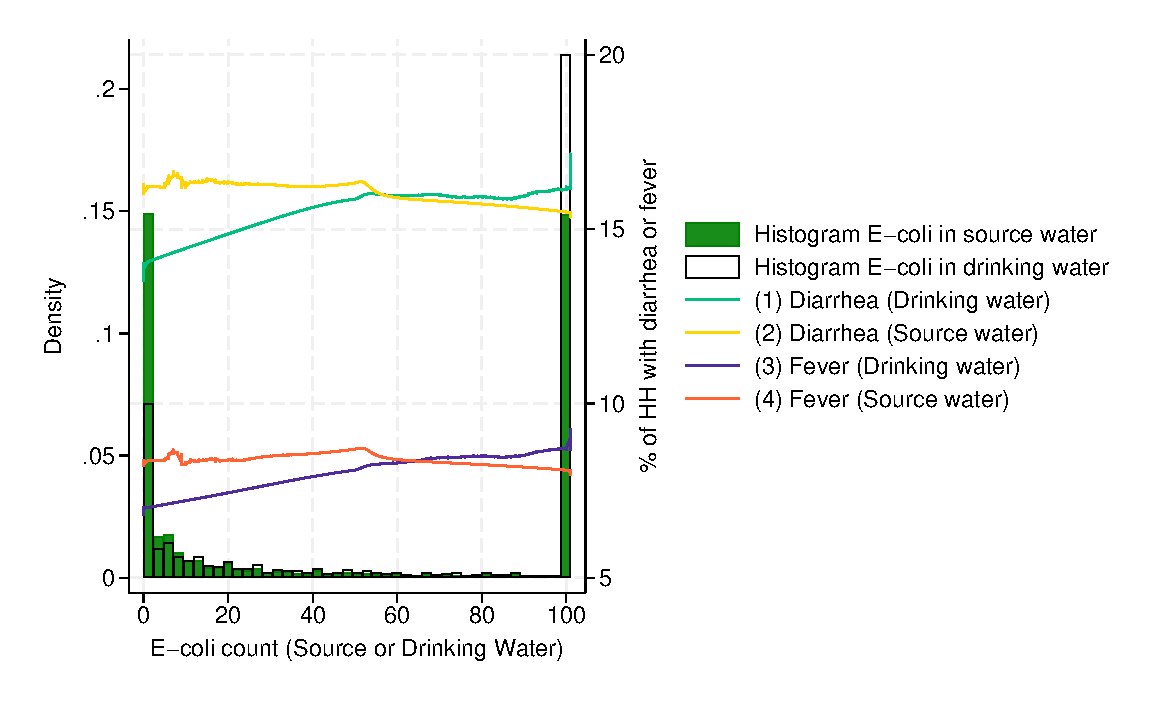
\includegraphics[width=\textwidth]{WaterQ_Morbidity.eps}\end{subfigure}
{\footnotesize  \begin{flushleft} Notes: N=22,589 children under age five. The figure shows the relationship between E. coli counts in source and drinking water and the incidence of diarrhea and fever among households. The histograms show the distribution of E. coli counts in both source and drinking water.\end{flushleft}}
\end{figure}

\subsection{Water treatment and diarrhea}  
Figure \ref{Desc_0} shows the prevalence of diarrhea among children under age 5, grouped by household water treatment methods. While some countries exhibit a lower prevalence of diarrhea among households that treat their water, the difference is minor. In some instances, the relationship is reversed, with a higher prevalence of diarrhea observed among households that treat their water. Such patterns are widely observed, and several studies using MICS data do not find a clear link between water treatment and diarrhea \citep{husein2023examination}. 

The unclear relationship can be attributed to endogeneity. Households with contaminated water, which is correlated with higher diarrhea prevalence, are more likely to treat their water, while those using uncontaminated water sources are less likely to do so. Another reason for the weak link is the low efficacy of the water treatment itself.

\begin{figure}[htbp]\centering
\caption{Diarrhea prevalence among U5 children by water treatment methods}\label{Desc_0}
\begin{subfigure}[b]{1\textwidth}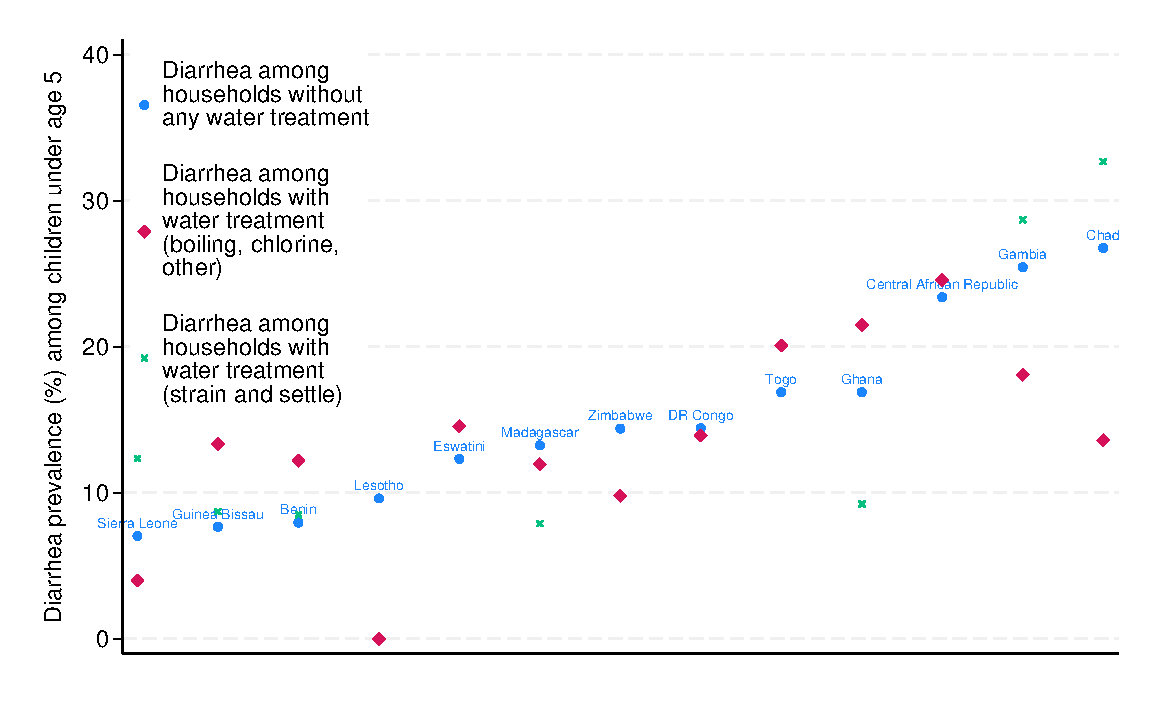
\includegraphics[width=\textwidth]{Water_Diarrhea_Treat.eps}\end{subfigure}
{\footnotesize  \begin{flushleft} Notes: The prevalence of diarrhea among children under age 5 across 14 countries from MICS, using nationally representative weights. Categories with fewer than 15 samples are excluded from the analysis, as the sample size is too small to calculate a reliable average.\end{flushleft}}
\end{figure}

\clearpage
\section{Causal Chain}
We identify the following causal chain:
\begin{equation}
M_{\text{source}} \to T \to M_{\text{drinking}} \to Y,
\end{equation}
where $M_{\text{source}}$ is the baseline water quality measured as CFU E. coli count, discretized as: 0 = No risk (0 CFU), 1 = Some risk ($1 \leq \text{CFU} < 100$), and 2 = Very high risk (CFU $\geq$ 100). This discretization is motivated by the fact that the original water quality variables are right-censored at 101 CFU.

$T$ denotes the treatment variable. We evaluate two treatment specifications: (1) \textit{Any treatment}: a binary indicator (0 = no treatment, 1 = any treatment), and (2) \textit{Multitreatment}: categorical treatment by type---boil, chlorine, filter, or other---each compared to the control (no treatment).

An important identification insight concerns the role of $M_{\text{source}}$. If we ignore the path $M_{\text{source}} \to T$, we end up comparing ``clean-source'' households who do not treat with ``dirty-source'' households who do treat. Because those who treat water are systematically starting from a worse baseline, a simple comparison would underestimate the effectiveness of treatment, as $M_{\text{source}}$ acts as a confounder. \footnote{Conversely, conditioning on $M_{\text{drinking}}$ in the base model would block the biological pathway (it acts as a mediator), which would lead to observing no treatment effect. Our empirical strategy therefore controls for $M_{\text{source}}$ but does not condition on $M_{\text{drinking}}$.}








\iffalse
\section{Notes}

%https://docs.doubleml.org/tutorial/stable/lectures/L1/introduction_part1.html#/neyman-orthogonality-motivation

Why Double Machine Learning?
$$Y=g_0(D,X) + U$$
ML Learner
, $$E(U|X,D)=0$$.
 

Why not simply estimate g0(D,X)
 with ML and plug in predictions $g_0(D,X)$?
ML methods address the variance-bias-tradeoff by introducing some kind of regularization
This will translate into a bias of the causal estimate


Challenges in causal machine learning
Causal estimation after using ML methods for estimation require adjustments of the estimation framework $\implies$ Chernozhukov et al. (2018)


The Key Ingredients of DML
1. Neyman orthogonality
2. High-quality ML estimation
3. Sample splitting






Motivation
We want to make estimation of the ATE robust against the regularization bias of ML learners

This can be achieved by using an orthogonal estimation framework

Neyman orthogonality states that the error terms that arise due to regularization do not affect the causal estimate.


Neyman orthogonality ensures that the moment condition identifying $\theta_0$ is insensitive to small perturbations of the nuisance function $\eta$ around $\eta_0$

Method uses doubly robust score.
Estiamtes propensity score:

\iffalse

The ℓ1
-penalization of Lasso would reduce some of the coefficients in γ=(γ1,γ2)
 towards zero and maybe set some of them exactly to zero, say γ2
 for the confounder X2

This is equivalent to removing the confounder X2
 from the causal model
⇒
 Ommited variable bias / confounding bias


 The nuisance parameters are estimated with high-quality (fast-enough converging) machine learning methods.

Different structural assumptions on η0
 lead to the use of different machine-learning tools for estimating η0
 (Chernozhukov et al. 2018, sec. 3)

Rate requirement in the IRM for estimation of ATE:
∥m^0−m0∥P,2×∥ℓ^0−ℓ0∥P,2≤δNN−1/2

⇒
 We can use ML methods, that have typically slower convergence rates than the parametric N1/2
 (as for a correctly specified linear regression model)




High-Quality ML Estimation: Use Case Example
Comparison of the performance of the ML-based causal model to estimation based on (unpenalized) logistic regression
print(dml_obj_linear.evaluate_learners())
print(dml_obj_linear.evaluate_learners(metric=balanced_accuracy))

{'ml_g0': array([[0.45735802]]), 'ml_g1': array([[0.44600344]]), 'ml_m': array([[0.48082561]])}
{'ml_g0': array([[0.49937559]]), 'ml_g1': array([[0.51025686]]), 'ml_m': array([[0.6107002]])}


print(dml_obj_orth.evaluate_learners())
print(dml_obj_orth.evaluate_learners(metric=balanced_accuracy))

{'ml_g0': array([[0.46770032]]), 'ml_g1': array([[0.44701511]]), 'ml_m': array([[0.4792336]])}
{'ml_g0': array([[0.51123643]]), 'ml_g1': array([[0.53925407]]), 'ml_m': array([[0.61656226]])}



Main Result: Double Machine Learning
Main result in Chernozhukov et al. (2018)
There exist regularity conditions, such that the DML estimator θ~0
 concentrates in a 1/N−−√
-neighborhood of θ0
 and the sampling error is approximately
N−−√(θ~0−θ0)∼N(0,σ2),
with
σ2:=J−20E(ψ2(W;θ0,η0)),J0=E(ψa(W;η0)).
\fi

\fi
\end{appendices}
\end{document}
}
